
% o conteúdo deste arquivo é gerado automaticamente pelo script
% bin/softwares-summary, favor não editar manualmente

\xchapter{Softwares acadêmicos}{Este capítulo ...}
\label{softwares-summary}

\begin{figure}[h]
  \center
  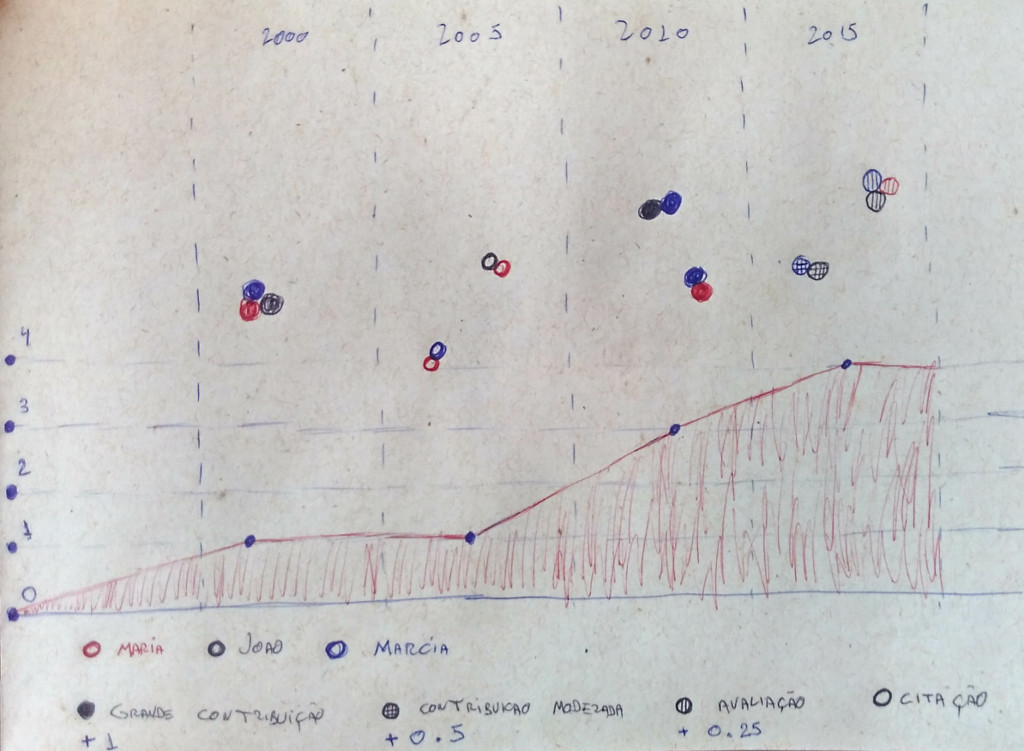
\includegraphics[scale=0.35]{imagens/software-timeline-wireframe.jpg}
  \caption{Protótipo do gráfico com timeline do software}
\end{figure}

\section{2LS - 2nd order Logic Solving}

Análise de terminação para programas C usando resumo interprocedural baseado em modelos
publicado no 2015, ASE,
disponibilizado em \url{http://svn.cprover.org/wiki/doku.php?id=2ls for program analysis}
como software livre
sob uma licença BSD.

Software com lançamentos ocasionais,
7 versões lançadas
entre 2015 e 2017,
escrito em C++,
uma busca por citações no {\bf IEEE Xplore} por
\texttt{(('2nd order Logic Solving') AND 2LS)}
e no {\bf ACM} por
\texttt{content.ftsec:(2LS) AND (order) AND (Logic) AND (Solving)}
retornou
37 resultados,
apenas um faz referência ao software.

\begin{itemize}
\item Chen Y. H. and David C. and Kroening D. and Schrammel P. and Wachter B.
      2015.
        \textbf{\textit{ Synthesising Interprocedural Bit-Precise Termination Proofs (T)}}.
      Peso:
      1 (
          cita
          usa
          contribui
          cria
      ),
      0 (
são os primeiros autores a publicar sobre o software
      ).
      Final:
      1

\end{itemize}

Peso total das referências por ano:

\begin{table}[h]
\caption{Número de citações ao 2LS  por ano}
\centering
\begin{tabular}{| l | c | c | c | c |}
  \hline
  Ano & Número de citações & Peso da contribuição & Peso da autoria & Peso final \\
  \hline
  2015
    & 1
    & 1.00
    & 0.00
    & 1.00 \\
  \hline
\end{tabular}
\end{table}


\section{AccessAnalysis}

Cálculo de métricas IGAT e IGAM
publicado no 2012, SCAM,
disponibilizado em \url{http://accessanalysis.sourceforge.net}
como software livre
sob uma licença EPL.

Software considerado obsoleto,
4 versões lançadas
entre 2010 e 2012,
escrito em Java,
uma busca por citações no {\bf IEEE Xplore} por
\texttt{(AccessAnalysis)}
e no {\bf ACM} por
\texttt{content.ftsec:(+AccessAnalysis +Tool +Java +Modifiers)}
retornou
8 resultados,
{\bf 2} fazem referência ao software.

\begin{itemize}
\item Zoller C. and Schmolitzky A.
      2012.
        \textit{ Measuring Inappropriate Generosity with Access Modifiers in Java Systems}.
      Peso:
      0.1 (
          cita
      ),
      0 (
são os primeiros autores a publicar sobre o software
      ).
      Final:
      0.1

\item Zoller C. and Schmolitzky A.
      2012.
        \textbf{\textit{ AccessAnalysis: A Tool for Measuring the Appropriateness of Access Modifiers in Java Systems}}.
      Peso:
      1 (
          cita
          usa
          contribui
          cria
      ),
      0 (
são os primeiros autores a publicar sobre o software
      ).
      Final:
      1

\end{itemize}

Peso total das referências por ano:

\begin{table}[h]
\caption{Número de citações ao AccessAnalysis por ano}
\centering
\begin{tabular}{| l | c | c | c | c |}
  \hline
  Ano & Número de citações & Peso da contribuição & Peso da autoria & Peso final \\
  \hline
  2012
    & 2
    & 1.10
    & 0.00
    & 1.10 \\
  \hline
\end{tabular}
\end{table}


\section{APIExample}

Extração de informações de API Java e documentação automática com exemplos
publicado no 2011, ASE,
disponibilizado em \url{http://www.apiexample.com}
mas inacessível em 09/08/2017.

Software sem informações sobre lançamentos ou releases,
uma busca por citações no {\bf IEEE Xplore} por
\texttt{((APIExample) AND Java)}
e no {\bf ACM} por
\texttt{content.ftsec:(+APIExample +Java)}
retornou
16 resultados,
{\bf 4} fazem referência ao software.

\begin{itemize}
\item Wang L. and Fang L. and Wang L. and Li G. and Xie B. and Yang F.
      2011.
        \textbf{\textit{ APIExample: An effective web search based usage example recommendation system for java APIs}}.
      Peso:
      1 (
          cita
          usa
          contribui
          cria
      ),
      0 (
são os primeiros autores a publicar sobre o software
      ).
      Final:
      1

\item Montandon E. J. and Borges H. and Felix D. and Valente T. M.
      2013.
        \textit{ Documenting APIs with examples: Lessons learned with the APIMiner platform}.
      Peso:
      0.1 (
          cita
      ),
      0.5 (
nenhum dos autores publicou sobre o software antes
      ).
      Final:
      0.15

\item Zhu Z. and Zou Y. and Jin Y. and Xie B.
      2013.
        \textit{ Generating API-usage Example for Project Developers}.
      Peso:
      0.1 (
          cita
      ),
      0.25 (
uma parte dos autores já publicou sobre o software em anos anteriores
      ).
      Final:
      0.125

\item Yu H. and Song W. and Mine T.
      2016.
        \textit{ APIBook: An Effective Approach for Finding APIs}.
      Peso:
      0.1 (
          cita
      ),
      0.5 (
nenhum dos autores publicou sobre o software antes
      ).
      Final:
      0.15

\end{itemize}

Peso total das referências por ano:

\begin{table}[h]
\caption{Número de citações ao APIExample por ano}
\centering
\begin{tabular}{| l | c | c | c | c |}
  \hline
  Ano & Número de citações & Peso da contribuição & Peso da autoria & Peso final \\
  \hline
  2011
    & 1
    & 1.00
    & 0.00
    & 1.00 \\
  2013
    & 2
    & 0.20
    & 0.75
    & 0.28 \\
  2016
    & 1
    & 0.10
    & 0.50
    & 0.15 \\
  \hline
\end{tabular}
\end{table}


\section{BEG - Bandera environment generator}

Criação automática de ambientes para verificação de modelos Java
publicado no 2003, ASE,
disponibilizado em \url{http://bandera.projects.cs.ksu.edu/}
mas inacessível em 09/08/2017.

Software sem informações sobre lançamentos ou releases,
uma busca por citações no {\bf IEEE Xplore} por
\texttt{(("Bandera environment generator") AND BEG)}
e no {\bf ACM} por
\texttt{content.ftsec:(+"Bandera environment generator" +BEG)}
retornou
10 resultados,
{\bf 9} fazem referência ao software.

\begin{itemize}
\item Tkachuk O. and Dwyer B. M. and Pasareanu S. C.
      2003.
        \textbf{\textit{ Automated environment generation for software model checking}}.
      Peso:
      1 (
          cita
          usa
          contribui
          cria
      ),
      0 (
são os primeiros autores a publicar sobre o software
      ).
      Final:
      1

\item Dwyer B. M. and Robby and Tkachuk O. and Visser W.
      2004.
        \textit{ Analyzing interaction orderings with model checking}.
      Peso:
      0.25 (
          cita
          usa
      ),
      0.25 (
uma parte dos autores já publicou sobre o software em anos anteriores
      ).
      Final:
      0.3125

\item Tkachuk O. and Rajan P. S.
      2006.
        \textit{ Application of Automated Environment Generation to Commercial Software}.
      Peso:
      0.25 (
          cita
          usa
      ),
      0.25 (
uma parte dos autores já publicou sobre o software em anos anteriores
      ).
      Final:
      0.3125

\item Mutilin V.
      2006.
        \textit{ Concurrent Testing of Java Components Using Java PathFinder}.
      Peso:
      0.1 (
          cita
      ),
      0.25 (
uma parte dos autores já publicou sobre o software em anos anteriores
      ).
      Final:
      0.125

\item Tkachuk O. and Rajan P. S.
      2007.
        \textit{ Combining Environment Generation and Slicing for Modular Software Model Checking}.
      Peso:
      0.25 (
          cita
          usa
      ),
      0.25 (
uma parte dos autores já publicou sobre o software em anos anteriores
      ).
      Final:
      0.3125

\item Parizek P. and Plasil F.
      2007.
        \textit{ Partial Verification of Software Components: Heuristics for Environment Construction}.
      Peso:
      0.1 (
          cita
      ),
      0.5 (
nenhum dos autores publicou sobre o software antes
      ).
      Final:
      0.15

\item Tkachuk O. and Dwyer B. M.
      2010.
        \textit{ Environment generation for validating event-driven software using model checking}.
      Peso:
      0.5 (
          cita
          usa
          contribui
      ),
      0.1 (
todos os autores já publicaram sobre o software em anos anteriores
      ).
      Final:
      0.55

\item Parizek P. and Plasil F.
      2010.
        \textit{ Assume-guarantee verification of software components in SOFA 2 framework}.
      Peso:
      0.1 (
          cita
      ),
      0.1 (
todos os autores já publicaram sobre o software em anos anteriores
      ).
      Final:
      0.11

\item Siavashi F. and Truscan D.
      2015.
        \textit{ Environment Modeling in Model-based Testing: Concepts, Prospects and Research Challenges: A Systematic Literature Review}.
      Peso:
      0.1 (
          cita
      ),
      0.5 (
nenhum dos autores publicou sobre o software antes
      ).
      Final:
      0.15

\end{itemize}

Peso total das referências por ano:

\begin{table}[h]
\caption{Número de citações ao BEG  por ano}
\centering
\begin{tabular}{| l | c | c | c | c |}
  \hline
  Ano & Número de citações & Peso da contribuição & Peso da autoria & Peso final \\
  \hline
  2003
    & 1
    & 1.00
    & 0.00
    & 1.00 \\
  2004
    & 1
    & 0.25
    & 0.25
    & 0.31 \\
  2006
    & 2
    & 0.35
    & 0.50
    & 0.44 \\
  2007
    & 2
    & 0.35
    & 0.75
    & 0.46 \\
  2010
    & 2
    & 0.60
    & 0.20
    & 0.66 \\
  2015
    & 1
    & 0.10
    & 0.50
    & 0.15 \\
  \hline
\end{tabular}
\end{table}


\section{ccJava - Class-based Crosscutting Language for Java}

Linguagem orientada a aspectos
publicado no 2007, ASE,
disponibilizado em \url{http://posl.minnie.ai.kyutech.ac.jp/}
mas inacessível em 09/08/2017.

Software sem informações sobre lançamentos ou releases,
uma busca por citações no {\bf IEEE Xplore} por
\texttt{(ccJava)}
e no {\bf ACM} por
\texttt{content.ftsec:(+ccJava)}
retornou
7 resultados,
{\bf 5} fazem referência ao software.

\begin{itemize}
\item Ubayashi N. and Sakai A. and Tamai T.
      2007.
        \textbf{\textit{ An Aspect-oriented Weaving Mechanism Based on Component and Connector Architecture}}.
      Peso:
      1 (
          cita
          usa
          contribui
          cria
      ),
      0 (
são os primeiros autores a publicar sobre o software
      ).
      Final:
      1

\item Ubayashi N. and Sakai A. and Tamai T.
      2007.
        \textit{ An Interface Mechanism for Encapsulating Weaving in Class-based AOP}.
      Peso:
      0.1 (
          cita
      ),
      0 (
são os primeiros autores a publicar sobre o software
      ).
      Final:
      0.1

\item Ubayashi N. and Sato Y. and Sakai A. and Tamai T.
      2008.
        \textit{ Alloy-Based Lightweight Verification for Aspect-Oriented Architecture}.
      Peso:
      0.5 (
          cita
          usa
          contribui
      ),
      0 (
são os primeiros autores a publicar sobre o software
      ).
      Final:
      0.5

\item Ubayashi N. and Akatoki H. and Nomura J.
      2009.
        \textit{ Pointcut-based Architectural Interface for Bridging a Gap Between Design and Implementation}.
      Peso:
      0.5 (
          cita
          usa
          contribui
      ),
      0.25 (
uma parte dos autores já publicou sobre o software em anos anteriores
      ).
      Final:
      0.625

\item Ubayashi N. and Nomura J. and Tamai T.
      2010.
        \textit{ Archface: a contract place where architectural design and code meet together}.
      Peso:
      0.1 (
          cita
      ),
      0.1 (
todos os autores já publicaram sobre o software em anos anteriores
      ).
      Final:
      0.11

\end{itemize}

Peso total das referências por ano:

\begin{table}[h]
\caption{Número de citações ao ccJava  por ano}
\centering
\begin{tabular}{| l | c | c | c | c |}
  \hline
  Ano & Número de citações & Peso da contribuição & Peso da autoria & Peso final \\
  \hline
  2007
    & 2
    & 1.10
    & 0.00
    & 1.10 \\
  2008
    & 1
    & 0.50
    & 0.00
    & 0.50 \\
  2009
    & 1
    & 0.50
    & 0.25
    & 0.62 \\
  2010
    & 1
    & 0.10
    & 0.10
    & 0.11 \\
  \hline
\end{tabular}
\end{table}


\section{CIVL - Concurrency intermediate verification language}

Framework para verificação de programas concorrentes
publicado no 2015, ASE,
disponibilizado em \url{http://vsl.cis.udel.edu/civl/}
como software livre
sob uma licença GPL.

Software com lançamentos frequentes,
36 versões lançadas
entre 2015 e 2017,
escrito em C,
uma busca por citações no {\bf IEEE Xplore} por
\texttt{(('concurrency intermediate verification') AND CIVL)}
e no {\bf ACM} por
\texttt{content.ftsec:(+civl +concurrency +intermediate +verification +language)}
retornou
8 resultados,
{\bf 6} fazem referência ao software.

\begin{itemize}
\item Gopalakrishnan G. and Sawaya J.
      2015.
        \textit{ Achieving Formal Parallel Program Debugging by Incentivizing CS/HPC Collaborative Tool Development}.
      Peso:
      0.1 (
          cita
      ),
      0 (
são os primeiros autores a publicar sobre o software
      ).
      Final:
      0.1

\item L\'{o}pez A. H. and Marques B. R. E. and Martins F. and Ng N. and Santos C. and Vasconcelos T. V. and Yoshida N.
      2015.
        \textit{ Protocol-based Verification of Message-passing Parallel Programs}.
      Peso:
      0.1 (
          cita
      ),
      0 (
são os primeiros autores a publicar sobre o software
      ).
      Final:
      0.1

\item Zheng M. and Rogers S. M. and Luo Z. and Dwyer B. M. and Siegel F. S.
      2015.
        \textbf{\textit{ CIVL: Formal Verification of Parallel Programs}}.
      Peso:
      1 (
          cita
          usa
          contribui
          cria
      ),
      0 (
são os primeiros autores a publicar sobre o software
      ).
      Final:
      1

\item Siegel F. S. and Zheng M. and Luo Z. and Zirkel K. T. and Marianiello V. A. and Edenhofner G. J. and Dwyer B. M. and Rogers S. M.
      2015.
        \textit{ CIVL: The Concurrency Intermediate Verification Language}.
      Peso:
      0.1 (
          cita
      ),
      0 (
são os primeiros autores a publicar sobre o software
      ).
      Final:
      0.1

\item Siegel F. S.
      2017.
        \textit{ CIVL Solutions to Verifythis 2016 Challenges}.
      Peso:
      0.1 (
          cita
      ),
      0.1 (
todos os autores já publicaram sobre o software em anos anteriores
      ).
      Final:
      0.11

\item Jasper M. and Fecke M. and Steffen B. and Schordan M. and Meijer J. and Pol de van J. and Howar F. and Siegel F. S.
      2017.
        \textit{ The RERS 2017 Challenge and Workshop (Invited Paper)}.
      Peso:
      0.1 (
          cita
      ),
      0.25 (
uma parte dos autores já publicou sobre o software em anos anteriores
      ).
      Final:
      0.125

\end{itemize}

Peso total das referências por ano:

\begin{table}[h]
\caption{Número de citações ao CIVL  por ano}
\centering
\begin{tabular}{| l | c | c | c | c |}
  \hline
  Ano & Número de citações & Peso da contribuição & Peso da autoria & Peso final \\
  \hline
  2015
    & 4
    & 1.30
    & 0.00
    & 1.30 \\
  2017
    & 2
    & 0.20
    & 0.35
    & 0.24 \\
  \hline
\end{tabular}
\end{table}


\section{CodeBoost}

Transformação source-to-source para otimização de programas C++
publicado no 2003, SCAM,
disponibilizado em \url{http://codeboost.org}
como software livre
sob uma licença GPL v2.

Software com lançamentos ocasionais,
134 versões lançadas
entre 2000 e 2004,
escrito em C,
uma busca por citações no {\bf IEEE Xplore} por
\texttt{((CodeBoost) AND C++)}
e no {\bf ACM} por
\texttt{content.ftsec:(+CodeBoost +"C++" +Tool)}
retornou
25 resultados,
{\bf 15} fazem referência ao software.

\begin{itemize}
\item L\"{a}mmel R. and Visser E. and Visser J.
      2003.
        \textit{ Strategic Programming Meets Adaptive Programming}.
      Peso:
      0.1 (
          cita
      ),
      0 (
são os primeiros autores a publicar sobre o software
      ).
      Final:
      0.1

\item Bagge S. O. and Kalleberg T. K. and Haveraaen M. and Visser E.
      2003.
        \textbf{\textit{ Design of the CodeBoost transformation system for domain-specific optimisation of C++ programs}}.
      Peso:
      1 (
          cita
          usa
          contribui
          cria
      ),
      0 (
são os primeiros autores a publicar sobre o software
      ).
      Final:
      1

\item Visser E.
      2005.
        \textit{ Transformations for abstractions}.
      Peso:
      0.1 (
          cita
      ),
      0.1 (
todos os autores já publicaram sobre o software em anos anteriores
      ).
      Final:
      0.11

\item Schordan M. and Quinlan D.
      2005.
        \textit{ Specifying transformation sequences as computation on program fragments with an abstract attribute grammar}.
      Peso:
      0.1 (
          cita
      ),
      0.25 (
uma parte dos autores já publicou sobre o software em anos anteriores
      ).
      Final:
      0.125

\item Mernik M. and Heering J. and Sloane M. A.
      2005.
        \textit{ When and How to Develop Domain-specific Languages}.
      Peso:
      0.1 (
          cita
      ),
      0.25 (
uma parte dos autores já publicou sobre o software em anos anteriores
      ).
      Final:
      0.125

\item Quinlan D. and Schordan M. and Vuduc R. and Yi Q.
      2006.
        \textit{ Annotating user-defined abstractions for optimization}.
      Peso:
      0.1 (
          cita
      ),
      0.25 (
uma parte dos autores já publicou sobre o software em anos anteriores
      ).
      Final:
      0.125

\item Bravenboer M. and Kalleberg T. K. and Vermaas R. and Visser E.
      2006.
        \textit{ Stratego/XT 0.16: Components for Transformation Systems}.
      Peso:
      0.1 (
          cita
      ),
      0.25 (
uma parte dos autores já publicou sobre o software em anos anteriores
      ).
      Final:
      0.125

\item Gottschling P. and Lumsdaine A.
      2008.
        \textit{ Integrating Semantics and Compilation: Using C++ Concepts to Develop Robust and Efficient Reusable Libraries}.
      Peso:
      0.1 (
          cita
      ),
      0.5 (
nenhum dos autores publicou sobre o software antes
      ).
      Final:
      0.15

\item Willcock J. J. and Lumsdaine A. and Quinlan J. D.
      2009.
        \textit{ Reusable, Generic Program Analyses and Transformations}.
      Peso:
      0.1 (
          cita
      ),
      0.25 (
uma parte dos autores já publicou sobre o software em anos anteriores
      ).
      Final:
      0.125

\item Tang X. and J\"{a}rvi J.
      2010.
        \textit{ Generic Flow-sensitive Optimizing Transformations in C++ with Concepts}.
      Peso:
      0.1 (
          cita
      ),
      0.5 (
nenhum dos autores publicou sobre o software antes
      ).
      Final:
      0.15

\item Chafi H. and Sujeeth K. A. and Brown J. K. and Lee H. and Atreya R. A. and Olukotun K.
      2011.
        \textit{ A Domain-specific Approach to Heterogeneous Parallelism}.
      Peso:
      0.1 (
          cita
      ),
      0.5 (
nenhum dos autores publicou sobre o software antes
      ).
      Final:
      0.15

\item Brown J. K. and Sujeeth K. A. and Lee J. H. and Rompf T. and Chafi H. and Odersky M. and Olukotun K.
      2011.
        \textit{ A Heterogeneous Parallel Framework for Domain-Specific Languages}.
      Peso:
      0.1 (
          cita
      ),
      0.5 (
nenhum dos autores publicou sobre o software antes
      ).
      Final:
      0.15

\item Hong S. and Chafi H. and Sedlar E. and Olukotun K.
      2012.
        \textit{ Green-Marl: A DSL for Easy and Efficient Graph Analysis}.
      Peso:
      0.1 (
          cita
      ),
      0.25 (
uma parte dos autores já publicou sobre o software em anos anteriores
      ).
      Final:
      0.125

\item Keep W. A. and Dybvig K. R.
      2013.
        \textit{ A Nanopass Framework for Commercial Compiler Development}.
      Peso:
      0.1 (
          cita
      ),
      0.5 (
nenhum dos autores publicou sobre o software antes
      ).
      Final:
      0.15

\item Scherr M. and Chiba S.
      2015.
        \textit{ Almost First-class Language Embedding: Taming Staged Embedded DSLs}.
      Peso:
      0.1 (
          cita
      ),
      0.5 (
nenhum dos autores publicou sobre o software antes
      ).
      Final:
      0.15

\end{itemize}

Peso total das referências por ano:

\begin{table}[h]
\caption{Número de citações ao CodeBoost por ano}
\centering
\begin{tabular}{| l | c | c | c | c |}
  \hline
  Ano & Número de citações & Peso da contribuição & Peso da autoria & Peso final \\
  \hline
  2003
    & 2
    & 1.10
    & 0.00
    & 1.10 \\
  2005
    & 3
    & 0.30
    & 0.60
    & 0.36 \\
  2006
    & 2
    & 0.20
    & 0.50
    & 0.25 \\
  2008
    & 1
    & 0.10
    & 0.50
    & 0.15 \\
  2009
    & 1
    & 0.10
    & 0.25
    & 0.12 \\
  2010
    & 1
    & 0.10
    & 0.50
    & 0.15 \\
  2011
    & 2
    & 0.20
    & 1.00
    & 0.30 \\
  2012
    & 1
    & 0.10
    & 0.25
    & 0.12 \\
  2013
    & 1
    & 0.10
    & 0.50
    & 0.15 \\
  2015
    & 1
    & 0.10
    & 0.50
    & 0.15 \\
  \hline
\end{tabular}
\end{table}


\section{CSL - Composite Symbolic Library}

Verificação de modelos
publicado no 2001, ASE,
disponibilizado em \url{http://www.cs.ucsb.edu/~bultan/composite/}
gratuitamente
sem uma licença definida.

Software sem informações sobre lançamentos ou releases,
escrito em C,
uma busca por citações no {\bf IEEE Xplore} por
\texttt{((((composite) AND bultan) AND Action Language Verifier) OR ("Composite Symbolic Library"))}
e no {\bf ACM} por
\texttt{content.ftsec:(+composite +"Action Language Verifier")}
retornou
14 resultados,
{\bf 6} fazem referência ao software.

\begin{itemize}
\item Bultan T. and Yavuz-Kahveci T.
      2001.
        \textbf{\textit{ Action Language Verifier}}.
      Peso:
      1 (
          cita
          usa
          contribui
          cria
      ),
      0 (
são os primeiros autores a publicar sobre o software
      ).
      Final:
      1

\item Fu X. and Bultan T. and Su J.
      2004.
        \textit{ Realizability of conversation protocols with message contents}.
      Peso:
      0.1 (
          cita
      ),
      0.25 (
uma parte dos autores já publicou sobre o software em anos anteriores
      ).
      Final:
      0.125

\item Zhang D. and Cleaveland R.
      2005.
        \textit{ Efficient Temporal-logic Query Checking for Presburger Systems}.
      Peso:
      0.1 (
          cita
      ),
      0.5 (
nenhum dos autores publicou sobre o software antes
      ).
      Final:
      0.15

\item Bultan T. and Heitmeyer C.
      2006.
        \textit{ Analyzing tabular requirements specifications using infinite state model checking}.
      Peso:
      0.1 (
          cita
      ),
      0.25 (
uma parte dos autores já publicou sobre o software em anos anteriores
      ).
      Final:
      0.125

\item Yang Z. and Wang C. and Gupta A. and Ivancic F.
      2006.
        \textit{ Mixed Symbolic Representations for Model Checking Software Programs}.
      Peso:
      0.5 (
          cita
          usa
          contribui
      ),
      0.25 (
uma parte dos autores já publicou sobre o software em anos anteriores
      ).
      Final:
      0.625

\item Yang Z. and Wang C. and Gupta A. and Ivan\v{c}i\'{c} F.
      2009.
        \textit{ Model Checking Sequential Software Programs via Mixed Symbolic Analysis}.
      Peso:
      0.25 (
          cita
          usa
      ),
      0.25 (
uma parte dos autores já publicou sobre o software em anos anteriores
      ).
      Final:
      0.3125

\end{itemize}

Peso total das referências por ano:

\begin{table}[h]
\caption{Número de citações ao CSL  por ano}
\centering
\begin{tabular}{| l | c | c | c | c |}
  \hline
  Ano & Número de citações & Peso da contribuição & Peso da autoria & Peso final \\
  \hline
  2001
    & 1
    & 1.00
    & 0.00
    & 1.00 \\
  2004
    & 1
    & 0.10
    & 0.25
    & 0.12 \\
  2005
    & 1
    & 0.10
    & 0.50
    & 0.15 \\
  2006
    & 2
    & 0.60
    & 0.50
    & 0.75 \\
  2009
    & 1
    & 0.25
    & 0.25
    & 0.31 \\
  \hline
\end{tabular}
\end{table}


\section{CPA+ - Configurable program analysis with dynamic precision adjustment}

Análise configurável de programa com ajuste dinâmico de precisão
publicado no 2008, ASE,
disponibilizado em \url{http://www.cs.sfu.ca/~dbeyer/blast_cpaplus/}
mas inacessível em 09/08/2017.

Software sem informações sobre lançamentos ou releases,
uma busca por citações no {\bf IEEE Xplore} por
\texttt{(('program analysis') AND cpa+)}
e no {\bf ACM} por
\texttt{content.ftsec:(+cpa +dbeyer)}
retornou
8 resultados,
{\bf 5} fazem referência ao software.

\begin{itemize}
\item Beyer D. and Henzinger A. T. and Theoduloz G.
      2008.
        \textbf{\textit{ Program Analysis with Dynamic Precision Adjustment}}.
      Peso:
      1 (
          cita
          usa
          contribui
          cria
      ),
      0 (
são os primeiros autores a publicar sobre o software
      ).
      Final:
      1

\item Beyer D. and Keremoglu E. M. and Wendler P.
      2010.
        \textit{ Predicate Abstraction with Adjustable-block Encoding}.
      Peso:
      0.5 (
          cita
          usa
          contribui
      ),
      0.25 (
uma parte dos autores já publicou sobre o software em anos anteriores
      ).
      Final:
      0.625

\item Beyer D. and Henzinger A. T. and Keremoglu E. M. and Wendler P.
      2012.
        \textit{ Conditional Model Checking: A Technique to Pass Information Between Verifiers}.
      Peso:
      0.5 (
          cita
          usa
          contribui
      ),
      0.1 (
todos os autores já publicaram sobre o software em anos anteriores
      ).
      Final:
      0.55

\item Beyer D. and L\"{o}we S. and Novikov E. and Stahlbauer A. and Wendler P.
      2013.
        \textit{ Precision Reuse for Efficient Regression Verification}.
      Peso:
      0.5 (
          cita
          usa
          contribui
      ),
      0.25 (
uma parte dos autores já publicou sobre o software em anos anteriores
      ).
      Final:
      0.625

\item Beyer D. and Dangl M. and Dietsch D. and Heizmann M. and Stahlbauer A.
      2015.
        \textit{ Witness Validation and Stepwise Testification Across Software Verifiers}.
      Peso:
      0.5 (
          cita
          usa
          contribui
      ),
      0.25 (
uma parte dos autores já publicou sobre o software em anos anteriores
      ).
      Final:
      0.625

\end{itemize}

Peso total das referências por ano:

\begin{table}[h]
\caption{Número de citações ao CPA+  por ano}
\centering
\begin{tabular}{| l | c | c | c | c |}
  \hline
  Ano & Número de citações & Peso da contribuição & Peso da autoria & Peso final \\
  \hline
  2008
    & 1
    & 1.00
    & 0.00
    & 1.00 \\
  2010
    & 1
    & 0.50
    & 0.25
    & 0.62 \\
  2012
    & 1
    & 0.50
    & 0.10
    & 0.55 \\
  2013
    & 1
    & 0.50
    & 0.25
    & 0.62 \\
  2015
    & 1
    & 0.50
    & 0.25
    & 0.62 \\
  \hline
\end{tabular}
\end{table}


\section{CSeq}

Transformação source-to-source para programas C concorrentes
publicado no 2013, ASE,
disponibilizado em \url{http://users.ecs.soton.ac.uk/gp4/cseq/files/cseq-0.5.zip}
como software livre
sob uma licença BSD.

Software sem informações sobre lançamentos ou releases,
escrito em C,
uma busca por citações no {\bf IEEE Xplore} por
\texttt{((CSeq) AND soton)}
e no {\bf ACM} por
\texttt{content.ftsec:(+cseq +sequential +verification +tool)}
retornou
16 resultados,
{\bf 5} fazem referência ao software.

\begin{itemize}
\item Fischer B. and Inverso O. and Parlato G.
      2013.
        \textbf{\textit{ CSeq: A concurrency pre-processor for sequential C verification tools}}.
      Peso:
      1 (
          cita
          usa
          contribui
          cria
      ),
      0 (
são os primeiros autores a publicar sobre o software
      ).
      Final:
      1

\item Inverso O. and Nguyen L. T. and Fischer B. and Torre L. S. and Parlato G.
      2015.
        \textit{ Lazy-CSeq: A Context-Bounded Model Checking Tool for Multi-threaded C-Programs}.
      Peso:
      0.5 (
          cita
          usa
          contribui
      ),
      0 (
são os primeiros autores a publicar sobre o software
      ).
      Final:
      0.5

\item Bouajjani A. and Emmi M. and Enea C. and Hamza J.
      2015.
        \textit{ Tractable Refinement Checking for Concurrent Objects}.
      Peso:
      0.25 (
          cita
          usa
      ),
      0 (
são os primeiros autores a publicar sobre o software
      ).
      Final:
      0.25

\item Tomasco E. and Nguyen L. T. and Inverso O. and Fischer B. and L. Torre S. and Parlato G.
      2016.
        \textit{ Lazy Sequentialization for TSO and PSO via Shared Memory Abstractions}.
      Peso:
      0.25 (
          cita
          usa
      ),
      0.25 (
uma parte dos autores já publicou sobre o software em anos anteriores
      ).
      Final:
      0.3125

\item Mayer M. and Madhavan R.
      2016.
        \textit{ A Scala Library for Testing Student Assignments on Concurrent Programming}.
      Peso:
      0.1 (
          cita
      ),
      0.25 (
uma parte dos autores já publicou sobre o software em anos anteriores
      ).
      Final:
      0.125

\end{itemize}

Peso total das referências por ano:

\begin{table}[h]
\caption{Número de citações ao CSeq por ano}
\centering
\begin{tabular}{| l | c | c | c | c |}
  \hline
  Ano & Número de citações & Peso da contribuição & Peso da autoria & Peso final \\
  \hline
  2013
    & 1
    & 1.00
    & 0.00
    & 1.00 \\
  2015
    & 2
    & 0.75
    & 0.00
    & 0.75 \\
  2016
    & 2
    & 0.35
    & 0.50
    & 0.44 \\
  \hline
\end{tabular}
\end{table}


\section{DDVerify}

Verificação de Linux drivers através de checagem de modelos
publicado no 2007, ASE,
disponibilizado em \url{http://www.verify.ethz.ch/ddverify}
mas inacessível em 09/08/2017.

Software sem informações sobre lançamentos ou releases,
uma busca por citações no {\bf IEEE Xplore} por
\texttt{(DDVerify)}
e no {\bf ACM} por
\texttt{content.ftsec:(+DDVerify)}
retornou
4 resultados,
{\bf 3} fazem referência ao software.

\begin{itemize}
\item Witkowski T. and Blanc N. and Kroening D. and Weissenbacher G.
      2007.
        \textbf{\textit{ Model Checking Concurrent Linux Device Drivers}}.
      Peso:
      1 (
          cita
          usa
          contribui
          cria
      ),
      0 (
são os primeiros autores a publicar sobre o software
      ).
      Final:
      1

\item Blanc N. and Kroening D.
      2008.
        \textit{ Race analysis for SystemC using model checking}.
      Peso:
      0.1 (
          cita
      ),
      0.1 (
todos os autores já publicaram sobre o software em anos anteriores
      ).
      Final:
      0.11

\item Dileep P. K. and Raghavendra A. and Suman M. and Devesh G. and Srikanth V. S.
      2014.
        \textit{ Rules based automatic Linux Device Driver Verifier And Code Assistance}.
      Peso:
      0.1 (
          cita
      ),
      0.5 (
nenhum dos autores publicou sobre o software antes
      ).
      Final:
      0.15

\end{itemize}

Peso total das referências por ano:

\begin{table}[h]
\caption{Número de citações ao DDVerify por ano}
\centering
\begin{tabular}{| l | c | c | c | c |}
  \hline
  Ano & Número de citações & Peso da contribuição & Peso da autoria & Peso final \\
  \hline
  2007
    & 1
    & 1.00
    & 0.00
    & 1.00 \\
  2008
    & 1
    & 0.10
    & 0.10
    & 0.11 \\
  2014
    & 1
    & 0.10
    & 0.50
    & 0.15 \\
  \hline
\end{tabular}
\end{table}


\section{Derailer}

Localização de falhas de segurança em aplicações web
publicado no 2014, ASE,
disponibilizado em \url{http://people.csail.mit.edu/jnear/derailer}
como software livre
sob uma licença GPL v3.

Software considerado obsoleto,
2 versões lançadas
entre 2013 e 2014,
escrito em Ruby,
uma busca por citações no {\bf IEEE Xplore} por
\texttt{((Derailer) AND jnear)}
e no {\bf ACM} por
\texttt{content.ftsec:(+Derailer +analysis +security +web +tool +bugs +ruby)}
retornou
7 resultados,
{\bf 2} fazem referência ao software.

\begin{itemize}
\item Near P. J. and Jackson D.
      2014.
        \textbf{\textit{ Derailer: Interactive Security Analysis for Web Applications}}.
      Peso:
      1 (
          cita
          usa
          contribui
          cria
      ),
      0 (
são os primeiros autores a publicar sobre o software
      ).
      Final:
      1

\item Near P. J. and Jackson D.
      2016.
        \textit{ Finding Security Bugs in Web Applications Using a Catalog of Access Control Patterns}.
      Peso:
      0.1 (
          cita
      ),
      0.1 (
todos os autores já publicaram sobre o software em anos anteriores
      ).
      Final:
      0.11

\end{itemize}

Peso total das referências por ano:

\begin{table}[h]
\caption{Número de citações ao Derailer por ano}
\centering
\begin{tabular}{| l | c | c | c | c |}
  \hline
  Ano & Número de citações & Peso da contribuição & Peso da autoria & Peso final \\
  \hline
  2014
    & 1
    & 1.00
    & 0.00
    & 1.00 \\
  2016
    & 1
    & 0.10
    & 0.10
    & 0.11 \\
  \hline
\end{tabular}
\end{table}


\section{Diagnosys}

Construção de interfaces de debug para o kernel Linux
publicado no 2012, ASE,
disponibilizado em \url{http://momentum.labri.fr/projects/diagnosys}
mas inacessível em 09/08/2017.

Software sem informações sobre lançamentos ou releases,
uma busca por citações no {\bf IEEE Xplore} por
\texttt{((Diagnosys) AND debugging)}
e no {\bf ACM} por
\texttt{content.ftsec:(+"Diagnosys tool" +Debugging +Linux +"device drivers")}
retornou
9 resultados,
apenas um faz referência ao software.

\begin{itemize}
\item Bissyandé F. T. and Réveillère L. and Lawall L. J. and Muller G.
      2012.
        \textbf{\textit{ Diagnosys: automatic generation of a debugging interface to the Linux kernel}}.
      Peso:
      1 (
          cita
          usa
          contribui
          cria
      ),
      0 (
são os primeiros autores a publicar sobre o software
      ).
      Final:
      1

\end{itemize}

Peso total das referências por ano:

\begin{table}[h]
\caption{Número de citações ao Diagnosys por ano}
\centering
\begin{tabular}{| l | c | c | c | c |}
  \hline
  Ano & Número de citações & Peso da contribuição & Peso da autoria & Peso final \\
  \hline
  2012
    & 1
    & 1.00
    & 0.00
    & 1.00 \\
  \hline
\end{tabular}
\end{table}


\section{DOMPLETION}

Sugestão de código javascript
publicado no 2014, ASE,
disponibilizado em \url{https://github.com/saltlab/dompletion}
gratuitamente
sem uma licença definida.

Software sem informações sobre lançamentos ou releases,
escrito em Javascript,
uma busca por citações no {\bf IEEE Xplore} por
\texttt{content.ftsec:(+dompletion +JavaScript)}
e no {\bf ACM} por
\texttt{((dompletion) AND JavaScript)}
retornou
2 resultados,
{\bf 2} fazem referência ao software.

\begin{itemize}
\item Bajaj K. and Pattabiraman K. and Mesbah A.
      2014.
        \textbf{\textit{ Dompletion: DOM-aware JavaScript Code Completion}}.
      Peso:
      1 (
          cita
          usa
          contribui
          cria
      ),
      0 (
são os primeiros autores a publicar sobre o software
      ).
      Final:
      1

\item Bajaj K. and Pattabiraman K. and Mesbah A.
      2015.
        \textit{ LED: Tool for Synthesizing Web Element Locators}.
      Peso:
      0.1 (
          cita
      ),
      0.1 (
todos os autores já publicaram sobre o software em anos anteriores
      ).
      Final:
      0.11

\end{itemize}

Peso total das referências por ano:

\begin{table}[h]
\caption{Número de citações ao DOMPLETION por ano}
\centering
\begin{tabular}{| l | c | c | c | c |}
  \hline
  Ano & Número de citações & Peso da contribuição & Peso da autoria & Peso final \\
  \hline
  2014
    & 1
    & 1.00
    & 0.00
    & 1.00 \\
  2015
    & 1
    & 0.10
    & 0.10
    & 0.11 \\
  \hline
\end{tabular}
\end{table}


\section{DRC - Dangling Reference Checker}

Análise estática para detecção de referências inválidas em código dinâmico PHP
publicado no 2013, ASE,
disponibilizado em \url{http://home.engineering.iastate.edu/~hungnv/Research/DRC}
mas inacessível em 09/08/2017.

Software sem informações sobre lançamentos ou releases,
uma busca por citações no {\bf IEEE Xplore} por
\texttt{(DRC Dangling Reference Checker)}
e no {\bf ACM} por
\texttt{content.ftsec:(+DRC +Dangling +Reference)}
retornou
19 resultados,
{\bf 5} fazem referência ao software.

\begin{itemize}
\item Nguyen V. H. and Nguyen A. H. and Nguyen T. T. and Nguyen T. A. and Nguyen N. T.
      2013.
        \textbf{\textit{ Dangling references in multi-configuration and dynamic PHP-based Web applications}}.
      Peso:
      1 (
          cita
          usa
          contribui
          cria
      ),
      0 (
são os primeiros autores a publicar sobre o software
      ).
      Final:
      1

\item Nguyen V. H. and Nguyen A. H. and Nguyen T. T. and Nguyen N. T.
      2013.
        \textit{ DRC: A detection tool for dangling references in PHP-based web applications}.
      Peso:
      0.1 (
          cita
      ),
      0 (
são os primeiros autores a publicar sobre o software
      ).
      Final:
      0.1

\item Eshkevari L. and Antoniol G. and Cordy R. J. and D. Penta M.
      2014.
        \textit{ Identifying and Locating Interference Issues in PHP Applications: The Case of WordPress}.
      Peso:
      0.1 (
          cita
      ),
      0.25 (
uma parte dos autores já publicou sobre o software em anos anteriores
      ).
      Final:
      0.125

\item Nguyen V. H. and K\"{a}stner C. and Nguyen N. T.
      2014.
        \textit{ Building Call Graphs for Embedded Client-side Code in Dynamic Web Applications}.
      Peso:
      0.1 (
          cita
      ),
      0.25 (
uma parte dos autores já publicou sobre o software em anos anteriores
      ).
      Final:
      0.125

\item Nguyen V. H. and K\"{a}stner C. and Nguyen N. T.
      2015.
        \textit{ Cross-language Program Slicing for Dynamic Web Applications}.
      Peso:
      0.1 (
          cita
      ),
      0.1 (
todos os autores já publicaram sobre o software em anos anteriores
      ).
      Final:
      0.11

\end{itemize}

Peso total das referências por ano:

\begin{table}[h]
\caption{Número de citações ao DRC  por ano}
\centering
\begin{tabular}{| l | c | c | c | c |}
  \hline
  Ano & Número de citações & Peso da contribuição & Peso da autoria & Peso final \\
  \hline
  2013
    & 2
    & 1.10
    & 0.00
    & 1.10 \\
  2014
    & 2
    & 0.20
    & 0.50
    & 0.25 \\
  2015
    & 1
    & 0.10
    & 0.10
    & 0.11 \\
  \hline
\end{tabular}
\end{table}


\section{e-munity}

Verificação de segurança
publicado no 2014, SCAM,
disponibilizado em \url{http://sourceforge.net/p/emunity/code/ci/master/tree/}
gratuitamente
sem uma licença definida.

Software sem informações sobre lançamentos ou releases,
escrito em C,
uma busca por citações no {\bf IEEE Xplore} por
\texttt{(e-munity)}
e no {\bf ACM} por
\texttt{content.ftsec:(+"e-munity")}
retornou
1 resultados,
apenas um faz referência ao software.

\begin{itemize}
\item Tlili S. and Fernandez M. J. and Belghith A. and Dridi B. and Hidouri S.
      2014.
        \textbf{\textit{ Scalable Security Verification of Software at Compile Time}}.
      Peso:
      1 (
          cita
          usa
          contribui
          cria
      ),
      0 (
são os primeiros autores a publicar sobre o software
      ).
      Final:
      1

\end{itemize}

Peso total das referências por ano:

\begin{table}[h]
\caption{Número de citações ao e por ano}
\centering
\begin{tabular}{| l | c | c | c | c |}
  \hline
  Ano & Número de citações & Peso da contribuição & Peso da autoria & Peso final \\
  \hline
  2014
    & 1
    & 1.00
    & 0.00
    & 1.00 \\
  \hline
\end{tabular}
\end{table}


\section{EJB Interceptor Analyzer}

Criação de diagramas de sequência
publicado no 2011, SCAM,
disponibilizado em \url{https://www.dropbox.com/s/glhg8any43lccgm/EJB.zip}
gratuitamente
sem uma licença definida.

Software sem informações sobre lançamentos ou releases,
escrito em Java,
uma busca por citações no {\bf IEEE Xplore} por
\texttt{(((I2SD) AND EJB) AND Java)}
e no {\bf ACM} por
\texttt{content.ftsec:(+I2SD +Java)}
retornou
5 resultados,
{\bf 3} fazem referência ao software.

\begin{itemize}
\item Roubtsov S. and Serebrenik A. and Mazoyer A. and Brand d. v. M.
      2011.
        \textbf{\textit{ I2SD: Reverse Engineering Sequence Diagrams from Enterprise Java Beans with Interceptors}}.
      Peso:
      1 (
          cita
          usa
          contribui
          cria
      ),
      0 (
são os primeiros autores a publicar sobre o software
      ).
      Final:
      1

\item Sutii A. and Roubtsov S. and Serebrenik A.
      2013.
        \textit{ Detecting dependencies in Enterprise JavaBeans with SQuAVisiT}.
      Peso:
      0.1 (
          cita
      ),
      0.25 (
uma parte dos autores já publicou sobre o software em anos anteriores
      ).
      Final:
      0.125

\item Mushtaq Z. and Rasool G. and Shehzad B.
      2017.
        \textit{ Multilingual Source Code Analysis: A Systematic Literature Review}.
      Peso:
      0.25 (
          cita
          usa
      ),
      0.5 (
nenhum dos autores publicou sobre o software antes
      ).
      Final:
      0.375

\end{itemize}

Peso total das referências por ano:

\begin{table}[h]
\caption{Número de citações ao EJB Interceptor Analyzer por ano}
\centering
\begin{tabular}{| l | c | c | c | c |}
  \hline
  Ano & Número de citações & Peso da contribuição & Peso da autoria & Peso final \\
  \hline
  2011
    & 1
    & 1.00
    & 0.00
    & 1.00 \\
  2013
    & 1
    & 0.10
    & 0.25
    & 0.12 \\
  2017
    & 1
    & 0.25
    & 0.50
    & 0.38 \\
  \hline
\end{tabular}
\end{table}


\section{Error Prone}

Localização de bugs em código Java construído em cima do compilador javac
publicado no 2012, SCAM,
disponibilizado em \url{http://code.google.com/p/error-prone}
como software livre
sob uma licença Apache License v2.0.

Software com lançamentos frequentes,
22 versões lançadas
entre 2015 e 2017,
escrito em Java,
uma busca por citações no {\bf IEEE Xplore} por
\texttt{((((('error-prone tool') AND Analysis) AND 'java compiler') AND 'error checks') AND javac)}
e no {\bf ACM} por
\texttt{content.ftsec:(+"error-prone" +tool +javac +analysis +"java compiler")}
retornou
47 resultados,
{\bf 2} fazem referência ao software.

\begin{itemize}
\item Aftandilian E. and Sauciuc R. and Priya S. and Krishnan S.
      2012.
        \textbf{\textit{ Building Useful Program Analysis Tools Using an Extensible Java Compiler}}.
      Peso:
      1 (
          cita
          usa
          contribui
          cria
      ),
      0 (
são os primeiros autores a publicar sobre o software
      ).
      Final:
      1

\item Sadowski C. and Gogh v. J. and Jaspan C. and Söderberg E. and Winter C.
      2015.
        \textit{ Tricorder: Building a Program Analysis Ecosystem}.
      Peso:
      0.25 (
          cita
          usa
      ),
      0.5 (
nenhum dos autores publicou sobre o software antes
      ).
      Final:
      0.375

\end{itemize}

Peso total das referências por ano:

\begin{table}[h]
\caption{Número de citações ao Error Prone por ano}
\centering
\begin{tabular}{| l | c | c | c | c |}
  \hline
  Ano & Número de citações & Peso da contribuição & Peso da autoria & Peso final \\
  \hline
  2012
    & 1
    & 1.00
    & 0.00
    & 1.00 \\
  2015
    & 1
    & 0.25
    & 0.50
    & 0.38 \\
  \hline
\end{tabular}
\end{table}


\section{ESBMC - Efficient SMT-Based Context-Bounded Model Checker}

Verificação de modelos
publicado no 2009, ASE,
disponibilizado em \url{http://users.ecs.soton.ac.uk/lcc08r/esbmc/}
mas inacessível em 09/08/2017.

Software sem informações sobre lançamentos ou releases,
uma busca por citações no {\bf IEEE Xplore} por
\texttt{(ESBMC)}
e no {\bf ACM} por
\texttt{content.ftsec:(+ESBMC)}
retornou
50 resultados,
{\bf 42} fazem referência ao software.

\begin{itemize}
\item Cordeiro L. and Fischer B. and Marques-Silva J.
      2009.
        \textbf{\textit{ SMT-Based Bounded Model Checking for Embedded ANSI-C Software}}.
      Peso:
      1 (
          cita
          usa
          contribui
          cria
      ),
      0 (
são os primeiros autores a publicar sobre o software
      ).
      Final:
      1

\item Cordeiro L. and Fischer B. and Marques-Silva J.
      2010.
        \textit{ Continuous Verification of Large Embedded Software Using SMT-Based Bounded Model Checking}.
      Peso:
      0.25 (
          cita
          usa
      ),
      0.1 (
todos os autores já publicaram sobre o software em anos anteriores
      ).
      Final:
      0.275

\item Barreto R. and Cordeiro L. and Fischer B.
      2011.
        \textit{ Verifying Embedded C Software with Timing Constraints Using an Untimed Bounded Model Checker}.
      Peso:
      0.5 (
          cita
          usa
          contribui
      ),
      0.25 (
uma parte dos autores já publicou sobre o software em anos anteriores
      ).
      Final:
      0.625

\item Behrend J. and Lettnin D. and Heckeler P. and Ruf J. and Kropf T. and Rosenstiel W.
      2011.
        \textit{ Scalable hybrid verification for embedded software}.
      Peso:
      0.25 (
          cita
          usa
      ),
      0.25 (
uma parte dos autores já publicou sobre o software em anos anteriores
      ).
      Final:
      0.3125

\item Cordeiro L. and Fischer B.
      2011.
        \textit{ Verifying multi-threaded software using smt-based context-bounded model checking}.
      Peso:
      0.25 (
          cita
          usa
      ),
      0.25 (
uma parte dos autores já publicou sobre o software em anos anteriores
      ).
      Final:
      0.3125

\item Abdulla A. P. and Atig F. M. and Rezine O. and Stenman J.
      2012.
        \textit{ Multi-pushdown systems with budgets}.
      Peso:
      0.25 (
          cita
          usa
      ),
      0.5 (
nenhum dos autores publicou sobre o software antes
      ).
      Final:
      0.375

\item Gharehbaghi M. A. and Fujita M.
      2012.
        \textit{ Transaction-based post-silicon debug of many-core System-on-Chips}.
      Peso:
      0.25 (
          cita
          usa
      ),
      0.5 (
nenhum dos autores publicou sobre o software antes
      ).
      Final:
      0.375

\item Wachter B. and Kroening D. and Ouaknine J.
      2013.
        \textit{ Verifying multi-threaded software with impact}.
      Peso:
      0.25 (
          cita
          usa
      ),
      0.25 (
uma parte dos autores já publicou sobre o software em anos anteriores
      ).
      Final:
      0.3125

\item Banerjee K. and Prabhu S. M. and Dasgupta P.
      2013.
        \textit{ Debugging Assertion Failures in Software Controllers Using a Reference Model}.
      Peso:
      0.1 (
          cita
      ),
      0.25 (
uma parte dos autores já publicou sobre o software em anos anteriores
      ).
      Final:
      0.125

\item Ramalho M. and Freitas M. and Sousa F. and Marques H. and Cordeiro L. and Fischer B.
      2013.
        \textit{ SMT-Based Bounded Model Checking of C++ Programs}.
      Peso:
      0.5 (
          cita
          usa
          contribui
      ),
      0.25 (
uma parte dos autores já publicou sobre o software em anos anteriores
      ).
      Final:
      0.625

\item Cho Y. C. and D'Silva V. and Song D.
      2013.
        \textit{ BLITZ: Compositional Bounded Model Checking for Real-world Programs}.
      Peso:
      0.25 (
          cita
          usa
      ),
      0.25 (
uma parte dos autores já publicou sobre o software em anos anteriores
      ).
      Final:
      0.3125

\item Fischer B. and Inverso O. and Parlato G.
      2013.
        \textit{ CSeq: A Concurrency Pre-processor for Sequential C Verification Tools}.
      Peso:
      0.1 (
          cita
      ),
      0.25 (
uma parte dos autores já publicou sobre o software em anos anteriores
      ).
      Final:
      0.125

\item Falke S. and Merz F. and Sinz C.
      2013.
        \textit{ The Bounded Model Checker LLBMC}.
      Peso:
      0.1 (
          cita
      ),
      0.25 (
uma parte dos autores já publicou sobre o software em anos anteriores
      ).
      Final:
      0.125

\item Cordy M. and Heymans P. and Legay A. and Schobbens P. and Dawagne B. and Leucker M.
      2014.
        \textit{ Counterexample Guided Abstraction Refinement of Product-line Behavioural Models}.
      Peso:
      0.1 (
          cita
      ),
      0.25 (
uma parte dos autores já publicou sobre o software em anos anteriores
      ).
      Final:
      0.125

\item Bessa d. V. I. and Ismail I. H. and Cordeiro C. L. and Filho C. E. J.
      2014.
        \textit{ Verification of Delta Form Realization in Fixed-Point Digital Controllers Using Bounded Model Checking}.
      Peso:
      0.25 (
          cita
          usa
      ),
      0.25 (
uma parte dos autores já publicou sobre o software em anos anteriores
      ).
      Final:
      0.3125

\item Januario P. A. F. and Cordeiro C. L. and Lucena d. F. V. and Filho L. d. B. E.
      2014.
        \textit{ BMCLua: Verification of Lua programs in digital TV interactive applications}.
      Peso:
      0.5 (
          cita
          usa
          contribui
      ),
      0.25 (
uma parte dos autores já publicou sobre o software em anos anteriores
      ).
      Final:
      0.625

\item Behrend J. and Gruenhage A. and Schroeder D. and Lettnin D. and Ruf J. and Kropf T. and Rosenstiel W.
      2014.
        \textit{ Optimized hybrid verification of embedded software}.
      Peso:
      0.25 (
          cita
          usa
      ),
      0.25 (
uma parte dos autores já publicou sobre o software em anos anteriores
      ).
      Final:
      0.3125

\item Thomson P. and Donaldson F. A. and Betts A.
      2014.
        \textit{ Concurrency Testing Using Schedule Bounding: An Empirical Study}.
      Peso:
      0.25 (
          cita
          usa
      ),
      0.25 (
uma parte dos autores já publicou sobre o software em anos anteriores
      ).
      Final:
      0.3125

\item G\"{u}nther H. and Weissenbacher G.
      2014.
        \textit{ Incremental Bounded Software Model Checking}.
      Peso:
      0.25 (
          cita
          usa
      ),
      0.5 (
nenhum dos autores publicou sobre o software antes
      ).
      Final:
      0.375

\item Inverso O. and Nguyen L. T. and Fischer B. and Torre L. S. and Parlato G.
      2015.
        \textit{ Lazy-CSeq: A Context-Bounded Model Checking Tool for Multi-threaded C-Programs}.
      Peso:
      0.1 (
          cita
      ),
      0.25 (
uma parte dos autores já publicou sobre o software em anos anteriores
      ).
      Final:
      0.125

\item Trindade A. and Ismail H. and Cordeiro L.
      2015.
        \textit{ Applying Multi-core Model Checking to Hardware-Software Partitioning in Embedded Systems}.
      Peso:
      0.5 (
          cita
          usa
          contribui
      ),
      0.25 (
uma parte dos autores já publicou sobre o software em anos anteriores
      ).
      Final:
      0.625

\item Chabot M. and Mazet K. and Pierre L.
      2015.
        \textit{ Automatic and configurable instrumentation of C programs with temporal assertion checkers}.
      Peso:
      0.1 (
          cita
      ),
      0.25 (
uma parte dos autores já publicou sobre o software em anos anteriores
      ).
      Final:
      0.125

\item Rocha H. and Ismail H. and Cordeiro L. and Barreto R.
      2015.
        \textit{ Model Checking Embedded C Software Using k-Induction and Invariants}.
      Peso:
      0.5 (
          cita
          usa
          contribui
      ),
      0.25 (
uma parte dos autores já publicou sobre o software em anos anteriores
      ).
      Final:
      0.625

\item Darke P. and Chimdyalwar B. and Venkatesh R. and Shrotri U. and Metta R.
      2015.
        \textit{ Over-approximating Loops to Prove Properties Using Bounded Model Checking}.
      Peso:
      0.25 (
          cita
          usa
      ),
      0.25 (
uma parte dos autores já publicou sobre o software em anos anteriores
      ).
      Final:
      0.3125

\item Gupta A. and Henzinger A. T. and Radhakrishna A. and Samanta R. and Tarrach T.
      2015.
        \textit{ Succinct Representation of Concurrent Trace Sets}.
      Peso:
      0.1 (
          cita
      ),
      0.25 (
uma parte dos autores já publicou sobre o software em anos anteriores
      ).
      Final:
      0.125

\item Sousa M. R. F. and Cordeiro C. L. and Filho L. de B. E.
      2015.
        \textit{ Bounded model checking of C++ programs based on the Qt framework}.
      Peso:
      0.5 (
          cita
          usa
          contribui
      ),
      0.25 (
uma parte dos autores já publicou sobre o software em anos anteriores
      ).
      Final:
      0.625

\item Alves S. d. H. E. and Cordeiro C. L. and Filho L. d. B. E.
      2015.
        \textit{ Fault Localization in Multi-threaded C Programs Using Bounded Model Checking}.
      Peso:
      0.25 (
          cita
          usa
      ),
      0.25 (
uma parte dos autores já publicou sobre o software em anos anteriores
      ).
      Final:
      0.3125

\item Beyer D. and Dangl M. and Dietsch D. and Heizmann M.
      2016.
        \textit{ Correctness Witnesses: Exchanging Verification Results Between Verifiers}.
      Peso:
      0.1 (
          cita
      ),
      0.25 (
uma parte dos autores já publicou sobre o software em anos anteriores
      ).
      Final:
      0.125

\item Paludo R. and Lettnin D.
      2016.
        \textit{ A methodology for early functional verification of embedded software combining virtual platforms and bounded model checking}.
      Peso:
      0.25 (
          cita
          usa
      ),
      0.25 (
uma parte dos autores já publicou sobre o software em anos anteriores
      ).
      Final:
      0.3125

\item Bentes L. and Rocha H. and Valentin E. and Barreto R.
      2016.
        \textit{ JFORTES: Java Formal Unit TESt Generation}.
      Peso:
      0.1 (
          cita
      ),
      0.25 (
uma parte dos autores já publicou sobre o software em anos anteriores
      ).
      Final:
      0.125

\item Kroening D. and Poetzl D. and Schrammel P. and Wachter B.
      2016.
        \textit{ Sound static deadlock analysis for C/Pthreads}.
      Peso:
      0.1 (
          cita
      ),
      0.25 (
uma parte dos autores já publicou sobre o software em anos anteriores
      ).
      Final:
      0.125

\item Pereira P. and Albuquerque H. and Marques H. and Silva I. and Carvalho C. and Cordeiro L. and Santos V. and Ferreira R.
      2016.
        \textit{ Verifying CUDA Programs Using SMT-based Context-bounded Model Checking}.
      Peso:
      0.5 (
          cita
          usa
          contribui
      ),
      0.25 (
uma parte dos autores já publicou sobre o software em anos anteriores
      ).
      Final:
      0.625

\item Cordeiro C. L. and d. L. Filho B. E.
      2016.
        \textit{ SMT-Based Context-Bounded Model Checking for Embedded Systems: Challenges and Future Trends}.
      Peso:
      0.1 (
          cita
      ),
      0.25 (
uma parte dos autores já publicou sobre o software em anos anteriores
      ).
      Final:
      0.125

\item Monteiro R. F.
      2016.
        \textit{ Bounded Model Checking of State-space Digital Systems: The Impact of Finite Word-length Effects on the Implementation of Fixed-point Digital Controllers Based on State-space Modeling}.
      Peso:
      0.1 (
          cita
      ),
      0.25 (
uma parte dos autores já publicou sobre o software em anos anteriores
      ).
      Final:
      0.125

\item Xie X. and Chen B. and Liu Y. and Le W. and Li X.
      2016.
        \textit{ Proteus: Computing Disjunctive Loop Summary via Path Dependency Analysis}.
      Peso:
      0.1 (
          cita
      ),
      0.25 (
uma parte dos autores já publicou sobre o software em anos anteriores
      ).
      Final:
      0.125

\item Zhang X. and Yang Z. and Zheng Q. and Hao Y. and Liu P. and Yu L. and Fan M. and Liu T.
      2016.
        \textit{ Debugging Multithreaded Programs as if They Were Sequential}.
      Peso:
      0.25 (
          cita
          usa
      ),
      0.25 (
uma parte dos autores já publicou sobre o software em anos anteriores
      ).
      Final:
      0.3125

\item Gao M. and He L. and Majumdar R. and Wang Z.
      2016.
        \textit{ LLSPLAT: Improving Concolic Testing by Bounded Model Checking}.
      Peso:
      0.1 (
          cita
      ),
      0.25 (
uma parte dos autores já publicou sobre o software em anos anteriores
      ).
      Final:
      0.125

\item Araújo R. and Bessa I. and Cordeiro C. L. and Filho C. E. J.
      2016.
        \textit{ SMT-based Verification Applied to Non-convex Optimization Problems}.
      Peso:
      0.25 (
          cita
          usa
      ),
      0.25 (
uma parte dos autores já publicou sobre o software em anos anteriores
      ).
      Final:
      0.3125

\item Chaves L. and Bessa I. and Cordeiro L. and Kroening D. and Lima E.
      2017.
        \textit{ Verifying Digital Systems with MATLAB}.
      Peso:
      0.1 (
          cita
      ),
      0.25 (
uma parte dos autores já publicou sobre o software em anos anteriores
      ).
      Final:
      0.125

\item Zhang X.
      2017.
        \textit{ Debugging Multithreaded Programs Using Symbolic Analysis}.
      Peso:
      0.25 (
          cita
          usa
      ),
      0.1 (
todos os autores já publicaram sobre o software em anos anteriores
      ).
      Final:
      0.275

\item Zhang X. and Yang Z. and Zheng Q. and Liu P. and Chang J. and Hao Y. and Liu T.
      2017.
        \textit{ Automated Testing of Definition-Use Data Flow for Multithreaded Programs}.
      Peso:
      0.25 (
          cita
          usa
      ),
      0.25 (
uma parte dos autores já publicou sobre o software em anos anteriores
      ).
      Final:
      0.3125

\item Zheng X. and Julien C. and Podorozhny R. and Cassez F. and Rakotoarivelo T.
      2017.
        \textit{ Efficient and Scalable Runtime Monitoring for Cyber--Physical System}.
      Peso:
      0.1 (
          cita
      ),
      0.25 (
uma parte dos autores já publicou sobre o software em anos anteriores
      ).
      Final:
      0.125

\end{itemize}

Peso total das referências por ano:

\begin{table}[h]
\caption{Número de citações ao ESBMC  por ano}
\centering
\begin{tabular}{| l | c | c | c | c |}
  \hline
  Ano & Número de citações & Peso da contribuição & Peso da autoria & Peso final \\
  \hline
  2009
    & 1
    & 1.00
    & 0.00
    & 1.00 \\
  2010
    & 1
    & 0.25
    & 0.10
    & 0.28 \\
  2011
    & 3
    & 1.00
    & 0.75
    & 1.25 \\
  2012
    & 2
    & 0.50
    & 1.00
    & 0.75 \\
  2013
    & 6
    & 1.30
    & 1.50
    & 1.62 \\
  2014
    & 6
    & 1.60
    & 1.75
    & 2.06 \\
  2015
    & 8
    & 2.30
    & 2.00
    & 2.88 \\
  2016
    & 11
    & 1.95
    & 2.75
    & 2.44 \\
  2017
    & 4
    & 0.70
    & 0.85
    & 0.84 \\
  \hline
\end{tabular}
\end{table}


\section{ETXL}

Transformação de código
publicado no 2006, SCAM,
disponibilizado em \url{http://www.cs.queensu.ca/home/thurston/etxl}
mas inacessível em 09/08/2017.

Software sem informações sobre lançamentos ou releases,
uma busca por citações no {\bf IEEE Xplore} por
\texttt{(((ETXL) AND source) AND transformation)}
e no {\bf ACM} por
\texttt{content.ftsec:(+ETXL)}
retornou
10 resultados,
apenas um faz referência ao software.

\begin{itemize}
\item Thurston D. A. and Cordy R. J.
      2006.
        \textbf{\textit{ Evolving TXL}}.
      Peso:
      1 (
          cita
          usa
          contribui
          cria
      ),
      0 (
são os primeiros autores a publicar sobre o software
      ).
      Final:
      1

\end{itemize}

Peso total das referências por ano:

\begin{table}[h]
\caption{Número de citações ao ETXL por ano}
\centering
\begin{tabular}{| l | c | c | c | c |}
  \hline
  Ano & Número de citações & Peso da contribuição & Peso da autoria & Peso final \\
  \hline
  2006
    & 1
    & 1.00
    & 0.00
    & 1.00 \\
  \hline
\end{tabular}
\end{table}


\section{FaultBuster}

Refatoração de code smells
publicado no 2015, SCAM,
disponibilizado em \url{http://www.sed.inf.u-szeged.hu/FaultBuster}
gratuitamente
sob uma licença de demonstração.

Software sem informações sobre lançamentos ou releases,
uma busca por citações no {\bf IEEE Xplore} por
\texttt{(FaultBuster)}
e no {\bf ACM} por
\texttt{content.ftsec:(+FaultBuster)}
retornou
4 resultados,
apenas um faz referência ao software.

\begin{itemize}
\item Szőke G. and Nagy C. and Fülöp J. L. and Ferenc R. and Gyimóthy T.
      2015.
        \textbf{\textit{ FaultBuster: An automatic code smell refactoring toolset}}.
      Peso:
      1 (
          cita
          usa
          contribui
          cria
      ),
      0 (
são os primeiros autores a publicar sobre o software
      ).
      Final:
      1

\end{itemize}

Peso total das referências por ano:

\begin{table}[h]
\caption{Número de citações ao FaultBuster por ano}
\centering
\begin{tabular}{| l | c | c | c | c |}
  \hline
  Ano & Número de citações & Peso da contribuição & Peso da autoria & Peso final \\
  \hline
  2015
    & 1
    & 1.00
    & 0.00
    & 1.00 \\
  \hline
\end{tabular}
\end{table}


\section{Flowgen}

Criação automática de grafos UML
publicado no 2014, SCAM,
disponibilizado em \url{https://github.com/jlopezvi/Flowgen}
como software livre
sob uma licença GPL v3.

Software sem informações sobre lançamentos ou releases,
escrito em Python,
uma busca por citações no {\bf IEEE Xplore} por
\texttt{((Flowgen) AND C++)}
e no {\bf ACM} por
\texttt{content.ftsec:(+Flowgen)}
retornou
8 resultados,
{\bf 3} fazem referência ao software.

\begin{itemize}
\item Kosower A. D. and Lopez-Villarejo J. J. and Roubtsov S.
      2014.
        \textbf{\textit{ Flowgen: Flowchart-Based Documentation Framework for C++}}.
      Peso:
      1 (
          cita
          usa
          contribui
          cria
      ),
      0 (
são os primeiros autores a publicar sobre o software
      ).
      Final:
      1

\item Georget L. and Tronel F. and Tong T. V. V.
      2015.
        \textit{ Kayrebt: An activity diagram extraction and visualization toolset designed for the Linux codebase}.
      Peso:
      0.1 (
          cita
      ),
      0.5 (
nenhum dos autores publicou sobre o software antes
      ).
      Final:
      0.15

\item Moser M. and Pichler J.
      2016.
        \textit{ Documentation Generation from Annotated Source Code of Scientific Software}.
      Peso:
      0.1 (
          cita
      ),
      0.5 (
nenhum dos autores publicou sobre o software antes
      ).
      Final:
      0.15

\end{itemize}

Peso total das referências por ano:

\begin{table}[h]
\caption{Número de citações ao Flowgen por ano}
\centering
\begin{tabular}{| l | c | c | c | c |}
  \hline
  Ano & Número de citações & Peso da contribuição & Peso da autoria & Peso final \\
  \hline
  2014
    & 1
    & 1.00
    & 0.00
    & 1.00 \\
  2015
    & 1
    & 0.10
    & 0.50
    & 0.15 \\
  2016
    & 1
    & 0.10
    & 0.50
    & 0.15 \\
  \hline
\end{tabular}
\end{table}


\section{GRT - Guided Random Testing}

Geração automática de testes
publicado no 2015, ASE,
disponibilizado em \url{http://www.sites.google.com/site/grtprojectut/download}
mas inacessível em 09/08/2017.

Software sem informações sobre lançamentos ou releases,
uma busca por citações no {\bf IEEE Xplore} por
\texttt{((GRT) AND "Guided Random Testing")}
e no {\bf ACM} por
\texttt{content.ftsec:(+GRT) +"Guided Random Testing")}
retornou
13 resultados,
{\bf 8} fazem referência ao software.

\begin{itemize}
\item Chiang W. and Gopalakrishnan G. and Rakamaric Z. and Solovyev A.
      2014.
        \textit{ Efficient Search for Inputs Causing High Floating-point Errors}.
      Peso:
      0.1 (
          cita
      ),
      0 (
são os primeiros autores a publicar sobre o software
      ).
      Final:
      0.1

\item Ma L. and Artho C. and Zhang C. and Sato H. and Hagiya M. and Tanabe Y. and Yamamoto M.
      2015.
        \textit{ GRT at the SBST 2015 Tool Competition}.
      Peso:
      0.1 (
          cita
      ),
      0.5 (
nenhum dos autores publicou sobre o software antes
      ).
      Final:
      0.15

\item Ma L. and Artho C. and Zhang C. and Sato H. and Gmeiner J. and Ramler R.
      2015.
        \textbf{\textit{ GRT: Program-Analysis-Guided Random Testing (T)}}.
      Peso:
      1 (
          cita
          usa
          contribui
          cria
      ),
      0.5 (
nenhum dos autores publicou sobre o software antes
      ).
      Final:
      1

\item Ma L. and Zhang C. and Yu B. and Zhao J.
      2016.
        \textit{ Retrofitting automatic testing through library tests reusing}.
      Peso:
      0.5 (
          cita
          usa
          contribui
      ),
      0.25 (
uma parte dos autores já publicou sobre o software em anos anteriores
      ).
      Final:
      0.625

\item Artho C. and Ma L.
      2016.
        \textit{ Classification of Randomly Generated Test Cases}.
      Peso:
      0.25 (
          cita
          usa
      ),
      0.1 (
todos os autores já publicaram sobre o software em anos anteriores
      ).
      Final:
      0.275

\item Arcuri A. and Fraser G. and Just R.
      2017.
        \textit{ Private API Access and Functional Mocking in Automated Unit Test Generation}.
      Peso:
      0.1 (
          cita
      ),
      0.25 (
uma parte dos autores já publicou sobre o software em anos anteriores
      ).
      Final:
      0.125

\item Artho C. and Gros Q. and Rousset G. and Banzai K. and Ma L. and Kitamura T. and Hagiya M. and Tanabe Y. and Yamamoto M.
      2017.
        \textit{ Model-Based API Testing of Apache ZooKeeper}.
      Peso:
      0.25 (
          cita
          usa
      ),
      0.25 (
uma parte dos autores já publicou sobre o software em anos anteriores
      ).
      Final:
      0.3125

\item Panichella A. and Kifetew F. and Tonella P.
      2017.
        \textit{ Automated Test Case Generation as a Many-Objective Optimisation Problem with Dynamic Selection of the Targets}.
      Peso:
      0.1 (
          cita
      ),
      0.5 (
nenhum dos autores publicou sobre o software antes
      ).
      Final:
      0.15

\end{itemize}

Peso total das referências por ano:

\begin{table}[h]
\caption{Número de citações ao GRT  por ano}
\centering
\begin{tabular}{| l | c | c | c | c |}
  \hline
  Ano & Número de citações & Peso da contribuição & Peso da autoria & Peso final \\
  \hline
  2014
    & 1
    & 0.10
    & 0.00
    & 0.10 \\
  2015
    & 2
    & 1.10
    & 1.00
    & 1.15 \\
  2016
    & 2
    & 0.75
    & 0.35
    & 0.90 \\
  2017
    & 3
    & 0.45
    & 1.00
    & 0.59 \\
  \hline
\end{tabular}
\end{table}


\section{GUIZMO}

Inferência de layout
publicado no 2010, ASE,
disponibilizado em \url{http://modelum.es/trac/guizmo/}
como software livre
sob uma licença Apache License v2.0.

Software sem informações sobre lançamentos ou releases,
escrito em Java,
uma busca por citações no {\bf IEEE Xplore} por
\texttt{(guizmo)}
e no {\bf ACM} por
\texttt{content.ftsec:(+guizmo)}
retornou
0 resultados,
apenas um faz referência ao software.

\begin{itemize}
\item S. Ram\'{o}n \'{O}scar and S. Cuadrado J. and G. Molina J.
      2014.
        \textbf{\textit{ Model-driven Reverse Engineering of Legacy Graphical User Interfaces}}.
      Peso:
      1 (
          cita
          usa
          contribui
          cria
      ),
      0 (
são os primeiros autores a publicar sobre o software
      ).
      Final:
      1

\end{itemize}

Peso total das referências por ano:

\begin{table}[h]
\caption{Número de citações ao GUIZMO por ano}
\centering
\begin{tabular}{| l | c | c | c | c |}
  \hline
  Ano & Número de citações & Peso da contribuição & Peso da autoria & Peso final \\
  \hline
  2014
    & 1
    & 1.00
    & 0.00
    & 1.00 \\
  \hline
\end{tabular}
\end{table}


\section{GumTree}

Comparação de mudanças
publicado no 2014, ASE,
disponibilizado em \url{https://github.com/jrfaller/gumtree}
como software livre
sob uma licença LGPL v3.

Software com lançamentos ocasionais,
3 versões lançadas
entre 2013 e 2015,
escrito em Java,
uma busca por citações no {\bf IEEE Xplore} por
\texttt{((GumTree) AND tool)}
e no {\bf ACM} por
\texttt{content.ftsec:(+GumTree +tool)}
retornou
37 resultados,
{\bf 18} fazem referência ao software.

\begin{itemize}
\item Falleri J. and Morandat F. and Blanc X. and Martinez M. and Monperrus M.
      2014.
        \textbf{\textit{ Fine-grained and Accurate Source Code Differencing}}.
      Peso:
      1 (
          cita
          usa
          contribui
          cria
      ),
      0 (
são os primeiros autores a publicar sobre o software
      ).
      Final:
      1

\item Zimmerman K. and Rupakheti R. C.
      2015.
        \textit{ An Automated Framework for Recommending Program Elements to Novices (N)}.
      Peso:
      0.1 (
          cita
      ),
      0.5 (
nenhum dos autores publicou sobre o software antes
      ).
      Final:
      0.15

\item Gao Q. and Zhang H. and Wang J. and Xiong Y. and Zhang L. and Mei H.
      2015.
        \textit{ Fixing Recurring Crash Bugs via Analyzing Q\&A Sites (T)}.
      Peso:
      0.25 (
          cita
          usa
      ),
      0.5 (
nenhum dos autores publicou sobre o software antes
      ).
      Final:
      0.375

\item Kreutzer P. and Dotzler G. and Ring M. and Eskofier M. B. and Philippsen M.
      2016.
        \textit{ Automatic Clustering of Code Changes}.
      Peso:
      0.1 (
          cita
      ),
      0.5 (
nenhum dos autores publicou sobre o software antes
      ).
      Final:
      0.15

\item Dotzler G. and Philippsen M.
      2016.
        \textit{ Move-optimized source code tree differencing}.
      Peso:
      0.5 (
          cita
          usa
          contribui
      ),
      0.5 (
nenhum dos autores publicou sobre o software antes
      ).
      Final:
      0.75

\item Hanam Q. and Brito M. de S. F. and Mesbah A.
      2016.
        \textit{ Discovering Bug Patterns in JavaScript}.
      Peso:
      0.25 (
          cita
          usa
      ),
      0.5 (
nenhum dos autores publicou sobre o software antes
      ).
      Final:
      0.375

\item Ahmed I. and Gopinath R. and Brindescu C. and Groce A. and Jensen C.
      2016.
        \textit{ Can Testedness Be Effectively Measured?}.
      Peso:
      0.25 (
          cita
          usa
      ),
      0.5 (
nenhum dos autores publicou sobre o software antes
      ).
      Final:
      0.375

\item Nguyen T. A. and Hilton M. and Codoban M. and Nguyen A. H. and Mast L. and Rademacher E. and Nguyen N. T. and Dig D.
      2016.
        \textit{ API Code Recommendation Using Statistical Learning from Fine-grained Changes}.
      Peso:
      0.25 (
          cita
          usa
      ),
      0.5 (
nenhum dos autores publicou sobre o software antes
      ).
      Final:
      0.375

\item Le D. B. X. and Lo D. and Goues L. C.
      2016.
        \textit{ History Driven Program Repair}.
      Peso:
      0.25 (
          cita
          usa
      ),
      0.5 (
nenhum dos autores publicou sobre o software antes
      ).
      Final:
      0.375

\item Stevens R. and Roover D. C.
      2017.
        \textit{ Extracting executable transformations from distilled code changes}.
      Peso:
      0.1 (
          cita
      ),
      0.25 (
uma parte dos autores já publicou sobre o software em anos anteriores
      ).
      Final:
      0.125

\item Yi J. and Ahmed Z. U. and Karkare A. and Tan H. S. and Roychoudhury A.
      2017.
        \textit{ A Feasibility Study of Using Automated Program Repair for Introductory Programming Assignments}.
      Peso:
      0.25 (
          cita
          usa
      ),
      0.25 (
uma parte dos autores já publicou sobre o software em anos anteriores
      ).
      Final:
      0.3125

\item Soetens D. Q. and Robbes R. and Demeyer S.
      2017.
        \textit{ Changes As First-Class Citizens: A Research Perspective on Modern Software Tooling}.
      Peso:
      0.1 (
          cita
      ),
      0.25 (
uma parte dos autores já publicou sobre o software em anos anteriores
      ).
      Final:
      0.125

\item Tan H. S. and Yi J. and Yulis and Mechtaev S. and Roychoudhury A.
      2017.
        \textit{ Codeflaws: A Programming Competition Benchmark for Evaluating Automated Program Repair Tools}.
      Peso:
      0.5 (
          cita
          usa
          contribui
      ),
      0.25 (
uma parte dos autores já publicou sobre o software em anos anteriores
      ).
      Final:
      0.625

\item Macho C. and McIntosh S. and Pinzger M.
      2017.
        \textit{ Extracting Build Changes with BUILDDIFF}.
      Peso:
      0.25 (
          cita
          usa
      ),
      0.25 (
uma parte dos autores já publicou sobre o software em anos anteriores
      ).
      Final:
      0.3125

\item Le D. X. and Chu D. and Lo D. and L. Goues C. and Visser W.
      2017.
        \textit{ S3: Syntax- and Semantic-guided Repair Synthesis via Programming by Examples}.
      Peso:
      0.25 (
          cita
          usa
      ),
      0.25 (
uma parte dos autores já publicou sobre o software em anos anteriores
      ).
      Final:
      0.3125

\item Koyuncu A. and Bissyand{\'e} F. T. and Kim D. and Klein J. and Monperrus M. and L. Traon Y.
      2017.
        \textit{ Impact of Tool Support in Patch Construction}.
      Peso:
      0.25 (
          cita
          usa
      ),
      0.25 (
uma parte dos autores já publicou sobre o software em anos anteriores
      ).
      Final:
      0.3125

\item Laverdière A. M. and Merlo E.
      2017.
        \textit{ Computing counter-examples for privilege protection losses using security models}.
      Peso:
      0.1 (
          cita
      ),
      0.25 (
uma parte dos autores já publicou sobre o software em anos anteriores
      ).
      Final:
      0.125

\item rempel p. and Mader P.
      2017.
        \textit{ Preventing Defects: The Impact of Requirements Traceability Completeness on Software Quality}.
      Peso:
      0.25 (
          cita
          usa
      ),
      0.25 (
uma parte dos autores já publicou sobre o software em anos anteriores
      ).
      Final:
      0.3125

\end{itemize}

Peso total das referências por ano:

\begin{table}[h]
\caption{Número de citações ao GumTree por ano}
\centering
\begin{tabular}{| l | c | c | c | c |}
  \hline
  Ano & Número de citações & Peso da contribuição & Peso da autoria & Peso final \\
  \hline
  2014
    & 1
    & 1.00
    & 0.00
    & 1.00 \\
  2015
    & 2
    & 0.35
    & 1.00
    & 0.53 \\
  2016
    & 6
    & 1.60
    & 3.00
    & 2.40 \\
  2017
    & 9
    & 2.05
    & 2.25
    & 2.56 \\
  \hline
\end{tabular}
\end{table}


\section{HUSACCT - HU Software Architecture Compliance Checking Tool}

verificação de conformidade arquitetural
publicado no 2014, ASE,
disponibilizado em \url{http://husacct.github.io/HUSACCT}
como software livre
sob uma licença AGPL.

Software com lançamentos frequentes,
22 versões lançadas
entre 2013 e 2017,
escrito em Java,
uma busca por citações no {\bf IEEE Xplore} por
\texttt{(HUSACCT)}
e no {\bf ACM} por
\texttt{content.ftsec:(+HUSACCT)}
retornou
7 resultados,
{\bf 7} fazem referência ao software.

\begin{itemize}
\item Pruijt L. and Brinkkemper S.
      2014.
        \textit{ A Metamodel for the Support of Semantically Rich Modular Architectures in the Context of Static Architecture Compliance Checking}.
      Peso:
      0.1 (
          cita
      ),
      0 (
são os primeiros autores a publicar sobre o software
      ).
      Final:
      0.1

\item Pruijt J. L. and K\"{o}ppe C. and v. d. Werf M. J. and Brinkkemper S.
      2014.
        \textbf{\textit{ HUSACCT: Architecture Compliance Checking with Rich Sets of Module and Rule Types}}.
      Peso:
      1 (
          cita
          usa
          contribui
          cria
      ),
      0 (
são os primeiros autores a publicar sobre o software
      ).
      Final:
      1

\item Pruijt L. and v. d. Werf M. E. M. J.
      2015.
        \textit{ Dependency Types and Subtypes in the Context of Architecture Reconstruction and Compliance Checking}.
      Peso:
      0.25 (
          cita
          usa
      ),
      0.25 (
uma parte dos autores já publicou sobre o software em anos anteriores
      ).
      Final:
      0.3125

\item Peters J. and Werf d. v. M. E. M. J. and Hage J.
      2016.
        \textit{ Architectural Pattern Definition for Semantically Rich Modular Architectures}.
      Peso:
      0.1 (
          cita
      ),
      0.25 (
uma parte dos autores já publicou sobre o software em anos anteriores
      ).
      Final:
      0.125

\item Pruijt L. and Wiersema W. and Werf d. v. M. E. M. J. and Brinkkemper S.
      2016.
        \textit{ Rule Type Based Reasoning on Architecture Violations: A Case Study}.
      Peso:
      0.25 (
          cita
          usa
      ),
      0.25 (
uma parte dos autores já publicou sobre o software em anos anteriores
      ).
      Final:
      0.3125

\item Pruijt L. and Wiersema W.
      2016.
        \textit{ Dependency Related Parameters in the Reconstruction of a Layered Software Architecture}.
      Peso:
      1 (
          cita
          usa
          contribui
          cria
      ),
      0.25 (
uma parte dos autores já publicou sobre o software em anos anteriores
      ).
      Final:
      1

\item Peters J. and v. d. Werf M. E. M. J.
      2016.
        \textit{ A Genetic Approach to Architectural Pattern Discovery}.
      Peso:
      0.1 (
          cita
      ),
      0.25 (
uma parte dos autores já publicou sobre o software em anos anteriores
      ).
      Final:
      0.125

\end{itemize}

Peso total das referências por ano:

\begin{table}[h]
\caption{Número de citações ao HUSACCT  por ano}
\centering
\begin{tabular}{| l | c | c | c | c |}
  \hline
  Ano & Número de citações & Peso da contribuição & Peso da autoria & Peso final \\
  \hline
  2014
    & 2
    & 1.10
    & 0.00
    & 1.10 \\
  2015
    & 1
    & 0.25
    & 0.25
    & 0.31 \\
  2016
    & 4
    & 1.45
    & 1.00
    & 1.56 \\
  \hline
\end{tabular}
\end{table}


\section{Indus}

Biblioteca de program slicing
publicado no 2006, SCAM,
disponibilizado em \url{http://indus.projects.cis.ksu.edu}
como software livre
sob uma licença EPL v1.0.

Software com lançamentos ?,
36 versões lançadas
entre 2005 e 2010,
escrito em Java,
uma busca por citações no {\bf IEEE Xplore} por
\texttt{("Indus Framework")}
e no {\bf ACM} por
\texttt{content.ftsec:(+"Indus Framework")}
retornou
6 resultados,
{\bf 4} fazem referência ao software.

\begin{itemize}
\item Ranganath P. V. and Hatcliff J.
      2006.
        \textbf{\textit{ An Overview of the Indus Framework for Analysis and Slicing of Concurrent Java Software (Keynote Talk - Extended Abstract)}}.
      Peso:
      1 (
          cita
          usa
          contribui
          cria
      ),
      0 (
são os primeiros autores a publicar sobre o software
      ).
      Final:
      1

\item Zhang C.
      2009.
        \textit{ FlexSync: An Aspect-oriented Approach to Java Synchronization}.
      Peso:
      0.25 (
          cita
          usa
      ),
      0.5 (
nenhum dos autores publicou sobre o software antes
      ).
      Final:
      0.375

\item Huang J. and Zhang C.
      2012.
        \textit{ LEAN: Simplifying Concurrency Bug Reproduction via Replay-supported Execution Reduction}.
      Peso:
      0.25 (
          cita
          usa
      ),
      0.25 (
uma parte dos autores já publicou sobre o software em anos anteriores
      ).
      Final:
      0.3125

\item Wu X. and Wei J. and Wang X.
      2012.
        \textit{ Debug Concurrent Programs with Visualization and Inference of Event Structure}.
      Peso:
      0.25 (
          cita
          usa
      ),
      0.25 (
uma parte dos autores já publicou sobre o software em anos anteriores
      ).
      Final:
      0.3125

\end{itemize}

Peso total das referências por ano:

\begin{table}[h]
\caption{Número de citações ao Indus por ano}
\centering
\begin{tabular}{| l | c | c | c | c |}
  \hline
  Ano & Número de citações & Peso da contribuição & Peso da autoria & Peso final \\
  \hline
  2006
    & 1
    & 1.00
    & 0.00
    & 1.00 \\
  2009
    & 1
    & 0.25
    & 0.50
    & 0.38 \\
  2012
    & 2
    & 0.50
    & 0.50
    & 0.62 \\
  \hline
\end{tabular}
\end{table}


\section{JastAdd}

Análise de código-fonte através da descrição de atributos via gramática de atributos (AG)
publicado no 2007, SCAM,
disponibilizado em \url{http://jastadd.cs.lth.se/web}
como software livre
sob uma licença BSD License "modified".

Software com lançamentos frequentes,
24 versões lançadas
entre 2011 e 2017,
escrito em Java,
uma busca por citações no {\bf IEEE Xplore} por
\texttt{(JastAdd tool Attribute Grammars)}
e no {\bf ACM} por
\texttt{content.ftsec:(+JastAdd +tool +"Attribute Grammars" +"source code" +analysis)}
retornou
50 resultados,
{\bf 43} fazem referência ao software.

\begin{itemize}
\item v. d. Brand J. G. M. and Klint P. and Vinju J. J.
      2003.
        \textit{ Term Rewriting with Traversal Functions}.
      Peso:
      0.1 (
          cita
      ),
      0 (
são os primeiros autores a publicar sobre o software
      ).
      Final:
      0.1

\item Visser E.
      2005.
        \textit{ Transformations for abstractions}.
      Peso:
      0.1 (
          cita
      ),
      0.5 (
nenhum dos autores publicou sobre o software antes
      ).
      Final:
      0.15

\item Wu H. and Gray J. and Roychoudhury S. and Mernik M.
      2005.
        \textit{ Weaving a Debugging Aspect into Domain-specific Language Grammars}.
      Peso:
      0.1 (
          cita
      ),
      0.5 (
nenhum dos autores publicou sobre o software antes
      ).
      Final:
      0.15

\item Andersson P. and Kuchcinski K.
      2005.
        \textit{ Java to hardware compilation for non data flow applications}.
      Peso:
      0.25 (
          cita
          usa
      ),
      0.5 (
nenhum dos autores publicou sobre o software antes
      ).
      Final:
      0.375

\item Brand den van M. and Moreau E. P. and Vinju J.
      2005.
        \textit{ Generator of efficient strongly typed abstract syntax trees in Java}.
      Peso:
      0.1 (
          cita
      ),
      0.5 (
nenhum dos autores publicou sobre o software antes
      ).
      Final:
      0.15

\item Gortazar F. and Gallego M. and Duarte A.
      2006.
        \textit{ MetaCET: An Object Oriented Tool for Language Design}.
      Peso:
      0.1 (
          cita
      ),
      0.25 (
uma parte dos autores já publicou sobre o software em anos anteriores
      ).
      Final:
      0.125

\item Gruian F. and Roop P. and Salcic Z. and Radojevic I.
      2006.
        \textit{ The SystemJ approach to system-level design}.
      Peso:
      0.25 (
          cita
          usa
      ),
      0.5 (
nenhum dos autores publicou sobre o software antes
      ).
      Final:
      0.375

\item Wu X. and Bryant R. B. and Gray J. and Roychoudhury S. and Mernik M.
      2006.
        \textit{ Separation of Concerns in Compiler Development Using Aspect-orientation}.
      Peso:
      0.1 (
          cita
      ),
      0.25 (
uma parte dos autores já publicou sobre o software em anos anteriores
      ).
      Final:
      0.125

\item Magnusson E. and Ekman T. and Hedin G.
      2007.
        \textbf{\textit{ Extending Attribute Grammars with Collection Attributes--Evaluation and Applications}}.
      Peso:
      1 (
          cita
          usa
          contribui
          cria
      ),
      0.5 (
nenhum dos autores publicou sobre o software antes
      ).
      Final:
      1

\item Malec J. and Nilsson A. and Nilsson K. and Nowaczyk S.
      2007.
        \textit{ Knowledge-Based Reconfiguration of Automation Systems}.
      Peso:
      0.25 (
          cita
          usa
      ),
      0.5 (
nenhum dos autores publicou sobre o software antes
      ).
      Final:
      0.375

\item Ekman T. and Hedin G.
      2007.
        \textit{ The Jastadd Extensible Java Compiler}.
      Peso:
      0.25 (
          cita
          usa
      ),
      0.5 (
nenhum dos autores publicou sobre o software antes
      ).
      Final:
      0.375

\item Rebernak D. and Mernik M.
      2007.
        \textit{ A tool for compiler construction based on aspect-oriented specifications}.
      Peso:
      0.1 (
          cita
      ),
      0.25 (
uma parte dos autores já publicou sobre o software em anos anteriores
      ).
      Final:
      0.125

\item Kats C. L. and Bravenboer M. and Visser E.
      2008.
        \textit{ Mixing Source and Bytecode: A Case for Compilation by Normalization}.
      Peso:
      0.1 (
          cita
      ),
      0.25 (
uma parte dos autores já publicou sobre o software em anos anteriores
      ).
      Final:
      0.125

\item Sch\"{a}fer M. and Ekman T. and d. Moor O.
      2008.
        \textit{ Sound and Extensible Renaming for Java}.
      Peso:
      0.5 (
          cita
          usa
          contribui
      ),
      0.25 (
uma parte dos autores já publicou sobre o software em anos anteriores
      ).
      Final:
      0.625

\item Ekman T. and Sch\"{a}fer M. and Verbaere M.
      2008.
        \textit{ Refactoring is Not (Yet) About Transformation}.
      Peso:
      0.25 (
          cita
          usa
      ),
      0.25 (
uma parte dos autores já publicou sobre o software em anos anteriores
      ).
      Final:
      0.3125

\item Lohmann W. and Riedewald G. and Wachsmuth G.
      2008.
        \textit{ Aspect-oriented prolog in a language processing context}.
      Peso:
      0.1 (
          cita
      ),
      0.25 (
uma parte dos autores já publicou sobre o software em anos anteriores
      ).
      Final:
      0.125

\item Rebernak D. and Mernik M. and Wu H. and Gray J.
      2009.
        \textit{ Domain-specific aspect languages for modularising crosscutting concerns in grammars}.
      Peso:
      0.1 (
          cita
      ),
      0.25 (
uma parte dos autores já publicou sobre o software em anos anteriores
      ).
      Final:
      0.125

\item Fritzson P. and Pop A. and Broman D. and Aronsson P.
      2009.
        \textit{ Formal Semantics Based Translator Generation and Tool Development in Practice}.
      Peso:
      0.1 (
          cita
      ),
      0.5 (
nenhum dos autores publicou sobre o software antes
      ).
      Final:
      0.15

\item Renggli L. and G\^{\i}rba T. and Nierstrasz O.
      2010.
        \textit{ Embedding Languages Without Breaking Tools}.
      Peso:
      0.1 (
          cita
      ),
      0.25 (
uma parte dos autores já publicou sobre o software em anos anteriores
      ).
      Final:
      0.125

\item Schaefer M. and d. Moor O.
      2010.
        \textit{ Specifying and Implementing Refactorings}.
      Peso:
      0.5 (
          cita
          usa
          contribui
      ),
      0.25 (
uma parte dos autores já publicou sobre o software em anos anteriores
      ).
      Final:
      0.625

\item Pise M.
      2010.
        \textit{ The Fika Parser Generator}.
      Peso:
      0.1 (
          cita
      ),
      0.25 (
uma parte dos autores já publicou sobre o software em anos anteriores
      ).
      Final:
      0.125

\item Klint P. and v. d. Storm T. and Vinju J.
      2010.
        \textit{ On the Impact of DSL Tools on the Maintainability of Language Implementations}.
      Peso:
      0.1 (
          cita
      ),
      0.25 (
uma parte dos autores já publicou sobre o software em anos anteriores
      ).
      Final:
      0.125

\item Markstrum S. and Marino D. and Esquivel M. and Millstein T. and Andreae C. and Noble J.
      2010.
        \textit{ JavaCOP: Declarative Pluggable Types for Java}.
      Peso:
      0.1 (
          cita
      ),
      0.25 (
uma parte dos autores já publicou sobre o software em anos anteriores
      ).
      Final:
      0.125

\item Sateanpattanakul S. and Walairacht A.
      2010.
        \textit{ JGroovy - an extensible Java Programming Language with Groovy}.
      Peso:
      0.25 (
          cita
          usa
      ),
      0.25 (
uma parte dos autores já publicou sobre o software em anos anteriores
      ).
      Final:
      0.3125

\item Hedin G. and Akesson J. and Ekman T.
      2011.
        \textit{ Extending Languages by Leveraging Compilers: From Modelica to Optimica}.
      Peso:
      0.25 (
          cita
          usa
      ),
      0.25 (
uma parte dos autores já publicou sobre o software em anos anteriores
      ).
      Final:
      0.3125

\item Erdweg S. and Rendel T. and K\"{a}stner C. and Ostermann K.
      2011.
        \textit{ SugarJ: Library-based Syntactic Language Extensibility}.
      Peso:
      0.1 (
          cita
      ),
      0.25 (
uma parte dos autores já publicou sobre o software em anos anteriores
      ).
      Final:
      0.125

\item Rodríguez-Cerezo D. and Sarasa-Cabezuelo A. and Sierra L. J.
      2011.
        \textit{ Implementing attribute grammars using conventional compiler construction tools}.
      Peso:
      0.1 (
          cita
      ),
      0.5 (
nenhum dos autores publicou sobre o software antes
      ).
      Final:
      0.15

\item Broman D. and Fritzson P. and Hedin G. and Åkesson J.
      2012.
        \textit{ A Comparison of Two Metacompilation Approaches to Implementing a Complex Domain-specific Language}.
      Peso:
      0.25 (
          cita
          usa
      ),
      0.25 (
uma parte dos autores já publicou sobre o software em anos anteriores
      ).
      Final:
      0.3125

\item d. Jonge M. and Visser E.
      2012.
        \textit{ A Language Generic Solution for Name Binding Preservation in Refactorings}.
      Peso:
      0.25 (
          cita
          usa
      ),
      0.25 (
uma parte dos autores já publicou sobre o software em anos anteriores
      ).
      Final:
      0.3125

\item Fors N. and Hedin G.
      2012.
        \textit{ Handling of layout-sensitive semantics in a visual control language}.
      Peso:
      0.25 (
          cita
          usa
      ),
      0.25 (
uma parte dos autores já publicou sobre o software em anos anteriores
      ).
      Final:
      0.3125

\item Winther J.
      2012.
        \textit{ Improving Precision of Generated ASTs}.
      Peso:
      0.1 (
          cita
      ),
      0.5 (
nenhum dos autores publicou sobre o software antes
      ).
      Final:
      0.15

\item \"{O}qvist J. and Hedin G.
      2013.
        \textit{ Extending the JastAdd Extensible Java Compiler to Java 7}.
      Peso:
      0.5 (
          cita
          usa
          contribui
      ),
      0.25 (
uma parte dos autores já publicou sobre o software em anos anteriores
      ).
      Final:
      0.625

\item Soares G. and Gheyi R. and Massoni T.
      2013.
        \textit{ Automated Behavioral Testing of Refactoring Engines}.
      Peso:
      0.25 (
          cita
          usa
      ),
      0.25 (
uma parte dos autores já publicou sobre o software em anos anteriores
      ).
      Final:
      0.3125

\item Larsson O. P. and Casella F. and Magnusson F. and Andersson J. and Diehl M. and Åkesson J.
      2013.
        \textit{ A framework for nonlinear model-predictive control using object-oriented modeling with a case study in power plant start-up}.
      Peso:
      0.25 (
          cita
          usa
      ),
      0.25 (
uma parte dos autores já publicou sobre o software em anos anteriores
      ).
      Final:
      0.3125

\item Williams K. and Le M. and Kaminski T. and Wyk V. E.
      2014.
        \textit{ A Compiler Extension for Parallel Matrix Programming}.
      Peso:
      0.1 (
          cita
      ),
      0.5 (
nenhum dos autores publicou sobre o software antes
      ).
      Final:
      0.15

\item Fors N. and Hedin G.
      2014.
        \textit{ Intercepting dataflow connections in diagrams with inheritance}.
      Peso:
      0.25 (
          cita
          usa
      ),
      0.25 (
uma parte dos autores já publicou sobre o software em anos anteriores
      ).
      Final:
      0.3125

\item Bransen J. and Dijkstra A. and Swierstra D. S.
      2015.
        \textit{ Incremental Evaluation of Higher Order Attributes}.
      Peso:
      0.1 (
          cita
      ),
      0.5 (
nenhum dos autores publicou sobre o software antes
      ).
      Final:
      0.15

\item Basten B. and Hills M. and Klint P. and Landman D. and Shahi A. and Steindorfer J. M. and Vinju J. J.
      2015.
        \textit{ M3: A general model for code analytics in rascal}.
      Peso:
      0.1 (
          cita
      ),
      0.25 (
uma parte dos autores já publicou sobre o software em anos anteriores
      ).
      Final:
      0.125

\item Muhammad R. and Setyautami A. R. M.
      2016.
        \textit{ Automatic model translation to UML from software product lines model using UML profile}.
      Peso:
      0.25 (
          cita
          usa
      ),
      0.25 (
uma parte dos autores já publicou sobre o software em anos anteriores
      ).
      Final:
      0.3125

\item Ryu S.
      2016.
        \textit{ ThisType for Object-Oriented Languages: From Theory to Practice}.
      Peso:
      0.25 (
          cita
          usa
      ),
      0.25 (
uma parte dos autores já publicou sobre o software em anos anteriores
      ).
      Final:
      0.3125

\item Szabó T. and Erdweg S. and Voelter M.
      2016.
        \textit{ IncA: A DSL for the definition of incremental program analyses}.
      Peso:
      0.1 (
          cita
      ),
      0.25 (
uma parte dos autores já publicou sobre o software em anos anteriores
      ).
      Final:
      0.125

\item Petrashko D. and Lhot\'{a}k O. and Odersky M.
      2017.
        \textit{ Miniphases: Compilation Using Modular and Efficient Tree Transformations}.
      Peso:
      0.1 (
          cita
      ),
      0.5 (
nenhum dos autores publicou sobre o software antes
      ).
      Final:
      0.15

\item v. Hof V. and F\"{o}gen K. and Kuchen H.
      2017.
        \textit{ Detecting Spring Configurations Errors}.
      Peso:
      0.1 (
          cita
      ),
      0.5 (
nenhum dos autores publicou sobre o software antes
      ).
      Final:
      0.15

\end{itemize}

Peso total das referências por ano:

\begin{table}[h]
\caption{Número de citações ao JastAdd por ano}
\centering
\begin{tabular}{| l | c | c | c | c |}
  \hline
  Ano & Número de citações & Peso da contribuição & Peso da autoria & Peso final \\
  \hline
  2003
    & 1
    & 0.10
    & 0.00
    & 0.10 \\
  2005
    & 4
    & 0.55
    & 2.00
    & 0.83 \\
  2006
    & 3
    & 0.45
    & 1.00
    & 0.62 \\
  2007
    & 4
    & 1.60
    & 1.75
    & 1.88 \\
  2008
    & 4
    & 0.95
    & 1.00
    & 1.19 \\
  2009
    & 2
    & 0.20
    & 0.75
    & 0.28 \\
  2010
    & 6
    & 1.15
    & 1.50
    & 1.44 \\
  2011
    & 3
    & 0.45
    & 1.00
    & 0.59 \\
  2012
    & 4
    & 0.85
    & 1.25
    & 1.09 \\
  2013
    & 3
    & 1.00
    & 0.75
    & 1.25 \\
  2014
    & 2
    & 0.35
    & 0.75
    & 0.46 \\
  2015
    & 2
    & 0.20
    & 0.75
    & 0.28 \\
  2016
    & 3
    & 0.60
    & 0.75
    & 0.75 \\
  2017
    & 2
    & 0.20
    & 1.00
    & 0.30 \\
  \hline
\end{tabular}
\end{table}


\section{JFlow}

Transformação source-to-source
publicado no 2013, ASE,
disponibilizado em \url{http://vazexqi.github.io/JFlow/}
como software livre
sob uma licença Illinois/NCSA Open Source License.

Software considerado obsoleto,
5 versões lançadas
em 2012,
escrito em Java,
uma busca por citações no {\bf IEEE Xplore} por
\texttt{(JFlow tool Eclipse)}
e no {\bf ACM} por
\texttt{content.ftsec:(+JFlow +tool +Eclipse)}
retornou
16 resultados,
{\bf 7} fazem referência ao software.

\begin{itemize}
\item Hicks B. and Ahmadizadeh K. and McDaniel P.
      2006.
        \textit{ From Languages to Systems: Understanding Practical Application Development in Security-typed Languages}.
      Peso:
      0.1 (
          cita
      ),
      0 (
são os primeiros autores a publicar sobre o software
      ).
      Final:
      0.1

\item Hammer C. and Krinke J. and Nodes F.
      2006.
        \textit{ Intransitive Noninterference in Dependence Graphs}.
      Peso:
      0.1 (
          cita
      ),
      0 (
são os primeiros autores a publicar sobre o software
      ).
      Final:
      0.1

\item Hicks B. and King D. and McDaniel P.
      2007.
        \textit{ Jifclipse: Development Tools for Security-typed Languages}.
      Peso:
      0.25 (
          cita
          usa
      ),
      0.25 (
uma parte dos autores já publicou sobre o software em anos anteriores
      ).
      Final:
      0.3125

\item Maruyama K. and Omori T.
      2011.
        \textit{ A Security-aware Refactoring Tool for Java Programs}.
      Peso:
      0.1 (
          cita
      ),
      0.5 (
nenhum dos autores publicou sobre o software antes
      ).
      Final:
      0.15

\item Yu J. and Zhang S. and Liu P. and Li Z.
      2011.
        \textit{ LeakProber: A Framework for Profiling Sensitive Data Leakage Paths}.
      Peso:
      0.1 (
          cita
      ),
      0.5 (
nenhum dos autores publicou sobre o software antes
      ).
      Final:
      0.15

\item Chen N. and Johnson E. R.
      2013.
        \textbf{\textit{ JFlow: Practical refactorings for flow-based parallelism}}.
      Peso:
      1 (
          cita
          usa
          contribui
          cria
      ),
      0.5 (
nenhum dos autores publicou sobre o software antes
      ).
      Final:
      1

\item Choi T. and Kang S. and Yoon S. and Yang S. and Song S. and Park H.
      2014.
        \textit{ SuVMF: Software-defined Unified Virtual Monitoring Function for SDN-based Large-scale Networks}.
      Peso:
      0.1 (
          cita
      ),
      0.5 (
nenhum dos autores publicou sobre o software antes
      ).
      Final:
      0.15

\end{itemize}

Peso total das referências por ano:

\begin{table}[h]
\caption{Número de citações ao JFlow por ano}
\centering
\begin{tabular}{| l | c | c | c | c |}
  \hline
  Ano & Número de citações & Peso da contribuição & Peso da autoria & Peso final \\
  \hline
  2006
    & 2
    & 0.20
    & 0.00
    & 0.20 \\
  2007
    & 1
    & 0.25
    & 0.25
    & 0.31 \\
  2011
    & 2
    & 0.20
    & 1.00
    & 0.30 \\
  2013
    & 1
    & 1.00
    & 0.50
    & 1.00 \\
  2014
    & 1
    & 0.10
    & 0.50
    & 0.15 \\
  \hline
\end{tabular}
\end{table}


\section{JstereoCode}

Detecção de esteriótipos Java
publicado no 2012, ASE,
disponibilizado em \url{http://www.cs.wayne.edu/~severe/revenge/}
mas inacessível em 09/08/2017.

Software sem informações sobre lançamentos ou releases,
uma busca por citações no {\bf IEEE Xplore} por
\texttt{(JstereoCode)}
e no {\bf ACM} por
\texttt{content.ftsec:(+JstereoCode)}
retornou
13 resultados,
{\bf 8} fazem referência ao software.

\begin{itemize}
\item Moreno L. and Marcus A.
      2012.
        \textbf{\textit{ JStereoCode: automatically identifying method and class stereotypes in Java code}}.
      Peso:
      1 (
          cita
          usa
          contribui
          cria
      ),
      0 (
são os primeiros autores a publicar sobre o software
      ).
      Final:
      1

\item Andras P. and Pakhira A. and Moreno L. and Marcus A.
      2013.
        \textit{ A measure to assess the behavior of method stereotypes in object-oriented software}.
      Peso:
      0.25 (
          cita
          usa
      ),
      0 (
são os primeiros autores a publicar sobre o software
      ).
      Final:
      0.25

\item Moreno L. and Marcus A. and Pollock L. and Vijay-Shanker K.
      2013.
        \textit{ JSummarizer: An automatic generator of natural language summaries for Java classes}.
      Peso:
      0.1 (
          cita
      ),
      0 (
são os primeiros autores a publicar sobre o software
      ).
      Final:
      0.1

\item Moreno L. and Aponte J. and Sridhara G. and Marcus A. and Pollock L. and Vijay-Shanker K.
      2013.
        \textit{ Automatic generation of natural language summaries for Java classes}.
      Peso:
      0.25 (
          cita
          usa
      ),
      0 (
são os primeiros autores a publicar sobre o software
      ).
      Final:
      0.25

\item Duffee B. and Andras P.
      2015.
        \textit{ Detecting Communities of Methods Using Dynamic Analysis Data}.
      Peso:
      0.25 (
          cita
          usa
      ),
      0.25 (
uma parte dos autores já publicou sobre o software em anos anteriores
      ).
      Final:
      0.3125

\item Linares-V\'{a}squez M. and Cort{\'e}s-Coy F. L. and Aponte J. and Poshyvanyk D.
      2015.
        \textit{ ChangeScribe: A Tool for Automatically Generating Commit Messages}.
      Peso:
      0.25 (
          cita
          usa
      ),
      0.25 (
uma parte dos autores já publicou sobre o software em anos anteriores
      ).
      Final:
      0.3125

\item Shen J. and Sun X. and Li B. and Yang H. and Hu J.
      2016.
        \textit{ On Automatic Summarization of What and Why Information in Source Code Changes}.
      Peso:
      0.25 (
          cita
          usa
      ),
      0.5 (
nenhum dos autores publicou sobre o software antes
      ).
      Final:
      0.375

\item McBurney W. P. and Jiang S. and Kessentini M. and Kraft A. N. and Armaly A. and Mkaouer W. M. and McMillan C.
      2017.
        \textit{ Towards Prioritizing Documentation Effort}.
      Peso:
      0.1 (
          cita
      ),
      0.5 (
nenhum dos autores publicou sobre o software antes
      ).
      Final:
      0.15

\end{itemize}

Peso total das referências por ano:

\begin{table}[h]
\caption{Número de citações ao JstereoCode por ano}
\centering
\begin{tabular}{| l | c | c | c | c |}
  \hline
  Ano & Número de citações & Peso da contribuição & Peso da autoria & Peso final \\
  \hline
  2012
    & 1
    & 1.00
    & 0.00
    & 1.00 \\
  2013
    & 3
    & 0.60
    & 0.00
    & 0.60 \\
  2015
    & 2
    & 0.50
    & 0.50
    & 0.62 \\
  2016
    & 1
    & 0.25
    & 0.50
    & 0.38 \\
  2017
    & 1
    & 0.10
    & 0.50
    & 0.15 \\
  \hline
\end{tabular}
\end{table}


\section{Jtop}

Gestão de casos de teste
publicado no 2009, ASE,
disponibilizado em \url{http://code.google.com/p/pku-jtop/}
mas inacessível em 09/08/2017.

Software sem informações sobre lançamentos ou releases,
uma busca por citações no {\bf IEEE Xplore} por
\texttt{(Jtop JUnit)}
e no {\bf ACM} por
\texttt{content.ftsec:(+Jtop +JUnit)}
retornou
4 resultados,
{\bf 2} fazem referência ao software.

\begin{itemize}
\item Zhang L. and Zhou J. and Hao D. and Zhang L. and Mei H.
      2009.
        \textbf{\textit{ Jtop: Managing JUnit Test Cases in Absence of Coverage Information}}.
      Peso:
      1 (
          cita
          usa
          contribui
          cria
      ),
      0 (
são os primeiros autores a publicar sobre o software
      ).
      Final:
      1

\item Hao D. and Zhang L. and Zhang L. and Rothermel G. and Mei H.
      2014.
        \textit{ A Unified Test Case Prioritization Approach}.
      Peso:
      0.25 (
          cita
          usa
      ),
      0.25 (
uma parte dos autores já publicou sobre o software em anos anteriores
      ).
      Final:
      0.3125

\end{itemize}

Peso total das referências por ano:

\begin{table}[h]
\caption{Número de citações ao Jtop por ano}
\centering
\begin{tabular}{| l | c | c | c | c |}
  \hline
  Ano & Número de citações & Peso da contribuição & Peso da autoria & Peso final \\
  \hline
  2009
    & 1
    & 1.00
    & 0.00
    & 1.00 \\
  2014
    & 1
    & 0.25
    & 0.25
    & 0.31 \\
  \hline
\end{tabular}
\end{table}


\section{Bogor/Kiasan}

Verificação de modelos
publicado no 2006, ASE,
disponibilizado em \url{http://bogor.projects.cs.ksu.edu/manual/}
como software livre
sob uma licença SAnToS Laboratory Open Academic License.

Software sem informações sobre lançamentos ou releases,
escrito em Java,
uma busca por citações no {\bf IEEE Xplore} por
\texttt{((Kiasan/Bogor) OR Bogor/Kiasan)}
e no {\bf ACM} por
\texttt{content.ftsec:("Bogor/Kiasan")}
retornou
37 resultados,
{\bf 16} fazem referência ao software.

\begin{itemize}
\item Dwyer B. M. and Hatcliff J.
      2006.
        \textit{ Bogor: A Flexible Framework for Creating Software Model Checkers}.
      Peso:
      0.5 (
          cita
          usa
          contribui
      ),
      0 (
são os primeiros autores a publicar sobre o software
      ).
      Final:
      0.5

\item Deng X. and Lee J. and Robby
      2006.
        \textbf{\textit{ Bogor/Kiasan: A k-bounded Symbolic Execution for Checking Strong Heap Properties of Open Systems}}.
      Peso:
      1 (
          cita
          usa
          contribui
          cria
      ),
      0 (
são os primeiros autores a publicar sobre o software
      ).
      Final:
      1

\item Deng X. and Robby and Hatcliff J.
      2007.
        \textit{ Kiasan/KUnit: Automatic Test Case Generation and Analysis Feedback for Open Object-oriented Systems}.
      Peso:
      0.5 (
          cita
          usa
          contribui
      ),
      0.1 (
todos os autores já publicaram sobre o software em anos anteriores
      ).
      Final:
      0.55

\item Dwyer B. M. and Hatcliff J. and Robby R. and Pasareanu S. C. and Visser W.
      2007.
        \textit{ Formal Software Analysis Emerging Trends in Software Model Checking}.
      Peso:
      0.1 (
          cita
      ),
      0.25 (
uma parte dos autores já publicou sobre o software em anos anteriores
      ).
      Final:
      0.125

\item Deng X. and Robby H. J. and Hatcliff J.
      2007.
        \textit{ Towards A Case-Optimal Symbolic Execution Algorithm for Analyzing Strong Properties of Object-Oriented Programs}.
      Peso:
      0.5 (
          cita
          usa
          contribui
      ),
      0.25 (
uma parte dos autores já publicou sobre o software em anos anteriores
      ).
      Final:
      0.625

\item Distefano D. and P. J J. M.
      2008.
        \textit{ jStar: Towards Practical Verification for Java}.
      Peso:
      0.1 (
          cita
      ),
      0.5 (
nenhum dos autores publicou sobre o software antes
      ).
      Final:
      0.15

\item P\v{a}s\v{a}reanu S. C. and Mehlitz C. P. and Bushnell H. D. and Gundy-Burlet K. and Lowry M. and Person S. and Pape M.
      2008.
        \textit{ Combining Unit-level Symbolic Execution and System-level Concrete Execution for Testing Nasa Software}.
      Peso:
      0.1 (
          cita
      ),
      0.5 (
nenhum dos autores publicou sobre o software antes
      ).
      Final:
      0.15

\item Csallner C. and Smaragdakis Y. and Xie T.
      2008.
        \textit{ DSD-Crasher: A Hybrid Analysis Tool for Bug Finding}.
      Peso:
      0.1 (
          cita
      ),
      0.5 (
nenhum dos autores publicou sobre o software antes
      ).
      Final:
      0.15

\item Robby and Chalin P.
      2009.
        \textit{ Preliminary Design of a Unified JML Representation and Software Infrastructure}.
      Peso:
      0.5 (
          cita
          usa
          contribui
      ),
      0.25 (
uma parte dos autores já publicou sobre o software em anos anteriores
      ).
      Final:
      0.625

\item King A. and Procter S. and Andresen D. and Hatcliff J. and Warren S. and Spees W. and Jetley R. and Jones P. and Weininger S.
      2009.
        \textit{ A Publish-subscribe Architecture and Component-based Programming Model for Medical Device Interoperability}.
      Peso:
      0.1 (
          cita
      ),
      0.25 (
uma parte dos autores já publicou sobre o software em anos anteriores
      ).
      Final:
      0.125

\item Tkachuk O. and Dwyer B. M.
      2010.
        \textit{ Environment generation for validating event-driven software using model checking}.
      Peso:
      0.1 (
          cita
      ),
      0.25 (
uma parte dos autores já publicou sobre o software em anos anteriores
      ).
      Final:
      0.125

\item P\u{a}s\u{a}reanu S. C. and Rungta N.
      2010.
        \textit{ Symbolic PathFinder: Symbolic Execution of Java Bytecode}.
      Peso:
      0.1 (
          cita
      ),
      0.25 (
uma parte dos autores já publicou sobre o software em anos anteriores
      ).
      Final:
      0.125

\item Roberson M. and Boyapati C.
      2010.
        \textit{ Efficient Modular Glass Box Software Model Checking}.
      Peso:
      0.1 (
          cita
      ),
      0.25 (
uma parte dos autores já publicou sobre o software em anos anteriores
      ).
      Final:
      0.125

\item Andrianova A. and Itsykson V.
      2013.
        \textit{ Generating unit tests using static analysis and contracts}.
      Peso:
      0.1 (
          cita
      ),
      0.5 (
nenhum dos autores publicou sobre o software antes
      ).
      Final:
      0.15

\item Hillery B. and Mercer E. and Rungta N. and Person S.
      2014.
        \textit{ Towards a Lazier Symbolic Pathfinder}.
      Peso:
      0.5 (
          cita
          usa
          contribui
      ),
      0.25 (
uma parte dos autores já publicou sobre o software em anos anteriores
      ).
      Final:
      0.625

\item Denaro G. and Margara A. and Pezz\`{e} M. and Vivanti M.
      2015.
        \textit{ Dynamic Data Flow Testing of Object Oriented Systems}.
      Peso:
      0.1 (
          cita
      ),
      0.5 (
nenhum dos autores publicou sobre o software antes
      ).
      Final:
      0.15

\end{itemize}

Peso total das referências por ano:

\begin{table}[h]
\caption{Número de citações ao Bogor/Kiasan por ano}
\centering
\begin{tabular}{| l | c | c | c | c |}
  \hline
  Ano & Número de citações & Peso da contribuição & Peso da autoria & Peso final \\
  \hline
  2006
    & 2
    & 1.50
    & 0.00
    & 1.50 \\
  2007
    & 3
    & 1.10
    & 0.60
    & 1.30 \\
  2008
    & 3
    & 0.30
    & 1.50
    & 0.45 \\
  2009
    & 2
    & 0.60
    & 0.50
    & 0.75 \\
  2010
    & 3
    & 0.30
    & 0.75
    & 0.38 \\
  2013
    & 1
    & 0.10
    & 0.50
    & 0.15 \\
  2014
    & 1
    & 0.50
    & 0.25
    & 0.62 \\
  2015
    & 1
    & 0.10
    & 0.50
    & 0.15 \\
  \hline
\end{tabular}
\end{table}


\section{Loopfrog}

Verificação de modelos
publicado no 2009, ASE,
disponibilizado em \url{http://verify.inf.usi.ch/content/loopfrog}
gratuitamente
sem uma licença definida.

Software sem informações sobre lançamentos ou releases,
uma busca por citações no {\bf IEEE Xplore} por
\texttt{(Loopfrog)}
e no {\bf ACM} por
\texttt{content.ftsec:(+Loopfrog)}
retornou
6 resultados,
{\bf 5} fazem referência ao software.

\begin{itemize}
\item Kroening D. and Sharygina N. and Tonetta S. and Tsitovich A. and Wintersteiger M. C.
      2009.
        \textbf{\textit{ Loopfrog: A Static Analyzer for ANSI-C Programs}}.
      Peso:
      1 (
          cita
          usa
          contribui
          cria
      ),
      0 (
são os primeiros autores a publicar sobre o software
      ).
      Final:
      1

\item Choudhury R. A. and Bhattacharjee K. A.
      2012.
        \textit{ RED: A Tool for Runtime Error Detection in C Programs Using Abstract Interpretation}.
      Peso:
      0.1 (
          cita
      ),
      0.5 (
nenhum dos autores publicou sobre o software antes
      ).
      Final:
      0.15

\item Larraz D. and Oliveras A. and Rodríguez-Carbonell E. and Rubio A.
      2013.
        \textit{ Proving termination of imperative programs using Max-SMT}.
      Peso:
      0.25 (
          cita
          usa
      ),
      0.5 (
nenhum dos autores publicou sobre o software antes
      ).
      Final:
      0.375

\item Larson E.
      2013.
        \textit{ Program analysis too loopy? Set the loops aside}.
      Peso:
      0.1 (
          cita
      ),
      0.5 (
nenhum dos autores publicou sobre o software antes
      ).
      Final:
      0.15

\item Nori V. A. and Sharma R.
      2013.
        \textit{ Termination Proofs from Tests}.
      Peso:
      0.25 (
          cita
          usa
      ),
      0.5 (
nenhum dos autores publicou sobre o software antes
      ).
      Final:
      0.375

\end{itemize}

Peso total das referências por ano:

\begin{table}[h]
\caption{Número de citações ao Loopfrog por ano}
\centering
\begin{tabular}{| l | c | c | c | c |}
  \hline
  Ano & Número de citações & Peso da contribuição & Peso da autoria & Peso final \\
  \hline
  2009
    & 1
    & 1.00
    & 0.00
    & 1.00 \\
  2012
    & 1
    & 0.10
    & 0.50
    & 0.15 \\
  2013
    & 3
    & 0.60
    & 1.50
    & 0.90 \\
  \hline
\end{tabular}
\end{table}


\section{Lotrack}

Análise estática de configuração
publicado no 2014, ASE,
disponibilizado em \url{https://github.com/MaxLillack/Lotrack}
gratuitamente
sem uma licença definida.

Software sem informações sobre lançamentos ou releases,
escrito em Java,
uma busca por citações no {\bf IEEE Xplore} por
\texttt{(Lotrack)}
e no {\bf ACM} por
\texttt{content.ftsec:(+Lotrack)}
retornou
4 resultados,
{\bf 2} fazem referência ao software.

\begin{itemize}
\item Lillack M. and K\"{a}stner C. and Bodden E.
      2014.
        \textbf{\textit{ Tracking Load-time Configuration Options}}.
      Peso:
      1 (
          cita
          usa
          contribui
          cria
      ),
      0 (
são os primeiros autores a publicar sobre o software
      ).
      Final:
      1

\item Sayagh M. and Adams B.
      2015.
        \textit{ Multi-layer software configuration: Empirical study on wordpress}.
      Peso:
      0.1 (
          cita
      ),
      0.5 (
nenhum dos autores publicou sobre o software antes
      ).
      Final:
      0.15

\end{itemize}

Peso total das referências por ano:

\begin{table}[h]
\caption{Número de citações ao Lotrack por ano}
\centering
\begin{tabular}{| l | c | c | c | c |}
  \hline
  Ano & Número de citações & Peso da contribuição & Peso da autoria & Peso final \\
  \hline
  2014
    & 1
    & 1.00
    & 0.00
    & 1.00 \\
  2015
    & 1
    & 0.10
    & 0.50
    & 0.15 \\
  \hline
\end{tabular}
\end{table}


\section{MPAnalyzer}

Análise de padrões disponível
publicado no 2014, ASE,
disponibilizado em \url{https://github.com/YoshikiHigo/MPAnalyzer}
gratuitamente
sem uma licença definida.

Software sem informações sobre lançamentos ou releases,
escrito em Java,
uma busca por citações no {\bf IEEE Xplore} por
\texttt{(MPAnalyzer)}
e no {\bf ACM} por
\texttt{content.ftsec:(+MPAnalyzer)}
retornou
3 resultados,
apenas um faz referência ao software.

\begin{itemize}
\item Higo Y. and Kusumoto S.
      2014.
        \textbf{\textit{ MPAnalyzer: A Tool for Finding Unintended Inconsistencies in Program Source Code}}.
      Peso:
      1 (
          cita
          usa
          contribui
          cria
      ),
      0 (
são os primeiros autores a publicar sobre o software
      ).
      Final:
      1

\end{itemize}

Peso total das referências por ano:

\begin{table}[h]
\caption{Número de citações ao MPAnalyzer por ano}
\centering
\begin{tabular}{| l | c | c | c | c |}
  \hline
  Ano & Número de citações & Peso da contribuição & Peso da autoria & Peso final \\
  \hline
  2014
    & 1
    & 1.00
    & 0.00
    & 1.00 \\
  \hline
\end{tabular}
\end{table}


\section{MSP}

Construção de modelo formal de acesso a memória
publicado no 2010, SCAM,
disponibilizado em \url{http://icps.u-strasbg.fr/software/msp}
mas inacessível em 09/08/2017.

Software sem informações sobre lançamentos ou releases,
uma busca por citações no {\bf IEEE Xplore} por
\texttt{((((MSP) AND tool) AND Binary) AND "Program Analysis")}
e no {\bf ACM} por
\texttt{content.ftsec:(+MSP +tool +Binary +"Program Analysis")}
retornou
37 resultados,
{\bf 3} fazem referência ao software.

\begin{itemize}
\item Gauger M. and Marrón J. P. and Niedermeier C.
      2009.
        \textit{ TinyModules: Code module exchange in TinyOS}.
      Peso:
      0.1 (
          cita
      ),
      0 (
são os primeiros autores a publicar sobre o software
      ).
      Final:
      0.1

\item Ketterlin A. and Clauss P.
      2010.
        \textbf{\textit{ Recovering the Memory Behavior of Executable Programs}}.
      Peso:
      1 (
          cita
          usa
          contribui
          cria
      ),
      0.5 (
nenhum dos autores publicou sobre o software antes
      ).
      Final:
      1

\item Ketterlin A. and Clauss P.
      2014.
        \textbf{\textit{ Recovering Memory Access Patterns of Executable Programs}}.
      Peso:
      1 (
          cita
          usa
          contribui
          cria
      ),
      0.1 (
todos os autores já publicaram sobre o software em anos anteriores
      ).
      Final:
      1

\end{itemize}

Peso total das referências por ano:

\begin{table}[h]
\caption{Número de citações ao MSP por ano}
\centering
\begin{tabular}{| l | c | c | c | c |}
  \hline
  Ano & Número de citações & Peso da contribuição & Peso da autoria & Peso final \\
  \hline
  2009
    & 1
    & 0.10
    & 0.00
    & 0.10 \\
  2010
    & 1
    & 1.00
    & 0.50
    & 1.00 \\
  2014
    & 1
    & 1.00
    & 0.10
    & 1.00 \\
  \hline
\end{tabular}
\end{table}


\section{mygcc}

Verificação de programas C
publicado no 2006, ASE,
disponibilizado em \url{http://mygcc.free.fr}
como software livre
sob uma licença GPL.

Software considerado obsoleto,
5 versões lançadas
,
escrito em C,
uma busca por citações no {\bf IEEE Xplore} por
\texttt{(mygcc)}
e no {\bf ACM} por
\texttt{content.ftsec:(+mygcc)}
retornou
7 resultados,
{\bf 7} fazem referência ao software.

\begin{itemize}
\item Volanschi N.
      2006.
        \textbf{\textit{ A Portable Compiler-Integrated Approach to Permanent Checking}}.
      Peso:
      1 (
          cita
          usa
          contribui
          cria
      ),
      0 (
são os primeiros autores a publicar sobre o software
      ).
      Final:
      1

\item Volanschi N.
      2006.
        \textit{ Condate: A Proto-language at the Confluence Between Checking and Compiling}.
      Peso:
      1 (
          cita
          usa
          contribui
          cria
      ),
      0 (
são os primeiros autores a publicar sobre o software
      ).
      Final:
      1

\item Volanschi N. and Rinderknecht C.
      2008.
        \textit{ Unparsed Patterns: Easy User-extensibility of Program Manipulation Tools}.
      Peso:
      0.5 (
          cita
          usa
          contribui
      ),
      0 (
são os primeiros autores a publicar sobre o software
      ).
      Final:
      0.5

\item Itsykson V. and Moiseev M. and Tsesko V. and Zakharov A.
      2009.
        \textit{ Automatic defects detection in industrial C/C++ software}.
      Peso:
      0.1 (
          cita
      ),
      0.5 (
nenhum dos autores publicou sobre o software antes
      ).
      Final:
      0.15

\item Yu K. and Wang C. and Chen l. Y. and Lin x. M.
      2009.
        \textit{ Program Sifting: Select Property-Related Functions for Language-Based Static Analysis}.
      Peso:
      0.1 (
          cita
      ),
      0.5 (
nenhum dos autores publicou sobre o software antes
      ).
      Final:
      0.15

\item Torri L. and Fachini G. and Steinfeld L. and Camara V. and Carro L. and Cota É.
      2010.
        \textit{ An evaluation of free/open source static analysis tools applied to embedded software}.
      Peso:
      0.25 (
          cita
          usa
      ),
      0.5 (
nenhum dos autores publicou sobre o software antes
      ).
      Final:
      0.375

\item Tlili S. and Fernandez M. J. and Belghith A. and Dridi B. and Hidouri S.
      2014.
        \textit{ Scalable Security Verification of Software at Compile Time}.
      Peso:
      0.1 (
          cita
      ),
      0.5 (
nenhum dos autores publicou sobre o software antes
      ).
      Final:
      0.15

\end{itemize}

Peso total das referências por ano:

\begin{table}[h]
\caption{Número de citações ao mygcc por ano}
\centering
\begin{tabular}{| l | c | c | c | c |}
  \hline
  Ano & Número de citações & Peso da contribuição & Peso da autoria & Peso final \\
  \hline
  2006
    & 2
    & 2.00
    & 0.00
    & 2.00 \\
  2008
    & 1
    & 0.50
    & 0.00
    & 0.50 \\
  2009
    & 2
    & 0.20
    & 1.00
    & 0.30 \\
  2010
    & 1
    & 0.25
    & 0.50
    & 0.38 \\
  2014
    & 1
    & 0.10
    & 0.50
    & 0.15 \\
  \hline
\end{tabular}
\end{table}


\section{PARSEWeb}

Query para apoio e sugestão de reuso de bibliotecas
publicado no 2007, ASE,
disponibilizado em \url{http://ase.csc.ncsu.edu/parseweb}
mas inacessível em 09/08/2017.

Software sem informações sobre lançamentos ou releases,
uma busca por citações no {\bf IEEE Xplore} por
\texttt{(((PARSEWeb) AND tool) AND AST)}
e no {\bf ACM} por
\texttt{content.ftsec:(+PARSEWeb +tool +AST)}
retornou
49 resultados,
{\bf 24} fazem referência ao software.

\begin{itemize}
\item Thummalapenta S. and Xie T.
      2007.
        \textbf{\textit{ Parseweb: A Programmer Assistant for Reusing Open Source Code on the Web}}.
      Peso:
      1 (
          cita
          usa
          contribui
          cria
      ),
      0 (
são os primeiros autores a publicar sobre o software
      ).
      Final:
      1

\item Dagenais B. and Hendren L.
      2008.
        \textit{ Enabling Static Analysis for Partial Java Programs}.
      Peso:
      0.25 (
          cita
          usa
      ),
      0.5 (
nenhum dos autores publicou sobre o software antes
      ).
      Final:
      0.375

\item Xie T. and Acharya M. and Thummalapenta S. and Taneja K.
      2008.
        \textit{ Improving software reliability and productivity via mining program source code}.
      Peso:
      0.1 (
          cita
      ),
      0 (
são os primeiros autores a publicar sobre o software
      ).
      Final:
      0.1

\item Ishio T. and Date H. and Miyake T. and Inoue K.
      2008.
        \textit{ Mining Coding Patterns to Detect Crosscutting Concerns in Java Programs}.
      Peso:
      0.1 (
          cita
      ),
      0.5 (
nenhum dos autores publicou sobre o software antes
      ).
      Final:
      0.15

\item Ossher J. and Bajracharya S. and Lopes C.
      2010.
        \textit{ Automated dependency resolution for open source software}.
      Peso:
      0.1 (
          cita
      ),
      0.5 (
nenhum dos autores publicou sobre o software antes
      ).
      Final:
      0.15

\item Mar W. L. and Wu C. Y. and Jiau C. H.
      2011.
        \textit{ Recommending Proper API Code Examples for Documentation Purpose}.
      Peso:
      0.1 (
          cita
      ),
      0.5 (
nenhum dos autores publicou sobre o software antes
      ).
      Final:
      0.15

\item Khatoon S. and Mahmood A. and Li G.
      2011.
        \textit{ An evaluation of source code mining techniques}.
      Peso:
      0.1 (
          cita
      ),
      0.5 (
nenhum dos autores publicou sobre o software antes
      ).
      Final:
      0.15

\item Heinemann L. and Hummel B.
      2011.
        \textit{ Recommending API Methods Based on Identifier Contexts}.
      Peso:
      0.1 (
          cita
      ),
      0.5 (
nenhum dos autores publicou sobre o software antes
      ).
      Final:
      0.15

\item Yessenov K. and Xu Z. and Solar-Lezama A.
      2011.
        \textit{ Data-driven Synthesis for Object-oriented Frameworks}.
      Peso:
      0.1 (
          cita
      ),
      0.5 (
nenhum dos autores publicou sobre o software antes
      ).
      Final:
      0.15

\item Keivanloo I. and Forbes C. and Rilling J. and Charland P.
      2011.
        \textit{ Towards Sharing Source Code Facts Using Linked Data}.
      Peso:
      0.1 (
          cita
      ),
      0.5 (
nenhum dos autores publicou sobre o software antes
      ).
      Final:
      0.15

\item Mishne A. and Shoham S. and Yahav E.
      2012.
        \textit{ Typestate-based Semantic Code Search over Partial Programs}.
      Peso:
      0.1 (
          cita
      ),
      0.5 (
nenhum dos autores publicou sobre o software antes
      ).
      Final:
      0.15

\item Perelman D. and Gulwani S. and Ball T. and Grossman D.
      2012.
        \textit{ Type-directed Completion of Partial Expressions}.
      Peso:
      0.1 (
          cita
      ),
      0.5 (
nenhum dos autores publicou sobre o software antes
      ).
      Final:
      0.15

\item Keivanloo I. and Rilling J. and Charland P.
      2012.
        \textit{ Semantic Web - The Missing Link in Global Source Code Analysis?}.
      Peso:
      0.1 (
          cita
      ),
      0.25 (
uma parte dos autores já publicou sobre o software em anos anteriores
      ).
      Final:
      0.125

\item Wightman D. and Ye Z. and Brandt J. and Vertegaal R.
      2012.
        \textit{ SnipMatch: Using Source Code Context to Enhance Snippet Retrieval and Parameterization}.
      Peso:
      0.1 (
          cita
      ),
      0.5 (
nenhum dos autores publicou sobre o software antes
      ).
      Final:
      0.15

\item Heinemann L. and Bauer V. and Herrmannsdoerfer M. and Hummel B.
      2012.
        \textit{ Identifier-Based Context-Dependent API Method Recommendation}.
      Peso:
      0.1 (
          cita
      ),
      0.25 (
uma parte dos autores já publicou sobre o software em anos anteriores
      ).
      Final:
      0.125

\item Nguyen T. A. and Nguyen T. T. and Nguyen A. H. and Tamrawi A. and Nguyen V. H. and Al-Kofahi J. and Nguyen N. T.
      2012.
        \textit{ Graph-based Pattern-oriented, Context-sensitive Source Code Completion}.
      Peso:
      0.1 (
          cita
      ),
      0.5 (
nenhum dos autores publicou sobre o software antes
      ).
      Final:
      0.15

\item Thung F. and Lo D. and Lawall J.
      2013.
        \textit{ Automated library recommendation}.
      Peso:
      0.1 (
          cita
      ),
      0.5 (
nenhum dos autores publicou sobre o software antes
      ).
      Final:
      0.15

\item Gvero T. and Kuncak V. and Kuraj I. and Piskac R.
      2013.
        \textit{ Complete Completion Using Types and Weights}.
      Peso:
      0.1 (
          cita
      ),
      0.5 (
nenhum dos autores publicou sobre o software antes
      ).
      Final:
      0.15

\item Raychev V. and Sch\"{a}fer M. and Sridharan M. and Vechev M.
      2013.
        \textit{ Refactoring with Synthesis}.
      Peso:
      0.1 (
          cita
      ),
      0.5 (
nenhum dos autores publicou sobre o software antes
      ).
      Final:
      0.15

\item Gvero T. and Kuncak V.
      2015.
        \textit{ Synthesizing Java Expressions from Free-form Queries}.
      Peso:
      0.1 (
          cita
      ),
      0.25 (
uma parte dos autores já publicou sobre o software em anos anteriores
      ).
      Final:
      0.125

\item Amintabar V. and Heydarnoori A. and Ghafari M.
      2015.
        \textit{ ExceptionTracer: A Solution Recommender for Exceptions in an Integrated Development Environment}.
      Peso:
      0.1 (
          cita
      ),
      0.5 (
nenhum dos autores publicou sobre o software antes
      ).
      Final:
      0.15

\item Spasojevi\'{c} B. and Ghafari M. and Nierstrasz O.
      2016.
        \textit{ The Object Repository: Pulling Objects out of the Ecosystem}.
      Peso:
      0.1 (
          cita
      ),
      0.25 (
uma parte dos autores já publicou sobre o software em anos anteriores
      ).
      Final:
      0.125

\item Yang D. and Hussain A. and Lopes V. C.
      2016.
        \textit{ From Query to Usable Code: An Analysis of Stack Overflow Code Snippets}.
      Peso:
      0.1 (
          cita
      ),
      0.25 (
uma parte dos autores já publicou sobre o software em anos anteriores
      ).
      Final:
      0.125

\item Zhang H. and Jain A. and Khandelwal G. and Kaushik C. and Ge S. and Hu W.
      2016.
        \textit{ Bing Developer Assistant: Improving Developer Productivity by Recommending Sample Code}.
      Peso:
      0.1 (
          cita
      ),
      0.5 (
nenhum dos autores publicou sobre o software antes
      ).
      Final:
      0.15

\end{itemize}

Peso total das referências por ano:

\begin{table}[h]
\caption{Número de citações ao PARSEWeb por ano}
\centering
\begin{tabular}{| l | c | c | c | c |}
  \hline
  Ano & Número de citações & Peso da contribuição & Peso da autoria & Peso final \\
  \hline
  2007
    & 1
    & 1.00
    & 0.00
    & 1.00 \\
  2008
    & 3
    & 0.45
    & 1.00
    & 0.62 \\
  2010
    & 1
    & 0.10
    & 0.50
    & 0.15 \\
  2011
    & 5
    & 0.50
    & 2.50
    & 0.75 \\
  2012
    & 6
    & 0.60
    & 2.50
    & 0.85 \\
  2013
    & 3
    & 0.30
    & 1.50
    & 0.45 \\
  2015
    & 2
    & 0.20
    & 0.75
    & 0.28 \\
  2016
    & 3
    & 0.30
    & 1.00
    & 0.40 \\
  \hline
\end{tabular}
\end{table}


\section{PAT - Puzzle-Based Automatic Testing}

Ambiente de teste automático
publicado no 2012, ASE,
disponibilizado em \url{http://pat.cse.ust.hk:8080}
mas inacessível em 09/08/2017.

Software sem informações sobre lançamentos ou releases,
uma busca por citações no {\bf IEEE Xplore} por
\texttt{("Puzzle-based automatic testing")}
e no {\bf ACM} por
\texttt{content.ftsec:(+"Puzzle-based automatic testing")}
retornou
13 resultados,
{\bf 2} fazem referência ao software.

\begin{itemize}
\item Chen N. and Kim S.
      2012.
        \textbf{\textit{ Puzzle-based automatic testing: bringing humans into the loop by solving puzzles}}.
      Peso:
      1 (
          cita
          usa
          contribui
          cria
      ),
      0 (
são os primeiros autores a publicar sobre o software
      ).
      Final:
      1

\item Wang J. and Wang S. and Cui Q. and Wang Q.
      2016.
        \textit{ Local-based active classification of test report to assist crowdsourced testing}.
      Peso:
      0.1 (
          cita
      ),
      0.5 (
nenhum dos autores publicou sobre o software antes
      ).
      Final:
      0.15

\end{itemize}

Peso total das referências por ano:

\begin{table}[h]
\caption{Número de citações ao PAT  por ano}
\centering
\begin{tabular}{| l | c | c | c | c |}
  \hline
  Ano & Número de citações & Peso da contribuição & Peso da autoria & Peso final \\
  \hline
  2012
    & 1
    & 1.00
    & 0.00
    & 1.00 \\
  2016
    & 1
    & 0.10
    & 0.50
    & 0.15 \\
  \hline
\end{tabular}
\end{table}


\section{PHP AiR}

Um framework para análise de código PHP escrito em Rascal
publicado no 2014, ASE,
disponibilizado em \url{https://github.com/cwi-swat/php-analysis}
gratuitamente
sem uma licença definida.

Software com lançamentos ?,
4 versões lançadas
entre 2011 e 2014,
escrito em Rascal,
uma busca por citações no {\bf IEEE Xplore} por
\texttt{("PHP AiR")}
e no {\bf ACM} por
\texttt{content.ftsec:(+"PHP AiR")}
retornou
11 resultados,
{\bf 9} fazem referência ao software.

\begin{itemize}
\item Hills M. and Klint P.
      2014.
        \textit{ PHP AiR: Analyzing PHP systems with Rascal}.
      Peso:
      0.1 (
          cita
      ),
      0 (
são os primeiros autores a publicar sobre o software
      ).
      Final:
      0.1

\item Hills M. and Klint P. and Vinju J. J.
      2014.
        \textbf{\textit{ Static, Lightweight Includes Resolution for PHP}}.
      Peso:
      1 (
          cita
          usa
          contribui
          cria
      ),
      0 (
são os primeiros autores a publicar sobre o software
      ).
      Final:
      1

\item Hills M.
      2015.
        \textit{ Variable Feature Usage Patterns in PHP (T)}.
      Peso:
      0.25 (
          cita
          usa
      ),
      0 (
são os primeiros autores a publicar sobre o software
      ).
      Final:
      0.25

\item Hills M.
      2015.
        \textit{ Evolution of dynamic feature usage in PHP}.
      Peso:
      0.25 (
          cita
          usa
      ),
      0 (
são os primeiros autores a publicar sobre o software
      ).
      Final:
      0.25

\item Hills M.
      2015.
        \textit{ Supporting PHP Dynamic Analysis in PHP AiR}.
      Peso:
      0.5 (
          cita
          usa
          contribui
      ),
      0 (
são os primeiros autores a publicar sobre o software
      ).
      Final:
      0.5

\item Basten B. and Hills M. and Klint P. and Landman D. and Shahi A. and Steindorfer J. M. and Vinju J. J.
      2015.
        \textit{ M3: A general model for code analytics in rascal}.
      Peso:
      0.5 (
          cita
          usa
          contribui
      ),
      0 (
são os primeiros autores a publicar sobre o software
      ).
      Final:
      0.5

\item Steindorfer J. M. and Vinju J. J.
      2015.
        \textit{ Optimizing Hash-array Mapped Tries for Fast and Lean Immutable JVM Collections}.
      Peso:
      0.25 (
          cita
          usa
      ),
      0 (
são os primeiros autores a publicar sobre o software
      ).
      Final:
      0.25

\item Hills M.
      2016.
        \textit{ Navigating the WordPress plugin landscape}.
      Peso:
      0.25 (
          cita
          usa
      ),
      0.1 (
todos os autores já publicaram sobre o software em anos anteriores
      ).
      Final:
      0.275

\item Anderson D. and Hills M.
      2017.
        \textit{ Query Construction Patterns in PHP}.
      Peso:
      0.25 (
          cita
          usa
      ),
      0.25 (
uma parte dos autores já publicou sobre o software em anos anteriores
      ).
      Final:
      0.3125

\end{itemize}

Peso total das referências por ano:

\begin{table}[h]
\caption{Número de citações ao PHP AiR por ano}
\centering
\begin{tabular}{| l | c | c | c | c |}
  \hline
  Ano & Número de citações & Peso da contribuição & Peso da autoria & Peso final \\
  \hline
  2014
    & 2
    & 1.10
    & 0.00
    & 1.10 \\
  2015
    & 5
    & 1.75
    & 0.00
    & 1.75 \\
  2016
    & 1
    & 0.25
    & 0.10
    & 0.28 \\
  2017
    & 1
    & 0.25
    & 0.25
    & 0.31 \\
  \hline
\end{tabular}
\end{table}


\section{protopurity}

Análise de impacto
publicado no 2015, SCAM,
disponibilizado em \url{https://github.com/jensnicolay/jipda/tree/scam2015/protopurity}
gratuitamente
sem uma licença definida.

Software sem informações sobre lançamentos ou releases,
escrito em Javascript,
uma busca por citações no {\bf IEEE Xplore} por
\texttt{content.ftsec:(+protopurity)}
e no {\bf ACM} por
\texttt{(protopurity)}
retornou
0 resultados,
apenas um faz referência ao software.

\begin{itemize}
\item Nicolay J. and Noguera C. and Roover D. C. and Meuter D. W.
      2015.
        \textbf{\textit{ Detecting function purity in JavaScript}}.
      Peso:
      1 (
          cita
          usa
          contribui
          cria
      ),
      0 (
são os primeiros autores a publicar sobre o software
      ).
      Final:
      1

\end{itemize}

Peso total das referências por ano:

\begin{table}[h]
\caption{Número de citações ao protopurity por ano}
\centering
\begin{tabular}{| l | c | c | c | c |}
  \hline
  Ano & Número de citações & Peso da contribuição & Peso da autoria & Peso final \\
  \hline
  2015
    & 1
    & 1.00
    & 0.00
    & 1.00 \\
  \hline
\end{tabular}
\end{table}


\section{Pseudogen}

Transformação de código-fonte em pseudo-código
publicado no 2015, ASE,
disponibilizado em \url{http://ahclab.naist.jp/pseudogen}
gratuitamente
sem uma licença definida.

Software sem informações sobre lançamentos ou releases,
escrito em Python,
uma busca por citações no {\bf IEEE Xplore} por
\texttt{(Pseudogen)}
e no {\bf ACM} por
\texttt{content.ftsec:(+Pseudogen +"Pseudo-Code")}
retornou
5 resultados,
apenas um faz referência ao software.

\begin{itemize}
\item Fudaba H. and Oda Y. and Akabe K. and Neubig G. and Hata H. and Sakti S. and Toda T. and Nakamura S.
      2015.
        \textbf{\textit{ Pseudogen: A Tool to Automatically Generate Pseudo-Code from Source Code}}.
      Peso:
      1 (
          cita
          usa
          contribui
          cria
      ),
      0 (
são os primeiros autores a publicar sobre o software
      ).
      Final:
      1

\end{itemize}

Peso total das referências por ano:

\begin{table}[h]
\caption{Número de citações ao Pseudogen por ano}
\centering
\begin{tabular}{| l | c | c | c | c |}
  \hline
  Ano & Número de citações & Peso da contribuição & Peso da autoria & Peso final \\
  \hline
  2015
    & 1
    & 1.00
    & 0.00
    & 1.00 \\
  \hline
\end{tabular}
\end{table}


\section{PtYasm}

Verificação de modelos
publicado no 2008, ASE,
disponibilizado em \url{http://www.cs.toronto.edu/~tomhart/ptyasm}
gratuitamente
sem uma licença definida.

Software sem informações sobre lançamentos ou releases,
escrito em Java,
uma busca por citações no {\bf IEEE Xplore} por
\texttt{(PtYasm)}
e no {\bf ACM} por
\texttt{content.ftsec:(+PtYasm)}
retornou
2 resultados,
{\bf 2} fazem referência ao software.

\begin{itemize}
\item Hart E. T. and Ku K. and Gurfinkel A. and Chechik M. and Lie D.
      2008.
        \textbf{\textit{ Augmenting Counterexample-Guided Abstraction Refinement with Proof Templates}}.
      Peso:
      0.5 (
          cita
          usa
          contribui
      ),
      0 (
são os primeiros autores a publicar sobre o software
      ).
      Final:
      0.5

\item Hart E. T. and Ku K. and Gurfinkel A. and Chechik M. and Lie D.
      2008.
        \textbf{\textit{ PtYasm: Software Model Checking with Proof Templates}}.
      Peso:
      0.5 (
          cita
          usa
          contribui
      ),
      0 (
são os primeiros autores a publicar sobre o software
      ).
      Final:
      0.5

\end{itemize}

Peso total das referências por ano:

\begin{table}[h]
\caption{Número de citações ao PtYasm por ano}
\centering
\begin{tabular}{| l | c | c | c | c |}
  \hline
  Ano & Número de citações & Peso da contribuição & Peso da autoria & Peso final \\
  \hline
  2008
    & 2
    & 1.00
    & 0.00
    & 1.00 \\
  \hline
\end{tabular}
\end{table}


\section{PuMoC}

Verificação de modelos
publicado no 2012, ASE,
disponibilizado em \url{http://www.liafa.jussieu.fr/~song/PuMoC}
mas inacessível em 09/08/2017.

Software sem informações sobre lançamentos ou releases,
uma busca por citações no {\bf IEEE Xplore} por
\texttt{(PuMoC)}
e no {\bf ACM} por
\texttt{content.ftsec:(+PuMoC)}
retornou
4 resultados,
{\bf 2} fazem referência ao software.

\begin{itemize}
\item Song F. and Touili T.
      2012.
        \textbf{\textit{ PuMoC: A CTL Model-checker for Sequential Programs}}.
      Peso:
      1 (
          cita
          usa
          contribui
          cria
      ),
      0 (
são os primeiros autores a publicar sobre o software
      ).
      Final:
      1

\item Song F. and Touili T.
      2013.
        \textit{ PoMMaDe: Pushdown Model-checking for Malware Detection}.
      Peso:
      0.1 (
          cita
      ),
      0.1 (
todos os autores já publicaram sobre o software em anos anteriores
      ).
      Final:
      0.11

\end{itemize}

Peso total das referências por ano:

\begin{table}[h]
\caption{Número de citações ao PuMoC por ano}
\centering
\begin{tabular}{| l | c | c | c | c |}
  \hline
  Ano & Número de citações & Peso da contribuição & Peso da autoria & Peso final \\
  \hline
  2012
    & 1
    & 1.00
    & 0.00
    & 1.00 \\
  2013
    & 1
    & 0.10
    & 0.10
    & 0.11 \\
  \hline
\end{tabular}
\end{table}


\section{PYTHIA}

Criação automática de casos de teste
publicado no 2013, ASE,
disponibilizado em \url{http://salt.ece.ubc.ca/software/pythia/}
mas inacessível em 09/08/2017.

Software sem informações sobre lançamentos ou releases,
uma busca por citações no {\bf IEEE Xplore} por
\texttt{((PYTHIA) AND JavaScript)}
e no {\bf ACM} por
\texttt{content.ftsec:(+PYTHIA +JavaScript)}
retornou
15 resultados,
{\bf 2} fazem referência ao software.

\begin{itemize}
\item Mirshokraie S. and Mesbah A. and Pattabiraman K.
      2013.
        \textbf{\textit{ PYTHIA: Generating test cases with oracles for JavaScript applications}}.
      Peso:
      1 (
          cita
          usa
          contribui
          cria
      ),
      0 (
são os primeiros autores a publicar sobre o software
      ).
      Final:
      1

\item Mirshokraie S.
      2014.
        \textit{ Effective Test Generation and Adequacy Assessment for JavaScript-based Web Applications}.
      Peso:
      0.5 (
          cita
          usa
          contribui
      ),
      0.1 (
todos os autores já publicaram sobre o software em anos anteriores
      ).
      Final:
      0.55

\end{itemize}

Peso total das referências por ano:

\begin{table}[h]
\caption{Número de citações ao PYTHIA por ano}
\centering
\begin{tabular}{| l | c | c | c | c |}
  \hline
  Ano & Número de citações & Peso da contribuição & Peso da autoria & Peso final \\
  \hline
  2013
    & 1
    & 1.00
    & 0.00
    & 1.00 \\
  2014
    & 1
    & 0.50
    & 0.10
    & 0.55 \\
  \hline
\end{tabular}
\end{table}


\section{ReAssert}

Localização de falhas em testes e refatoração
publicado no 2009, ASE,
disponibilizado em \url{http://mir.cs.illinois.edu/reassert}
como software livre
sob uma licença Illinois/NCSA Open Source License.

Software considerado obsoleto,
5 versões lançadas
entre 2009 e 2010,
escrito em Java,
uma busca por citações no {\bf IEEE Xplore} por
\texttt{(ReAssert tool "Unit Tests")}
e no {\bf ACM} por
\texttt{content.ftsec:(+ReAssert +tool +"Unit Tests")}
retornou
28 resultados,
{\bf 13} fazem referência ao software.

\begin{itemize}
\item Daniel B. and Jagannath V. and Dig D. and Marinov D.
      2009.
        \textbf{\textit{ ReAssert: Suggesting Repairs for Broken Unit Tests}}.
      Peso:
      1 (
          cita
          usa
          contribui
          cria
      ),
      0 (
são os primeiros autores a publicar sobre o software
      ).
      Final:
      1

\item Daniel B. and Gvero T. and Marinov D.
      2010.
        \textit{ On Test Repair Using Symbolic Execution}.
      Peso:
      0.25 (
          cita
          usa
      ),
      0.25 (
uma parte dos autores já publicou sobre o software em anos anteriores
      ).
      Final:
      0.3125

\item Daniel B. and Dig D. and Gvero T. and Jagannath V. and Jiaa J. and Mitchell D. and Nogiec J. and Tan H. S. and Marinov D.
      2011.
        \textit{ ReAssert: a tool for repairing broken unit tests}.
      Peso:
      0.1 (
          cita
      ),
      0 (
são os primeiros autores a publicar sobre o software
      ).
      Final:
      0.1

\item Mujumdar D. and Kallenbach M. and Liu B. and Hartmann B.
      2011.
        \textit{ Crowdsourcing Suggestions to Programming Problems for Dynamic Web Development Languages}.
      Peso:
      0.25 (
          cita
          usa
      ),
      0 (
são os primeiros autores a publicar sobre o software
      ).
      Final:
      0.25

\item Choudhary R. S. and Zhao D. and Versee H. and Orso A.
      2011.
        \textit{ WATER: Web Application TEst Repair}.
      Peso:
      0.1 (
          cita
      ),
      0 (
são os primeiros autores a publicar sobre o software
      ).
      Final:
      0.1

\item Mirzaaghaei M.
      2011.
        \textit{ Automatic Test Suite Evolution}.
      Peso:
      0.1 (
          cita
      ),
      0.5 (
nenhum dos autores publicou sobre o software antes
      ).
      Final:
      0.15

\item Pinto S. L. and Sinha S. and Orso A.
      2012.
        \textit{ Understanding Myths and Realities of Test-suite Evolution}.
      Peso:
      0.1 (
          cita
      ),
      0.25 (
uma parte dos autores já publicou sobre o software em anos anteriores
      ).
      Final:
      0.125

\item Negara S. and Vakilian M. and Chen N. and Johnson E. R. and Dig D.
      2012.
        \textit{ Is It Dangerous to Use Version Control Histories to Study Source Code Evolution?}.
      Peso:
      0.1 (
          cita
      ),
      0.25 (
uma parte dos autores já publicou sobre o software em anos anteriores
      ).
      Final:
      0.125

\item Basit W. and Lodhi F. and Bhatti U. M.
      2012.
        \textit{ Evaluating the Extended Refactoring Guidelines}.
      Peso:
      0.25 (
          cita
          usa
      ),
      0.25 (
uma parte dos autores já publicou sobre o software em anos anteriores
      ).
      Final:
      0.3125

\item Strate D. J. and Laplante A. P.
      2013.
        \textit{ A Literature Review of Research in Software Defect Reporting}.
      Peso:
      0.1 (
          cita
      ),
      0.5 (
nenhum dos autores publicou sobre o software antes
      ).
      Final:
      0.15

\item Pastore F. and Mariani L. and Fraser G.
      2013.
        \textit{ CrowdOracles: Can the Crowd Solve the Oracle Problem?}.
      Peso:
      0.1 (
          cita
      ),
      0.5 (
nenhum dos autores publicou sobre o software antes
      ).
      Final:
      0.15

\item Carr A. S. and Logozzo F. and Payer M.
      2016.
        \textit{ Automatic Contract Insertion with CCBot}.
      Peso:
      0.1 (
          cita
      ),
      0.25 (
uma parte dos autores já publicou sobre o software em anos anteriores
      ).
      Final:
      0.125

\item Dig D. and Johnson R. and Marinov D. and Bailey B. and Batory D.
      2016.
        \textit{ COPE: Vision for a Change-Oriented Programming Environment}.
      Peso:
      0.1 (
          cita
      ),
      0.25 (
uma parte dos autores já publicou sobre o software em anos anteriores
      ).
      Final:
      0.125

\end{itemize}

Peso total das referências por ano:

\begin{table}[h]
\caption{Número de citações ao ReAssert por ano}
\centering
\begin{tabular}{| l | c | c | c | c |}
  \hline
  Ano & Número de citações & Peso da contribuição & Peso da autoria & Peso final \\
  \hline
  2009
    & 1
    & 1.00
    & 0.00
    & 1.00 \\
  2010
    & 1
    & 0.25
    & 0.25
    & 0.31 \\
  2011
    & 4
    & 0.55
    & 0.50
    & 0.60 \\
  2012
    & 3
    & 0.45
    & 0.75
    & 0.56 \\
  2013
    & 2
    & 0.20
    & 1.00
    & 0.30 \\
  2016
    & 2
    & 0.20
    & 0.50
    & 0.25 \\
  \hline
\end{tabular}
\end{table}


\section{Rêve}

Verificação de regressão
publicado no 2014, ASE,
disponibilizado em \url{http://formal.iti.kit.edu/improve}
mas inacessível em 09/08/2017.

Software sem informações sobre lançamentos ou releases,
uma busca por citações no {\bf IEEE Xplore} por
\texttt{(Reve Automating regression verification)}
e no {\bf ACM} por
\texttt{content.ftsec:(+"Reve" +Automating +regression +verification)}
retornou
13 resultados,
apenas um faz referência ao software.

\begin{itemize}
\item Felsing D. and Grebing S. and Klebanov V. and R\"{u}mmer P. and Ulbrich M.
      2014.
        \textbf{\textit{ Automating Regression Verification}}.
      Peso:
      1 (
          cita
          usa
          contribui
          cria
      ),
      0 (
são os primeiros autores a publicar sobre o software
      ).
      Final:
      1

\end{itemize}

Peso total das referências por ano:

\begin{table}[h]
\caption{Número de citações ao Rêve por ano}
\centering
\begin{tabular}{| l | c | c | c | c |}
  \hline
  Ano & Número de citações & Peso da contribuição & Peso da autoria & Peso final \\
  \hline
  2014
    & 1
    & 1.00
    & 0.00
    & 1.00 \\
  \hline
\end{tabular}
\end{table}


\section{RRFinder}

Mineração de especificação de liberação de recursos
publicado no 2011, ASE,
disponibilizado em \url{http://sa.seforge.org/RRFinder/}
mas inacessível em 09/08/2017.

Software sem informações sobre lançamentos ou releases,
uma busca por citações no {\bf IEEE Xplore} por
\texttt{(RRFinder)}
e no {\bf ACM} por
\texttt{content.ftsec:(+RRFinder)}
retornou
5 resultados,
{\bf 3} fazem referência ao software.

\begin{itemize}
\item Wu Q. and Liang G. and Wang Q. and Xie T. and Mei H.
      2011.
        \textbf{\textit{ Iterative Mining of Resource-releasing Specifications}}.
      Peso:
      1 (
          cita
          usa
          contribui
          cria
      ),
      0 (
são os primeiros autores a publicar sobre o software
      ).
      Final:
      1

\item Chaudhary S. and Fischmeister S. and Tan L.
      2014.
        \textit{ em-SPADE: A Compiler Extension for Checking Rules Extracted from Processor Specifications}.
      Peso:
      0.1 (
          cita
      ),
      0.5 (
nenhum dos autores publicou sobre o software antes
      ).
      Final:
      0.15

\item Bai J. J. and Wang P. Y. and Liu Q. H. and Hu M. S.
      2015.
        \textit{ Automated resource release in device drivers}.
      Peso:
      0.1 (
          cita
      ),
      0.5 (
nenhum dos autores publicou sobre o software antes
      ).
      Final:
      0.15

\end{itemize}

Peso total das referências por ano:

\begin{table}[h]
\caption{Número de citações ao RRFinder por ano}
\centering
\begin{tabular}{| l | c | c | c | c |}
  \hline
  Ano & Número de citações & Peso da contribuição & Peso da autoria & Peso final \\
  \hline
  2011
    & 1
    & 1.00
    & 0.00
    & 1.00 \\
  2014
    & 1
    & 0.10
    & 0.50
    & 0.15 \\
  2015
    & 1
    & 0.10
    & 0.50
    & 0.15 \\
  \hline
\end{tabular}
\end{table}


\section{Sapid/XML}

Representação intermediária de código Java usando XML ao invés de AST
publicado no 2004, SCAM,
disponibilizado em \url{http://www.jtool.org}
mas inacessível em 09/08/2017.

Software sem informações sobre lançamentos ou releases,
uma busca por citações no {\bf IEEE Xplore} por
\texttt{("Sapid/XML")}
e no {\bf ACM} por
\texttt{content.ftsec:(+"Sapid/XML")}
retornou
5 resultados,
{\bf 5} fazem referência ao software.

\begin{itemize}
\item Maruyama K. and Yamamoto S.
      2004.
        \textbf{\textit{ A CASE tool platform using an XML representation of Java source code}}.
      Peso:
      1 (
          cita
          usa
          contribui
          cria
      ),
      0 (
são os primeiros autores a publicar sobre o software
      ).
      Final:
      1

\item Omori T. and Maruyama K.
      2005.
        \textit{ An easy-to-use extension mechanism using XML for an integrated development environment}.
      Peso:
      0.25 (
          cita
          usa
      ),
      0 (
são os primeiros autores a publicar sobre o software
      ).
      Final:
      0.25

\item Maruyama K. and Yamamoto S.
      2005.
        \textit{ Design and implementation of an extensible and modifiable refactoring tool}.
      Peso:
      0.5 (
          cita
          usa
          contribui
      ),
      0.1 (
todos os autores já publicaram sobre o software em anos anteriores
      ).
      Final:
      0.55

\item Maruyama K.
      2006.
        \textit{ An Accurate and Convenient Undo Mechanism for Refactorings}.
      Peso:
      0.25 (
          cita
          usa
      ),
      0.1 (
todos os autores já publicaram sobre o software em anos anteriores
      ).
      Final:
      0.275

\item Li H. and Thompson S.
      2012.
        \textit{ Let's Make Refactoring Tools User-extensible!}.
      Peso:
      0.1 (
          cita
      ),
      0.5 (
nenhum dos autores publicou sobre o software antes
      ).
      Final:
      0.15

\end{itemize}

Peso total das referências por ano:

\begin{table}[h]
\caption{Número de citações ao Sapid/XML por ano}
\centering
\begin{tabular}{| l | c | c | c | c |}
  \hline
  Ano & Número de citações & Peso da contribuição & Peso da autoria & Peso final \\
  \hline
  2004
    & 1
    & 1.00
    & 0.00
    & 1.00 \\
  2005
    & 2
    & 0.75
    & 0.10
    & 0.80 \\
  2006
    & 1
    & 0.25
    & 0.10
    & 0.28 \\
  2012
    & 1
    & 0.10
    & 0.50
    & 0.15 \\
  \hline
\end{tabular}
\end{table}


\section{Sonar Qube Plug-in}

Extende o SourceMeter com análise de código Java com o uso do SonarQube
publicado no 2014, SCAM,
disponibilizado em \url{http://github.com/FrontEndART/SonarQube-plug-in}
gratuitamente
sob uma licença FrontEndART Software Ltd.

Software com lançamentos frequentes,
4 versões lançadas
entre 2015 e 2016,
escrito em Java,
uma busca por citações no {\bf IEEE Xplore} por
\texttt{(SonarQube-plug-in)}
e no {\bf ACM} por
\texttt{content.ftsec:(+"SonarQube-plug-in")}
retornou
2 resultados,
apenas um faz referência ao software.

\begin{itemize}
\item Ferenc R. and Langó L. and Siket I. and Gyimóthy T. and Bakota T.
      2014.
        \textbf{\textit{ Source Meter Sonar Qube Plug-in}}.
      Peso:
      1 (
          cita
          usa
          contribui
          cria
      ),
      0 (
são os primeiros autores a publicar sobre o software
      ).
      Final:
      1

\end{itemize}

Peso total das referências por ano:

\begin{table}[h]
\caption{Número de citações ao Sonar Qube Plug por ano}
\centering
\begin{tabular}{| l | c | c | c | c |}
  \hline
  Ano & Número de citações & Peso da contribuição & Peso da autoria & Peso final \\
  \hline
  2014
    & 1
    & 1.00
    & 0.00
    & 1.00 \\
  \hline
\end{tabular}
\end{table}


\section{SPARTA - Static Program Analysis for Reliable Trusted Apps}

Segurança pra detecção de malware
publicado no 2015, ASE,
disponibilizado em \url{http://types.cs.washington.edu/sparta}
gratuitamente
sem uma licença definida.

Software com lançamentos ocasionais,
14 versões lançadas
entre 2012 e 2016,
escrito em Java,
uma busca por citações no {\bf IEEE Xplore} por
\texttt{(SPARTA "Program Analysis")}
e no {\bf ACM} por
\texttt{content.ftsec:(+SPARTA +"Program Analysis")}
retornou
7 resultados,
{\bf 4} fazem referência ao software.

\begin{itemize}
\item Pinzger M. and Fischer M. and Gall H. and Jazayeri M.
      2002.
        \textit{ Revealer: a lexical pattern matcher for architecture recovery}.
      Peso:
      0.25 (
          cita
          usa
      ),
      0 (
são os primeiros autores a publicar sobre o software
      ).
      Final:
      0.25

\item Barros P. and Just R. and Millstein S. and Vines P. and Dietl W. and dAmorim M. and Ernst D. M.
      2015.
        \textbf{\textit{ Static Analysis of Implicit Control Flow: Resolving Java Reflection and Android Intents (T)}}.
      Peso:
      1 (
          cita
          usa
          contribui
          cria
      ),
      0.5 (
nenhum dos autores publicou sobre o software antes
      ).
      Final:
      1

\item Roesner F.
      2017.
        \textit{ Designing Application Permission Models that Meet User Expectations}.
      Peso:
      0.1 (
          cita
      ),
      0.5 (
nenhum dos autores publicou sobre o software antes
      ).
      Final:
      0.15

\item Landman D. and Serebrenik A. and Vinju J. J.
      2017.
        \textit{ Challenges for Static Analysis of Java Reflection - Literature Review and Empirical Study}.
      Peso:
      0.25 (
          cita
          usa
      ),
      0.5 (
nenhum dos autores publicou sobre o software antes
      ).
      Final:
      0.375

\end{itemize}

Peso total das referências por ano:

\begin{table}[h]
\caption{Número de citações ao SPARTA  por ano}
\centering
\begin{tabular}{| l | c | c | c | c |}
  \hline
  Ano & Número de citações & Peso da contribuição & Peso da autoria & Peso final \\
  \hline
  2002
    & 1
    & 0.25
    & 0.00
    & 0.25 \\
  2015
    & 1
    & 1.00
    & 0.50
    & 1.00 \\
  2017
    & 2
    & 0.35
    & 1.00
    & 0.53 \\
  \hline
\end{tabular}
\end{table}


\section{srcML}

Transformação source-to-source
publicado no 2011, SCAM,
disponibilizado em \url{http://www.sdml.info/projects/srcml/trunk}
como software livre
sob uma licença GPL v3.

Software com lançamentos ocasionais,
14 versões lançadas
entre 2011 e 2015,
escrito em C++,
uma busca por citações no {\bf IEEE Xplore} por
\texttt{(srcML Toolkit Java C)}
e no {\bf ACM} por
\texttt{content.ftsec:(+srcML +Toolkit +Java +"C++")}
retornou
43 resultados,
{\bf 40} fazem referência ao software.

\begin{itemize}
\item Power F. J. and Malloy A. B.
      2002.
        \textit{ Program annotation in XML: a parse-tree based approach}.
      Peso:
      0.1 (
          cita
      ),
      0 (
são os primeiros autores a publicar sobre o software
      ).
      Final:
      0.1

\item Antoniol G. and Penta D. M. and Masone G. and Villano U.
      2003.
        \textit{ XOgastan: XML-oriented gcc AST analysis and transformations}.
      Peso:
      0.1 (
          cita
      ),
      0.5 (
nenhum dos autores publicou sobre o software antes
      ).
      Final:
      0.15

\item Maruyama K. and Yamamoto S.
      2004.
        \textit{ A CASE tool platform using an XML representation of Java source code}.
      Peso:
      0.25 (
          cita
          usa
      ),
      0.5 (
nenhum dos autores publicou sobre o software antes
      ).
      Final:
      0.375

\item Cleary B. and Exton C.
      2004.
        \textit{ CHIVE - a program source visualisation framework}.
      Peso:
      0.25 (
          cita
          usa
      ),
      0.5 (
nenhum dos autores publicou sobre o software antes
      ).
      Final:
      0.375

\item Wahler V. and Seipel D. and Wolff J. and Fischer G.
      2004.
        \textit{ Clone detection in source code by frequent itemset techniques}.
      Peso:
      0.1 (
          cita
      ),
      0.5 (
nenhum dos autores publicou sobre o software antes
      ).
      Final:
      0.15

\item Maletic I. J. and Collard L. M. and Simoes B.
      2005.
        \textit{ An XML Based Approach to Support the Evolution of Model-to-model Traceability Links}.
      Peso:
      0.25 (
          cita
          usa
      ),
      0.25 (
uma parte dos autores já publicou sobre o software em anos anteriores
      ).
      Final:
      0.3125

\item Maruyama K. and Yamamoto S.
      2005.
        \textit{ Design and implementation of an extensible and modifiable refactoring tool}.
      Peso:
      0.1 (
          cita
      ),
      0.25 (
uma parte dos autores já publicou sobre o software em anos anteriores
      ).
      Final:
      0.125

\item Topolnik M.
      2005.
        \textit{ An improved XML syntax for the java programming language}.
      Peso:
      0.1 (
          cita
      ),
      0.5 (
nenhum dos autores publicou sobre o software antes
      ).
      Final:
      0.15

\item CanforaHarman G. and Penta D. M.
      2007.
        \textit{ New Frontiers of Reverse Engineering}.
      Peso:
      0.1 (
          cita
      ),
      0.25 (
uma parte dos autores já publicou sobre o software em anos anteriores
      ).
      Final:
      0.125

\item Canfora G. and Penta D. M.
      2008.
        \textit{ Frontiers of reverse engineering: A conceptual model}.
      Peso:
      0.1 (
          cita
      ),
      0.25 (
uma parte dos autores já publicou sobre o software em anos anteriores
      ).
      Final:
      0.125

\item Nilsson J. and Lowe W. and Hall J. and Nivre J.
      2009.
        \textit{ Natural language parsing for fact extraction from source code}.
      Peso:
      0.1 (
          cita
      ),
      0.5 (
nenhum dos autores publicou sobre o software antes
      ).
      Final:
      0.15

\item Nilsson J. and L\"{o}we W. and Hall J. and Nivre J.
      2009.
        \textit{ Parsing Formal Languages Using Natural Language Parsing Techniques}.
      Peso:
      0.1 (
          cita
      ),
      0.5 (
nenhum dos autores publicou sobre o software antes
      ).
      Final:
      0.15

\item Nödler J. and Neukirchen H. and Grabowski J.
      2009.
        \textit{ A Flexible Framework for Quality Assurance of Software Artefacts with Applications to Java, UML, and TTCN-3 Test Specifications}.
      Peso:
      0.25 (
          cita
          usa
      ),
      0.5 (
nenhum dos autores publicou sobre o software antes
      ).
      Final:
      0.375

\item Collard L. M. and Maletic I. J. and Robinson P. B.
      2010.
        \textit{ A lightweight transformational approach to support large scale adaptive changes}.
      Peso:
      0.25 (
          cita
          usa
      ),
      0.25 (
uma parte dos autores já publicou sobre o software em anos anteriores
      ).
      Final:
      0.3125

\item Corazza A. and Martino D. S. and Maggio V. and Scanniello G.
      2011.
        \textit{ Investigating the use of lexical information for software system clustering}.
      Peso:
      0.25 (
          cita
          usa
      ),
      0.5 (
nenhum dos autores publicou sobre o software antes
      ).
      Final:
      0.375

\item Collard L. M. and Decker J. M. and Maletic I. J.
      2011.
        \textbf{\textit{ Lightweight Transformation and Fact Extraction with the srcML Toolkit}}.
      Peso:
      1 (
          cita
          usa
          contribui
          cria
      ),
      0.25 (
uma parte dos autores já publicou sobre o software em anos anteriores
      ).
      Final:
      1

\item Canfora G. and D. Penta M. and Cerulo L.
      2011.
        \textit{ Achievements and Challenges in Software Reverse Engineering}.
      Peso:
      0.25 (
          cita
          usa
      ),
      0.25 (
uma parte dos autores já publicou sobre o software em anos anteriores
      ).
      Final:
      0.3125

\item Abdelkader M. and Mimoun M. and Benslimane M. S.
      2012.
        \textit{ Locating candidate web service in legacy software: A search based approach}.
      Peso:
      0.25 (
          cita
          usa
      ),
      0.5 (
nenhum dos autores publicou sobre o software antes
      ).
      Final:
      0.375

\item Wilkerson L. J. and Tauritz R. D. and Bridges M. J.
      2012.
        \textit{ Multi-objective Coevolutionary Automated Software Correction}.
      Peso:
      0.25 (
          cita
          usa
      ),
      0.25 (
uma parte dos autores já publicou sobre o software em anos anteriores
      ).
      Final:
      0.3125

\item Alnaeli M. S. and Alali A. and Maletic I. J.
      2012.
        \textit{ Empirically Examining the Parallelizability of Open Source Software System}.
      Peso:
      0.25 (
          cita
          usa
      ),
      0.25 (
uma parte dos autores já publicou sobre o software em anos anteriores
      ).
      Final:
      0.3125

\item Chaturvedi K. K. and Sing B. V. and Singh P.
      2013.
        \textit{ Tools in Mining Software Repositories}.
      Peso:
      0.1 (
          cita
      ),
      0.5 (
nenhum dos autores publicou sobre o software antes
      ).
      Final:
      0.15

\item Collard L. M. and Decker J. M. and Maletic I. J.
      2013.
        \textit{ srcML: An Infrastructure for the Exploration, Analysis, and Manipulation of Source Code: A Tool Demonstration}.
      Peso:
      0.1 (
          cita
      ),
      0.25 (
uma parte dos autores já publicou sobre o software em anos anteriores
      ).
      Final:
      0.125

\item Sakamoto K.
      2013.
        \textit{ A Framework for Analyzing and Transforming Source Code Supporting Multiple Programming Languages}.
      Peso:
      0.25 (
          cita
          usa
      ),
      0.5 (
nenhum dos autores publicou sobre o software antes
      ).
      Final:
      0.375

\item Sakamoto K. and Shimojo K. and Takasawa R. and Washizaki H. and Fukazawa Y.
      2013.
        \textit{ OCCF: A Framework for Developing Test Coverage Measurement Tools Supporting Multiple Programming Languages}.
      Peso:
      0.25 (
          cita
          usa
      ),
      0.25 (
uma parte dos autores já publicou sobre o software em anos anteriores
      ).
      Final:
      0.3125

\item Zanjani B. M. and Swartzendruber G. and Kagdi H.
      2014.
        \textit{ Impact Analysis of Change Requests on Source Code Based on Interaction and Commit Histories}.
      Peso:
      0.25 (
          cita
          usa
      ),
      0.5 (
nenhum dos autores publicou sobre o software antes
      ).
      Final:
      0.375

\item Moreno L. and Bavota G. and D. Penta M. and Oliveto R. and Marcus A. and Canfora G.
      2014.
        \textit{ Automatic Generation of Release Notes}.
      Peso:
      0.25 (
          cita
          usa
      ),
      0.25 (
uma parte dos autores já publicou sobre o software em anos anteriores
      ).
      Final:
      0.3125

\item Potdar A. and Shihab E.
      2014.
        \textit{ An Exploratory Study on Self-Admitted Technical Debt}.
      Peso:
      0.25 (
          cita
          usa
      ),
      0.25 (
uma parte dos autores já publicou sobre o software em anos anteriores
      ).
      Final:
      0.3125

\item Zhang X. and Persson M. and Nyberg M. and Mokhtari B. and Einarson A. and Linder H. and Westman J. and Chen D. and Törngren M.
      2014.
        \textit{ Experience on applying software architecture recovery to automotive embedded systems}.
      Peso:
      0.25 (
          cita
          usa
      ),
      0.25 (
uma parte dos autores já publicou sobre o software em anos anteriores
      ).
      Final:
      0.3125

\item Maletic I. J. and Collard L. M.
      2015.
        \textit{ Exploration, Analysis, and Manipulation of Source Code Using srcML}.
      Peso:
      0.1 (
          cita
      ),
      0.25 (
uma parte dos autores já publicou sobre o software em anos anteriores
      ).
      Final:
      0.125

\item Farias F. d. A. M. and Neto M. d. G. M. and Silva d. B. A. and Spínola O. R.
      2015.
        \textit{ A Contextualized Vocabulary Model for identifying technical debt on code comments}.
      Peso:
      0.1 (
          cita
      ),
      0.25 (
uma parte dos autores já publicou sobre o software em anos anteriores
      ).
      Final:
      0.125

\item Abid J. N. and Dragan N. and Collard L. M. and Maletic I. J.
      2015.
        \textit{ Using stereotypes in the automatic generation of natural language summaries for C++ methods}.
      Peso:
      0.25 (
          cita
          usa
      ),
      0.25 (
uma parte dos autores já publicou sobre o software em anos anteriores
      ).
      Final:
      0.3125

\item Rahimi M. and Goss W. and Cleland-Huang J.
      2016.
        \textit{ Evolving Requirements-to-Code Trace Links across Versions of a Software System}.
      Peso:
      0.25 (
          cita
          usa
      ),
      0.5 (
nenhum dos autores publicou sobre o software antes
      ).
      Final:
      0.375

\item Alnaeli M. S. and Sarnowski M. and Aman S. M. and Yelamarthi K. and Abdelgawad A. and Jiang H.
      2016.
        \textit{ On the evolution of mobile computing software systems and C/C++ vulnerable code: Empirical investigation}.
      Peso:
      0.25 (
          cita
          usa
      ),
      0.25 (
uma parte dos autores já publicou sobre o software em anos anteriores
      ).
      Final:
      0.3125

\item Decker J. M. and Swartz K. and Collard L. M. and Maletic I. J.
      2016.
        \textit{ A Tool for Efficiently Reverse Engineering Accurate UML Class Diagrams}.
      Peso:
      0.5 (
          cita
          usa
          contribui
      ),
      0.25 (
uma parte dos autores já publicou sobre o software em anos anteriores
      ).
      Final:
      0.625

\item Newman D. C. and Sage T. and Collard L. M. and Alomari W. H. and Maletic I. J.
      2016.
        \textit{ srcSlice: A Tool for Efficient Static Forward Slicing}.
      Peso:
      0.5 (
          cita
          usa
          contribui
      ),
      0.25 (
uma parte dos autores já publicou sobre o software em anos anteriores
      ).
      Final:
      0.625

\item Alnaeli M. S. and Sarnowski M. and Aman S. M. and Abdelgawad A. and Yelamarthi K.
      2016.
        \textit{ Vulnerable C/C++ code usage in IoT software systems}.
      Peso:
      0.25 (
          cita
          usa
      ),
      0.25 (
uma parte dos autores já publicou sobre o software em anos anteriores
      ).
      Final:
      0.3125

\item Bavota G. and Russo B.
      2016.
        \textit{ A Large-Scale Empirical Study on Self-Admitted Technical Debt}.
      Peso:
      0.25 (
          cita
          usa
      ),
      0.25 (
uma parte dos autores já publicou sobre o software em anos anteriores
      ).
      Final:
      0.3125

\item Medeiros F. and Ribeiro M. and Gheyi R. and Apel S. and Kastner C. and Ferreira B. and Carvalho L. and Fonseca B.
      2017.
        \textit{ Discipline Matters: Refactoring of Preprocessor Directives in the \#ifdef Hell}.
      Peso:
      0.25 (
          cita
          usa
      ),
      0.5 (
nenhum dos autores publicou sobre o software antes
      ).
      Final:
      0.375

\item Cai H.
      2017.
        \textit{ Hybrid Program Dependence Approximation for Effective Dynamic Impact Prediction}.
      Peso:
      0.25 (
          cita
          usa
      ),
      0.5 (
nenhum dos autores publicou sobre o software antes
      ).
      Final:
      0.375

\item Bartman B. and Newman D. C. and Collard L. M. and Maletic I. J.
      2017.
        \textit{ srcQL: A syntax-aware query language for source code}.
      Peso:
      0.1 (
          cita
      ),
      0.25 (
uma parte dos autores já publicou sobre o software em anos anteriores
      ).
      Final:
      0.125

\end{itemize}

Peso total das referências por ano:

\begin{table}[h]
\caption{Número de citações ao srcML por ano}
\centering
\begin{tabular}{| l | c | c | c | c |}
  \hline
  Ano & Número de citações & Peso da contribuição & Peso da autoria & Peso final \\
  \hline
  2002
    & 1
    & 0.10
    & 0.00
    & 0.10 \\
  2003
    & 1
    & 0.10
    & 0.50
    & 0.15 \\
  2004
    & 3
    & 0.60
    & 1.50
    & 0.90 \\
  2005
    & 3
    & 0.45
    & 1.00
    & 0.59 \\
  2007
    & 1
    & 0.10
    & 0.25
    & 0.12 \\
  2008
    & 1
    & 0.10
    & 0.25
    & 0.12 \\
  2009
    & 3
    & 0.45
    & 1.50
    & 0.68 \\
  2010
    & 1
    & 0.25
    & 0.25
    & 0.31 \\
  2011
    & 3
    & 1.50
    & 1.00
    & 1.69 \\
  2012
    & 3
    & 0.75
    & 1.00
    & 1.00 \\
  2013
    & 4
    & 0.70
    & 1.50
    & 0.96 \\
  2014
    & 4
    & 1.00
    & 1.25
    & 1.31 \\
  2015
    & 3
    & 0.45
    & 0.75
    & 0.56 \\
  2016
    & 6
    & 2.00
    & 1.75
    & 2.56 \\
  2017
    & 3
    & 0.60
    & 1.25
    & 0.88 \\
  \hline
\end{tabular}
\end{table}


\section{SWAT - Search based Web Application Tester}

Teste automático para aplicação web
publicado no 2011, ASE,
disponibilizado em \url{http://www.cs.ucl.ac.uk/staff/nalshahw/swat}
mas inacessível em 09/08/2017.

Software sem informações sobre lançamentos ou releases,
uma busca por citações no {\bf IEEE Xplore} por
\texttt{(SWAT Search Web Application Tester)}
e no {\bf ACM} por
\texttt{content.ftsec:(+SWAT +Search +Web +Application +Tester)}
retornou
15 resultados,
{\bf 4} fazem referência ao software.

\begin{itemize}
\item Alshahwan N. and Harman M.
      2011.
        \textbf{\textit{ Automated Web Application Testing Using Search Based Software Engineering}}.
      Peso:
      1 (
          cita
          usa
          contribui
          cria
      ),
      0 (
são os primeiros autores a publicar sobre o software
      ).
      Final:
      1

\item Alshahwan N. and Harman M.
      2012.
        \textit{ State Aware Test Case Regeneration for Improving Web Application Test Suite Coverage and Fault Detection}.
      Peso:
      0.25 (
          cita
          usa
      ),
      0.1 (
todos os autores já publicaram sobre o software em anos anteriores
      ).
      Final:
      0.275

\item Castro de V. F. M. A. and Macedo A. G. and Collins F. E. and Dias-Neto C. A.
      2013.
        \textit{ Extension of Selenium RC tool to perform automated testing with databases in web applications}.
      Peso:
      0.1 (
          cita
      ),
      0.5 (
nenhum dos autores publicou sobre o software antes
      ).
      Final:
      0.15

\item Alshahwan N. and Harman M.
      2014.
        \textit{ Coverage and Fault Detection of the Output-uniqueness Test Selection Criteria}.
      Peso:
      0.25 (
          cita
          usa
      ),
      0.1 (
todos os autores já publicaram sobre o software em anos anteriores
      ).
      Final:
      0.275

\end{itemize}

Peso total das referências por ano:

\begin{table}[h]
\caption{Número de citações ao SWAT  por ano}
\centering
\begin{tabular}{| l | c | c | c | c |}
  \hline
  Ano & Número de citações & Peso da contribuição & Peso da autoria & Peso final \\
  \hline
  2011
    & 1
    & 1.00
    & 0.00
    & 1.00 \\
  2012
    & 1
    & 0.25
    & 0.10
    & 0.28 \\
  2013
    & 1
    & 0.10
    & 0.50
    & 0.15 \\
  2014
    & 1
    & 0.25
    & 0.10
    & 0.28 \\
  \hline
\end{tabular}
\end{table}


\section{TACLE - Type Analysis and CalL graph construction for Eclipse}

Análise de tipo (Type Analysis) e construção e visualizaçao de grafos de chamada (Call Graph)
publicado no 2006, SCAM,
disponibilizado em \url{http://presto.cse.ohio-state.edu/tacle}
gratuitamente
sem uma licença definida.

Software sem informações sobre lançamentos ou releases,
escrito em Java,
uma busca por citações no {\bf IEEE Xplore} por
\texttt{(TACLE "Type Analysis")}
e no {\bf ACM} por
\texttt{content.ftsec:(+TACLE +"Type Analysis")}
retornou
4 resultados,
{\bf 3} fazem referência ao software.

\begin{itemize}
\item Sharp M. and Sawin J. and Rountev A.
      2005.
        \textit{ Building a Whole-program Type Analysis in Eclipse}.
      Peso:
      0.25 (
          cita
          usa
      ),
      0 (
são os primeiros autores a publicar sobre o software
      ).
      Final:
      0.25

\item Sawin J. and Rountev A.
      2006.
        \textbf{\textit{ Estimating the Run-Time Progress of a Call Graph Construction Algorithm53-62}}.
      Peso:
      1 (
          cita
          usa
          contribui
          cria
      ),
      0.1 (
todos os autores já publicaram sobre o software em anos anteriores
      ).
      Final:
      1

\item Sawin J. and Sharp M. and Rountev A.
      2006.
        \textit{ Generating Run-time Progress Reports for a Points-to Analysis in Eclipse}.
      Peso:
      0.1 (
          cita
      ),
      0.1 (
todos os autores já publicaram sobre o software em anos anteriores
      ).
      Final:
      0.11

\end{itemize}

Peso total das referências por ano:

\begin{table}[h]
\caption{Número de citações ao TACLE  por ano}
\centering
\begin{tabular}{| l | c | c | c | c |}
  \hline
  Ano & Número de citações & Peso da contribuição & Peso da autoria & Peso final \\
  \hline
  2005
    & 1
    & 0.25
    & 0.00
    & 0.25 \\
  2006
    & 2
    & 1.10
    & 0.20
    & 1.11 \\
  \hline
\end{tabular}
\end{table}


\section{TEBA}

Transformação source-to-source
publicado no 2014, SCAM,
disponibilizado em \url{http://tebasaki.jp/src}
gratuitamente
sem uma licença definida.

Software com lançamentos ocasionais,
21 versões lançadas
entre 2010 e 2016,
escrito em Perl,
uma busca por citações no {\bf IEEE Xplore} por
\texttt{(((TEBA) AND tool) AND Programs)}
e no {\bf ACM} por
\texttt{content.ftsec:(+TEBA +tool)}
retornou
11 resultados,
apenas um faz referência ao software.

\begin{itemize}
\item Yoshida A. and Hachisu Y.
      2014.
        \textbf{\textit{ A Pattern Search Method for Unpreprocessed C Programs Based on Tokenized Syntax Trees}}.
      Peso:
      1 (
          cita
          usa
          contribui
          cria
      ),
      0 (
são os primeiros autores a publicar sobre o software
      ).
      Final:
      1

\end{itemize}

Peso total das referências por ano:

\begin{table}[h]
\caption{Número de citações ao TEBA por ano}
\centering
\begin{tabular}{| l | c | c | c | c |}
  \hline
  Ano & Número de citações & Peso da contribuição & Peso da autoria & Peso final \\
  \hline
  2014
    & 1
    & 1.00
    & 0.00
    & 1.00 \\
  \hline
\end{tabular}
\end{table}


\section{TestEra}

Geração automática de testes
publicado no 2001, ASE,
disponibilizado em \url{http://www.mit.edu/~sarfraz/testera}
mas inacessível em 09/08/2017.

Software sem informações sobre lançamentos ou releases,
uma busca por citações no {\bf IEEE Xplore} por
\texttt{(((((TestEra) AND framework) AND Java) AND testing) AND sarfraz)}
e no {\bf ACM} por
\texttt{content.ftsec:(+TestEra +framework +Java +testing +sarfraz)}
retornou
44 resultados,
{\bf 23} fazem referência ao software.

\begin{itemize}
\item Marinov D. and Khurshid S.
      2001.
        \textbf{\textit{ TestEra: A Novel Framework for Automated Testing of Java Programs}}.
      Peso:
      1 (
          cita
          usa
          contribui
          cria
      ),
      0 (
são os primeiros autores a publicar sobre o software
      ).
      Final:
      1

\item Boyapati C. and Khurshid S. and Marinov D.
      2002.
        \textit{ Korat: Automated Testing Based on Java Predicates}.
      Peso:
      0.1 (
          cita
      ),
      0 (
são os primeiros autores a publicar sobre o software
      ).
      Final:
      0.1

\item Sullivan K. and Yang J. and Coppit D. and Khurshid S. and Jackson D.
      2004.
        \textit{ Software Assurance by Bounded Exhaustive Testing}.
      Peso:
      0.25 (
          cita
          usa
      ),
      0.25 (
uma parte dos autores já publicou sobre o software em anos anteriores
      ).
      Final:
      0.3125

\item Visser W. and P\v{a}s\v{a}reanu S. C. and Khurshid S.
      2004.
        \textit{ Test Input Generation with Java PathFinder}.
      Peso:
      0.1 (
          cita
      ),
      0.25 (
uma parte dos autores já publicou sobre o software em anos anteriores
      ).
      Final:
      0.125

\item Khurshid S. and Suen L. Y.
      2005.
        \textit{ Generalizing Symbolic Execution to Library Classes}.
      Peso:
      0.1 (
          cita
      ),
      0.25 (
uma parte dos autores já publicou sobre o software em anos anteriores
      ).
      Final:
      0.125

\item Khurshid S. and Malik Z. M. and Uzuncaova E.
      2006.
        \textit{ An Automated Approach for Writing Alloy Specifications Using Instances}.
      Peso:
      0.1 (
          cita
      ),
      0.25 (
uma parte dos autores já publicou sobre o software em anos anteriores
      ).
      Final:
      0.125

\item Misailovic S. and Milicevic A. and Petrovic N. and Khurshid S. and Marinov D.
      2007.
        \textit{ Parallel Test Generation and Execution with Korat}.
      Peso:
      0.1 (
          cita
      ),
      0.25 (
uma parte dos autores já publicou sobre o software em anos anteriores
      ).
      Final:
      0.125

\item Shao D. and Khurshid S. and Perry E. D.
      2007.
        \textit{ A Case for White-box Testing Using Declarative Specifications Poster Abstract}.
      Peso:
      0.25 (
          cita
          usa
      ),
      0.25 (
uma parte dos autores já publicou sobre o software em anos anteriores
      ).
      Final:
      0.3125

\item Shao D. and Khurshid S. and Perry E. D.
      2007.
        \textit{ Whispec: White-box Testing of Libraries Using Declarative Specifications}.
      Peso:
      0.25 (
          cita
          usa
      ),
      0.25 (
uma parte dos autores já publicou sobre o software em anos anteriores
      ).
      Final:
      0.3125

\item Elkarablieh B. and Zayour Y. and Khurshid S.
      2007.
        \textit{ Efficiently Generating Structurally Complex Inputs with Thousands of Objects}.
      Peso:
      0.25 (
          cita
          usa
      ),
      0.25 (
uma parte dos autores já publicou sobre o software em anos anteriores
      ).
      Final:
      0.3125

\item Uzuncaova E. and Garcia D. and Khurshid S. and Batory D.
      2008.
        \textit{ Testing Software Product Lines Using Incremental Test Generation}.
      Peso:
      0.25 (
          cita
          usa
      ),
      0.25 (
uma parte dos autores já publicou sobre o software em anos anteriores
      ).
      Final:
      0.3125

\item Khalek A. S. and Elkarablieh B. and Laleye O. Y. and Khurshid S.
      2008.
        \textit{ Query-Aware Test Generation Using a Relational Constraint Solver}.
      Peso:
      0.1 (
          cita
      ),
      0.25 (
uma parte dos autores já publicou sobre o software em anos anteriores
      ).
      Final:
      0.125

\item Rayside D. and Milicevic A. and Yessenov K. and Dennis G. and Jackson D.
      2009.
        \textit{ Agile Specifications}.
      Peso:
      0.1 (
          cita
      ),
      0.25 (
uma parte dos autores já publicou sobre o software em anos anteriores
      ).
      Final:
      0.125

\item Siddiqui H. J. and Khurshid S.
      2009.
        \textit{ PKorat: Parallel Generation of Structurally Complex Test Inputs}.
      Peso:
      0.1 (
          cita
      ),
      0.25 (
uma parte dos autores já publicou sobre o software em anos anteriores
      ).
      Final:
      0.125

\item Gligoric M. and Gvero T. and Jagannath V. and Khurshid S. and Kuncak V. and Marinov D.
      2010.
        \textit{ Test generation through programming in UDITA}.
      Peso:
      0.1 (
          cita
      ),
      0.25 (
uma parte dos autores já publicou sobre o software em anos anteriores
      ).
      Final:
      0.125

\item Shao D. and Gopinath D. and Khurshid S. and Perry E. D.
      2010.
        \textit{ Optimizing Incremental Scope-Bounded Checking with Data-Flow Analysis}.
      Peso:
      0.1 (
          cita
      ),
      0.25 (
uma parte dos autores já publicou sobre o software em anos anteriores
      ).
      Final:
      0.125

\item Khalek A. S. and Khurshid S.
      2011.
        \textit{ Efficiently Running Test Suites Using Abstract Undo Operations}.
      Peso:
      0.1 (
          cita
      ),
      0.1 (
todos os autores já publicaram sobre o software em anos anteriores
      ).
      Final:
      0.11

\item Khalek A. S. and Khurshid S.
      2011.
        \textit{ Systematic Testing of Database Engines Using a Relational Constraint Solver}.
      Peso:
      0.1 (
          cita
      ),
      0.25 (
uma parte dos autores já publicou sobre o software em anos anteriores
      ).
      Final:
      0.125

\item Khalek A. S. and Yang G. and Zhang L. and Marinov D. and Khurshid S.
      2011.
        \textit{ TestEra: A tool for testing Java programs using alloy specifications}.
      Peso:
      0.1 (
          cita
      ),
      0.25 (
uma parte dos autores já publicou sobre o software em anos anteriores
      ).
      Final:
      0.125

\item Boyapati C. and Khurshid S. and Marinov D.
      2012.
        \textit{ ACM SIGSOFT Impact Paper Award 2012: Systematic Software Testing: The Korat Approach}.
      Peso:
      0.1 (
          cita
      ),
      0.25 (
uma parte dos autores já publicou sobre o software em anos anteriores
      ).
      Final:
      0.125

\item N. Zaeem R. and Khurshid S.
      2012.
        \textit{ Test Input Generation Using Dynamic Programming}.
      Peso:
      0.1 (
          cita
      ),
      0.25 (
uma parte dos autores já publicou sobre o software em anos anteriores
      ).
      Final:
      0.125

\item Cadar C. and Dadeau F.
      2013.
        \textit{ Constraints in Software Testing, Verification and Analysis CSTVA'2013}.
      Peso:
      0.1 (
          cita
      ),
      0.5 (
nenhum dos autores publicou sobre o software antes
      ).
      Final:
      0.15

\item Fraser G. and Arcuri A.
      2014.
        \textit{ A Large-Scale Evaluation of Automated Unit Test Generation Using EvoSuite}.
      Peso:
      0.1 (
          cita
      ),
      0.5 (
nenhum dos autores publicou sobre o software antes
      ).
      Final:
      0.15

\end{itemize}

Peso total das referências por ano:

\begin{table}[h]
\caption{Número de citações ao TestEra por ano}
\centering
\begin{tabular}{| l | c | c | c | c |}
  \hline
  Ano & Número de citações & Peso da contribuição & Peso da autoria & Peso final \\
  \hline
  2001
    & 1
    & 1.00
    & 0.00
    & 1.00 \\
  2002
    & 1
    & 0.10
    & 0.00
    & 0.10 \\
  2004
    & 2
    & 0.35
    & 0.50
    & 0.44 \\
  2005
    & 1
    & 0.10
    & 0.25
    & 0.12 \\
  2006
    & 1
    & 0.10
    & 0.25
    & 0.12 \\
  2007
    & 4
    & 0.85
    & 1.00
    & 1.06 \\
  2008
    & 2
    & 0.35
    & 0.50
    & 0.44 \\
  2009
    & 2
    & 0.20
    & 0.50
    & 0.25 \\
  2010
    & 2
    & 0.20
    & 0.50
    & 0.25 \\
  2011
    & 3
    & 0.30
    & 0.60
    & 0.36 \\
  2012
    & 2
    & 0.20
    & 0.50
    & 0.25 \\
  2013
    & 1
    & 0.10
    & 0.50
    & 0.15 \\
  2014
    & 1
    & 0.10
    & 0.50
    & 0.15 \\
  \hline
\end{tabular}
\end{table}


\section{Vdiff}

Visualização de diferença de código-fonte
publicado no 2010, ASE,
disponibilizado em \url{http://web.cs.ucla.edu/~miryung/software/vdiff/web/index.html}
mas inacessível em 09/08/2017.

Software sem informações sobre lançamentos ou releases,
uma busca por citações no {\bf IEEE Xplore} por
\texttt{(((Vdiff) AND verilog) AND HDL)}
e no {\bf ACM} por
\texttt{content.ftsec:(+Vdiff +verilog +HDL)}
retornou
10 resultados,
{\bf 5} fazem referência ao software.

\begin{itemize}
\item Duley A. and Spandikow C. and Kim M.
      2010.
        \textbf{\textit{ A Program Differencing Algorithm for Verilog HDL}}.
      Peso:
      1 (
          cita
          usa
          contribui
          cria
      ),
      0 (
são os primeiros autores a publicar sobre o software
      ).
      Final:
      1

\item Yu Y. and Tun T. T. and Nuseibeh B.
      2011.
        \textit{ Specifying and Detecting Meaningful Changes in Programs}.
      Peso:
      0.1 (
          cita
      ),
      0.5 (
nenhum dos autores publicou sobre o software antes
      ).
      Final:
      0.15

\item Nguyen A. H. and Nguyen T. T. and Nguyen V. H. and Nguyen N. T.
      2011.
        \textit{ iDiff: Interaction-based Program Differencing Tool}.
      Peso:
      0.1 (
          cita
      ),
      0.5 (
nenhum dos autores publicou sobre o software antes
      ).
      Final:
      0.15

\item Palix N. and Falleri R. J. and Lawall J.
      2015.
        \textit{ Improving pattern tracking with a language-aware tree differencing algorithm}.
      Peso:
      0.1 (
          cita
      ),
      0.5 (
nenhum dos autores publicou sobre o software antes
      ).
      Final:
      0.15

\item Dotzler G. and Philippsen M.
      2016.
        \textit{ Move-optimized Source Code Tree Differencing}.
      Peso:
      0.1 (
          cita
      ),
      0.5 (
nenhum dos autores publicou sobre o software antes
      ).
      Final:
      0.15

\end{itemize}

Peso total das referências por ano:

\begin{table}[h]
\caption{Número de citações ao Vdiff por ano}
\centering
\begin{tabular}{| l | c | c | c | c |}
  \hline
  Ano & Número de citações & Peso da contribuição & Peso da autoria & Peso final \\
  \hline
  2010
    & 1
    & 1.00
    & 0.00
    & 1.00 \\
  2011
    & 2
    & 0.20
    & 1.00
    & 0.30 \\
  2015
    & 1
    & 0.10
    & 0.50
    & 0.15 \\
  2016
    & 1
    & 0.10
    & 0.50
    & 0.15 \\
  \hline
\end{tabular}
\end{table}


\section{WALA}

Análise estática de bytecode Java
publicado no 2010, SCAM,
disponibilizado em \url{http://wala.sourceforge.net/wiki/index.php/Main_Page}
como software livre
sob uma licença Eclipse Public License v1.0.

Software com lançamentos ocasionais,
37 versões lançadas
entre 2006 e 2017,
escrito em Java,
uma busca por citações no {\bf IEEE Xplore} por
\texttt{(((WALA) AND "Static Analysis") AND "Concurrency Bugs")}
e no {\bf ACM} por
\texttt{content.ftsec:(+WALA +"Static Analysis" +"Concurrency Bugs")}
retornou
12 resultados,
{\bf 11} fazem referência ao software.

\begin{itemize}
\item Hammer C. and Dolby J. and Vaziri M. and Tip F.
      2008.
        \textit{ Dynamic detection of atomic-set-serializability violations}.
      Peso:
      0.25 (
          cita
          usa
      ),
      0 (
são os primeiros autores a publicar sobre o software
      ).
      Final:
      0.25

\item Qi Y. and Das R. and Luo D. Z. and Trotter M.
      2009.
        \textit{ MulticoreSDK: A Practical and Efficient Data Race Detector for Real-world Applications}.
      Peso:
      0.25 (
          cita
          usa
      ),
      0.5 (
nenhum dos autores publicou sobre o software antes
      ).
      Final:
      0.375

\item Luo D. Z. and Hillis L. and Das R. and Qi Y.
      2010.
        \textbf{\textit{ Effective Static Analysis to Find Concurrency Bugs in Java}}.
      Peso:
      1 (
          cita
          usa
          contribui
          cria
      ),
      0.25 (
uma parte dos autores já publicou sobre o software em anos anteriores
      ).
      Final:
      1

\item Vakilian M. and Negara S. and Tasharofi S. and Johnson E. R.
      2011.
        \textit{ Keshmesh: A Tool for Detecting and Fixing Java Concurrency Bug Patterns}.
      Peso:
      0.25 (
          cita
          usa
      ),
      0.5 (
nenhum dos autores publicou sobre o software antes
      ).
      Final:
      0.375

\item Zhang S. and L\"{u} H. and Ernst D. M.
      2012.
        \textit{ Finding Errors in Multithreaded GUI Applications}.
      Peso:
      0.25 (
          cita
          usa
      ),
      0.5 (
nenhum dos autores publicou sobre o software antes
      ).
      Final:
      0.375

\item Thung F. and Lucia and Lo D. and Jiang L. and Rahman F. and Devanbu T. P.
      2012.
        \textit{ To What Extent Could We Detect Field Defects? An Empirical Study of False Negatives in Static Bug Finding Tools}.
      Peso:
      0.1 (
          cita
      ),
      0.5 (
nenhum dos autores publicou sobre o software antes
      ).
      Final:
      0.15

\item Liu P. and Dolby J. and Zhang C.
      2013.
        \textit{ Finding Incorrect Compositions of Atomicity}.
      Peso:
      0.1 (
          cita
      ),
      0.25 (
uma parte dos autores já publicou sobre o software em anos anteriores
      ).
      Final:
      0.125

\item Huang J. and Zhang X. and Tan L.
      2016.
        \textit{ Detecting Sensitive Data Disclosure via Bi-directional Text Correlation Analysis}.
      Peso:
      0.25 (
          cita
          usa
      ),
      0.5 (
nenhum dos autores publicou sobre o software antes
      ).
      Final:
      0.375

\item Wang W. and Zheng Y. and Liu P. and Xu L. and Zhang X. and Eugster P.
      2016.
        \textit{ ARROW: Automated Repair of Races on Client-side Web Pages}.
      Peso:
      0.1 (
          cita
      ),
      0.25 (
uma parte dos autores já publicou sobre o software em anos anteriores
      ).
      Final:
      0.125

\item Stiévenart Q. and Vandercammen M. and Meuter D. W. and Roover D. C.
      2016.
        \textit{ Scala-AM: A Modular Static Analysis Framework}.
      Peso:
      0.1 (
          cita
      ),
      0.5 (
nenhum dos autores publicou sobre o software antes
      ).
      Final:
      0.15

\item Jakobs M. and Wehrheim H.
      2017.
        \textit{ Programs from Proofs: A Framework for the Safe Execution of Untrusted Software}.
      Peso:
      0.1 (
          cita
      ),
      0.5 (
nenhum dos autores publicou sobre o software antes
      ).
      Final:
      0.15

\end{itemize}

Peso total das referências por ano:

\begin{table}[h]
\caption{Número de citações ao WALA por ano}
\centering
\begin{tabular}{| l | c | c | c | c |}
  \hline
  Ano & Número de citações & Peso da contribuição & Peso da autoria & Peso final \\
  \hline
  2008
    & 1
    & 0.25
    & 0.00
    & 0.25 \\
  2009
    & 1
    & 0.25
    & 0.50
    & 0.38 \\
  2010
    & 1
    & 1.00
    & 0.25
    & 1.00 \\
  2011
    & 1
    & 0.25
    & 0.50
    & 0.38 \\
  2012
    & 2
    & 0.35
    & 1.00
    & 0.53 \\
  2013
    & 1
    & 0.10
    & 0.25
    & 0.12 \\
  2016
    & 3
    & 0.45
    & 1.25
    & 0.65 \\
  2017
    & 1
    & 0.10
    & 0.50
    & 0.15 \\
  \hline
\end{tabular}
\end{table}


\section{Wrangler}

Refatoração de código Erlang
publicado no 2010, SCAM,
disponibilizado em \url{http://www.cs.kent.ac.uk/projects/wrangler/Home.html}
como software livre
sob uma licença BSD License "revised".

Software com lançamentos ocasionais,
34 versões lançadas
até 2015,
escrito em Erlang,
uma busca por citações no {\bf IEEE Xplore} por
\texttt{((Wrangler) AND Erlang)}
e no {\bf ACM} por
\texttt{content.ftsec:(+Wrangler +Erlang)}
retornou
37 resultados,
{\bf 33} fazem referência ao software.

\begin{itemize}
\item Li H. and Thompson S.
      2006.
        \textit{ Comparative Study of Refactoring Haskell and Erlang Programs}.
      Peso:
      0.25 (
          cita
          usa
      ),
      0 (
são os primeiros autores a publicar sobre o software
      ).
      Final:
      0.25

\item Sagonas K. and Luna D.
      2008.
        \textit{ Gradual Typing of Erlang Programs: A Wrangler Experience}.
      Peso:
      0.25 (
          cita
          usa
      ),
      0 (
são os primeiros autores a publicar sobre o software
      ).
      Final:
      0.25

\item Sultana N. and Thompson S.
      2008.
        \textit{ Mechanical Verification of Refactorings}.
      Peso:
      0.1 (
          cita
      ),
      0.25 (
uma parte dos autores já publicou sobre o software em anos anteriores
      ).
      Final:
      0.125

\item Nagy T. and N. V\'{\i}g A.
      2008.
        \textit{ Erlang Testing and Tools Survey}.
      Peso:
      0.1 (
          cita
      ),
      0 (
são os primeiros autores a publicar sobre o software
      ).
      Final:
      0.1

\item Li H. and Thompson S. and Orosz G. and T\'{o}th M.
      2008.
        \textit{ Refactoring with Wrangler, Updated: Data and Process Refactorings, and Integration with Eclipse}.
      Peso:
      0.1 (
          cita
      ),
      0 (
são os primeiros autores a publicar sobre o software
      ).
      Final:
      0.1

\item Avgerinos T. and Sagonas K.
      2009.
        \textit{ Cleaning Up Erlang Code is a Dirty Job but Somebody's Gotta Do It}.
      Peso:
      0.25 (
          cita
          usa
      ),
      0.25 (
uma parte dos autores já publicou sobre o software em anos anteriores
      ).
      Final:
      0.3125

\item Li H. and Thompson S.
      2009.
        \textit{ Clone Detection and Removal for Erlang/OTP Within a Refactoring Environment}.
      Peso:
      0.5 (
          cita
          usa
          contribui
      ),
      0.25 (
uma parte dos autores já publicou sobre o software em anos anteriores
      ).
      Final:
      0.625

\item L\"{o}vei L.
      2009.
        \textit{ Automated Module Interface Upgrade}.
      Peso:
      0.1 (
          cita
      ),
      0.25 (
uma parte dos autores já publicou sobre o software em anos anteriores
      ).
      Final:
      0.125

\item Sagonas K. and Avgerinos T.
      2009.
        \textit{ Automatic Refactoring of Erlang Programs}.
      Peso:
      0.25 (
          cita
          usa
      ),
      0.25 (
uma parte dos autores já publicou sobre o software em anos anteriores
      ).
      Final:
      0.3125

\item Armstrong J.
      2010.
        \textit{ Erlang}.
      Peso:
      0.1 (
          cita
      ),
      0.25 (
uma parte dos autores já publicou sobre o software em anos anteriores
      ).
      Final:
      0.125

\item Li H. and Thompson S.
      2010.
        \textbf{\textit{ Refactoring Support for Modularity Maintenance in Erlang}}.
      Peso:
      1 (
          cita
          usa
          contribui
          cria
      ),
      0.1 (
todos os autores já publicaram sobre o software em anos anteriores
      ).
      Final:
      1

\item Arts T. and Thompson S.
      2010.
        \textit{ From Test Cases to FSMs: Augmented Test-driven Development and Property Inference}.
      Peso:
      0.1 (
          cita
      ),
      0.25 (
uma parte dos autores já publicou sobre o software em anos anteriores
      ).
      Final:
      0.125

\item Kitlei R. and Boz\'{o} I. and Kozsik T. and Tejfel M. and T\'{o}th M.
      2010.
        \textit{ Analysis of Preprocessor Constructs in Erlang}.
      Peso:
      0.1 (
          cita
      ),
      0.25 (
uma parte dos autores já publicou sobre o software em anos anteriores
      ).
      Final:
      0.125

\item Drienyovszky D. and Horp\'{a}csi D. and Thompson S.
      2010.
        \textit{ Quickchecking Refactoring Tools}.
      Peso:
      0.25 (
          cita
          usa
      ),
      0.25 (
uma parte dos autores já publicou sobre o software em anos anteriores
      ).
      Final:
      0.3125

\item Li H. and Thompson S. and Arts T.
      2011.
        \textit{ Extracting Properties from Test Cases by Refactoring}.
      Peso:
      0.5 (
          cita
          usa
          contribui
      ),
      0.1 (
todos os autores já publicaram sobre o software em anos anteriores
      ).
      Final:
      0.55

\item Li H. and Thompson S.
      2012.
        \textit{ Automated API Migration in a User-extensible Refactoring Tool for Erlang Programs}.
      Peso:
      0.5 (
          cita
          usa
          contribui
      ),
      0.25 (
uma parte dos autores já publicou sobre o software em anos anteriores
      ).
      Final:
      0.625

\item Nicolay J.
      2012.
        \textit{ Tearing Down the Multicore Barrier for Web Applications}.
      Peso:
      0.1 (
          cita
      ),
      0.5 (
nenhum dos autores publicou sobre o software antes
      ).
      Final:
      0.15

\item Brown C. and Hammond K. and Danelutto M. and Kilpatrick P.
      2012.
        \textit{ A Language-independent Parallel Refactoring Framework}.
      Peso:
      0.1 (
          cita
      ),
      0.5 (
nenhum dos autores publicou sobre o software antes
      ).
      Final:
      0.15

\item Hills M. and Klint P. and Vinju J. J.
      2012.
        \textit{ Scripting a Refactoring with Rascal and Eclipse}.
      Peso:
      0.1 (
          cita
      ),
      0.5 (
nenhum dos autores publicou sobre o software antes
      ).
      Final:
      0.15

\item Li H. and Thompson S.
      2012.
        \textit{ Let's Make Refactoring Tools User-extensible!}.
      Peso:
      0.5 (
          cita
          usa
          contribui
      ),
      0.25 (
uma parte dos autores já publicou sobre o software em anos anteriores
      ).
      Final:
      0.625

\item Walkinshaw N. and Taylor R. and Derrick J.
      2013.
        \textit{ Inferring Extended Finite State Machine models from software executions}.
      Peso:
      0.25 (
          cita
          usa
      ),
      0.25 (
uma parte dos autores já publicou sobre o software em anos anteriores
      ).
      Final:
      0.3125

\item Soares G. and Gheyi R. and Massoni T.
      2013.
        \textit{ Automated Behavioral Testing of Refactoring Engines}.
      Peso:
      0.1 (
          cita
      ),
      0.25 (
uma parte dos autores já publicou sobre o software em anos anteriores
      ).
      Final:
      0.125

\item Li H. and Thompson S.
      2013.
        \textit{ Multicore Profiling for Erlang Programs Using Percept2}.
      Peso:
      0.25 (
          cita
          usa
      ),
      0.1 (
todos os autores já publicaram sobre o software em anos anteriores
      ).
      Final:
      0.275

\item Boz\'{o} I. and Ford\'{o}s V. and Horvath Z. and T\'{o}th M. and Horp\'{a}csi D. and Kozsik T. and K\"{o}szegi J. and Barwell A. and Brown C. and Hammond K.
      2014.
        \textit{ Discovering Parallel Pattern Candidates in Erlang}.
      Peso:
      0.5 (
          cita
          usa
          contribui
      ),
      0.25 (
uma parte dos autores já publicou sobre o software em anos anteriores
      ).
      Final:
      0.625

\item Li H. and Thompson S. and L. Seijas P. and Francisco A. M.
      2014.
        \textit{ Automating Property-based Testing of Evolving Web Services}.
      Peso:
      0.5 (
          cita
          usa
          contribui
      ),
      0.25 (
uma parte dos autores já publicou sobre o software em anos anteriores
      ).
      Final:
      0.625

\item Mongiovi M. and Mendes G. and Gheyi R. and Soares G. and Ribeiro M.
      2014.
        \textit{ Scaling Testing of Refactoring Engines}.
      Peso:
      0.1 (
          cita
      ),
      0.25 (
uma parte dos autores já publicou sobre o software em anos anteriores
      ).
      Final:
      0.125

\item Plasch M. and Hofmann M. and Ebenhofer G. and Rooker M.
      2014.
        \textit{ Reduction of development time by using scriptable IEC 61499 function blocks in a dynamically loadable type library}.
      Peso:
      0.1 (
          cita
      ),
      0.25 (
uma parte dos autores já publicou sobre o software em anos anteriores
      ).
      Final:
      0.125

\item Kim J. and Batory D. and Dig D.
      2015.
        \textit{ Scripting parametric refactorings in Java to retrofit design patterns}.
      Peso:
      0.1 (
          cita
      ),
      0.5 (
nenhum dos autores publicou sobre o software antes
      ).
      Final:
      0.15

\item Taylor R. and Derrick J.
      2015.
        \textit{ Smother: An MC/DC Analysis Tool for Erlang}.
      Peso:
      0.25 (
          cita
          usa
      ),
      0.25 (
uma parte dos autores já publicou sobre o software em anos anteriores
      ).
      Final:
      0.3125

\item Barwell D. A. and Brown C. and Castro D. and Hammond K.
      2016.
        \textit{ Towards Semi-automatic Data-type Translation for Parallelism in Erlang}.
      Peso:
      0.25 (
          cita
          usa
      ),
      0.25 (
uma parte dos autores já publicou sobre o software em anos anteriores
      ).
      Final:
      0.3125

\item Fernandes E. and Oliveira J. and Vale G. and Paiva T. and Figueiredo E.
      2016.
        \textit{ A Review-based Comparative Study of Bad Smell Detection Tools}.
      Peso:
      0.25 (
          cita
          usa
      ),
      0.5 (
nenhum dos autores publicou sobre o software antes
      ).
      Final:
      0.375

\item Oliveira P. A. and Souza L. S. P. and Souza S. R. S.
      2016.
        \textit{ ValiErlang: A Structural Testing Tool for Erlang Programs}.
      Peso:
      0.1 (
          cita
      ),
      0.25 (
uma parte dos autores já publicou sobre o software em anos anteriores
      ).
      Final:
      0.125

\item Mongiovi M. and Gheyi R. and Soares G. and Ribeiro M. and Borba P. and Teixeira L.
      2017.
        \textit{ Detecting overly strong preconditions in refactoring engines}.
      Peso:
      0.1 (
          cita
      ),
      0.25 (
uma parte dos autores já publicou sobre o software em anos anteriores
      ).
      Final:
      0.125

\end{itemize}

Peso total das referências por ano:

\begin{table}[h]
\caption{Número de citações ao Wrangler por ano}
\centering
\begin{tabular}{| l | c | c | c | c |}
  \hline
  Ano & Número de citações & Peso da contribuição & Peso da autoria & Peso final \\
  \hline
  2006
    & 1
    & 0.25
    & 0.00
    & 0.25 \\
  2008
    & 4
    & 0.55
    & 0.25
    & 0.57 \\
  2009
    & 4
    & 1.10
    & 1.00
    & 1.38 \\
  2010
    & 5
    & 1.55
    & 1.10
    & 1.69 \\
  2011
    & 1
    & 0.50
    & 0.10
    & 0.55 \\
  2012
    & 5
    & 1.30
    & 2.00
    & 1.70 \\
  2013
    & 3
    & 0.60
    & 0.60
    & 0.71 \\
  2014
    & 4
    & 1.20
    & 1.00
    & 1.50 \\
  2015
    & 2
    & 0.35
    & 0.75
    & 0.46 \\
  2016
    & 3
    & 0.60
    & 1.00
    & 0.81 \\
  2017
    & 1
    & 0.10
    & 0.25
    & 0.12 \\
  \hline
\end{tabular}
\end{table}


\section{XOgastan}

Transformação source-to-source
publicado no 2003, SCAM,
disponibilizado em \url{http://web.ing.unisannio.it/villano/students/masone}
mas inacessível em 09/08/2017.

Software sem informações sobre lançamentos ou releases,
uma busca por citações no {\bf IEEE Xplore} por
\texttt{(XOgastan)}
e no {\bf ACM} por
\texttt{content.ftsec:(+XOgastan)}
retornou
7 resultados,
{\bf 5} fazem referência ao software.

\begin{itemize}
\item Antoniol G. and Penta D. M. and Masone G. and Villano U.
      2003.
        \textbf{\textit{ XOgastan: XML-oriented gcc AST analysis and transformations}}.
      Peso:
      1 (
          cita
          usa
          contribui
          cria
      ),
      0 (
são os primeiros autores a publicar sobre o software
      ).
      Final:
      1

\item Gschwind T. and Pinzger M. and Gall H.
      2004.
        \textit{ TUAnalyzer - analyzing templates in C++ code}.
      Peso:
      0.1 (
          cita
      ),
      0.5 (
nenhum dos autores publicou sobre o software antes
      ).
      Final:
      0.15

\item Wagner C. and Margaria T. and Pagendarm G. H.
      2006.
        \textit{ Comparative Analysis of Tools for Automated Software Re-engineering Purposes}.
      Peso:
      0.1 (
          cita
      ),
      0.5 (
nenhum dos autores publicou sobre o software antes
      ).
      Final:
      0.15

\item Kienle M. H.
      2008.
        \textit{ Component-based tool development}.
      Peso:
      0.1 (
          cita
      ),
      0.5 (
nenhum dos autores publicou sobre o software antes
      ).
      Final:
      0.15

\item Higo Y. and Saitoh A. and Yamada G. and Miyake T. and Kusumoto S. and Inoue K.
      2011.
        \textit{ A Pluggable Tool for Measuring Software Metrics from Source Code}.
      Peso:
      0.1 (
          cita
      ),
      0.5 (
nenhum dos autores publicou sobre o software antes
      ).
      Final:
      0.15

\end{itemize}

Peso total das referências por ano:

\begin{table}[h]
\caption{Número de citações ao XOgastan por ano}
\centering
\begin{tabular}{| l | c | c | c | c |}
  \hline
  Ano & Número de citações & Peso da contribuição & Peso da autoria & Peso final \\
  \hline
  2003
    & 1
    & 1.00
    & 0.00
    & 1.00 \\
  2004
    & 1
    & 0.10
    & 0.50
    & 0.15 \\
  2006
    & 1
    & 0.10
    & 0.50
    & 0.15 \\
  2008
    & 1
    & 0.10
    & 0.50
    & 0.15 \\
  2011
    & 1
    & 0.10
    & 0.50
    & 0.15 \\
  \hline
\end{tabular}
\end{table}



